% ------------------------------------------------------------------------
% Thesis template ++++ Liñan, September 2005 ************
% ------------------------------------------------------------------------
\documentclass[12pt,letterpaper,openright]{report}%twoside, (two-sided printing)
\usepackage[centertags,sumlimits]{amsmath}
\usepackage{amsfonts}
\usepackage{amssymb}
\usepackage{amsthm}
\usepackage{newlfont}
\usepackage{thesismc} %Thesis Style ONLY FOR MASTERS *********************
%\usepackage{thesisphd}\phd %Thesis Style ONLY FOR PHD **************
%\usepackage{Xtocinc} %Include Table of Contents as the first entry in TOC (Broken \@addcontentsline hack)
\usepackage{graphicx} %allows adding .eps graphics files
\usepackage{psfrag} %allows modifying eps graphics in latex with the \psfrag{tag}{replacement} command
\usepackage{float}  %arranges to leave graphics and tables where they were inserted
\usepackage[subnum]{cases} % SUBEQUATIONS
\usepackage{fontspec}
\usepackage{algorithm}
\usepackage{algpseudocode} % or algorithmic, but algpseudocode is better for \State, \If, etc.
\usepackage{booktabs}      % Fixes \toprule, \midrule, \bottomrule
\usepackage{cancel}       % Fixes \cancelto
\usepackage{caption}      % Robust captions for List of Figures / List of Tables
\usepackage[super]{natbib}
\usepackage{tikz}
\usetikzlibrary{decorations.pathmorphing,patterns,arrows.meta,calc,positioning,3d}
\usepackage{import}
\subimport{../PlotNeuralNet/layers/}{init}

% Shrink default whitespace around floats
\setlength{\textfloatsep}{12pt plus 2pt minus 4pt}
\setlength{\floatsep}{10pt plus 2pt minus 2pt}
\setlength{\intextsep}{12pt plus 2pt minus 4pt}
\setlength{\abovecaptionskip}{8pt}
\setlength{\belowcaptionskip}{4pt}
% THEOREM, EQUATION FORMAT, ETC ---------------------------------------------------------------
\theoremstyle{plain}
\newtheorem{thm}{Theorem}[section]
\newtheorem{cor}[thm]{Corollary}
\newtheorem{lemma}{Lemma}[section]
\newtheorem{proposition}[thm]{Proposition}
\newtheorem{assumption}{Assumption}[section]
%
\theoremstyle{definition}
\newtheorem{defn}{Definition}[section]
\newtheorem{remark}{Note}[section]
%
\numberwithin{equation}{section}
\numberwithin{table}{section}
%%% counters ---------------------------------------------------------------
\renewcommand{\theequation}{\thesection.\arabic{equation}}%equation numbering
\renewcommand{\thetable}{\thesection.\arabic{table}}%table numbering
\renewcommand{\thefigure}{\thechapter.\arabic{figure}}%figure numbering
% MATHEMATICAL SYMBOLS -----------------------------------------------------------
\newcommand{\A}{{\cal A}}
\newcommand{\h}{{\cal H}}
\newcommand{\s}{{\cal S}}
\newcommand{\W}{{\cal W}}
\newcommand{\BH}{\mathbf B(\cal H)}
\newcommand{\KH}{\cal  K(\cal H)}
\newcommand{\Real}{\mathbb R}
\newcommand{\Complex}{\mathbb C}
\newcommand{\Field}{\mathbb F}
\newcommand{\RPlus}{[0,\infty)}
\newcommand{\norm}[1]{\left\Vert#1\right\Vert}
\newcommand{\essnorm}[1]{\norm{#1}_{\text{\rm\normalshape ess}}}
\newcommand{\abs}[1]{\left\vert#1\right\vert}
\newcommand{\set}[1]{\left\{#1\right\}}
\newcommand{\seq}[1]{\left<#1\right>}
\newcommand{\eps}{\varepsilon}
\newcommand{\To}{\longrightarrow}
\newcommand{\RE}{\operatorname{Re}}
\newcommand{\IM}{\operatorname{Im}}
\newcommand{\Poly}{{\cal{P}}(E)}
\newcommand{\EssD}{{\cal{D}}}
%%% HEADERS -------------------------------------------------------
\def\baselinestretch{1}
\def\appendixname{Appendix}
\def\refname{References}
\def\contentsname{Table of Contents}
\def\listfigurename{List of Figures}
\def\listtablename{List of Tables}
\def\figurename{Figure}
\def\tablename{Table}
\def\chaptername{Chapter}
\def\bibname{Bibliography}
\def\abstractname{Abstract}
\def\partname{Part}
\def\indexname{Index}
\def\@keywordheading{Keywords: }
\def\proofname{\textbf{Proof}}
% LINE SPACING -----------------------------------------------------------
\newlength{\defbaselineskip}
\setlength{\defbaselineskip}{\baselineskip}
\newcommand{\setlinespacing}[1]%
           {\setlength{\baselineskip}{#1 \defbaselineskip}}
\newcommand{\doublespacing}{\setlength{\baselineskip}%
                           {2.0 \defbaselineskip}}
\newcommand{\singlespacing}{\setlength{\baselineskip}{\defbaselineskip}}
%%%%%%% ---- MARGINS --------
\oddsidemargin 0.5cm \evensidemargin 0.5cm \textwidth 17.2cm
\textheight 22.8cm \topmargin -0.3cm \headsep 0.2cm

%%%%%%% ---- COLOR PALETTE --------
\definecolor{mnnwInk}     {HTML}{0A0A0A}
\definecolor{mnnwSignal}  {HTML}{0A84FF}
\definecolor{mnnwHair}    {HTML}{C9C9C9}
\definecolor{mnnwMute}    {HTML}{6F6F6F}
\definecolor{reticleFill} {HTML}{DCE6F7}  % light blue (reticle, j=1)
\definecolor{reticleEdge} {HTML}{4F6F9F}
\definecolor{reticleFlex} {HTML}{EEF3FB}  % flex couplings, lighter
\definecolor{waferFill}   {HTML}{F5DCDC}  % light red (wafer, j=3)
\definecolor{waferEdge}   {HTML}{9F4F4F}
\definecolor{waferFlex}   {HTML}{FBEEEE}
\definecolor{opticsFill}  {HTML}{E7DCF5}  % light purple (optics, j=2)
\definecolor{opticsEdge}  {HTML}{6F4F9F}
\definecolor{opticsFlex}  {HTML}{F3EEFB}
\definecolor{frameFill}   {HTML}{D9E8D2}  % light green (frames F1,F2)
\definecolor{frameEdge}   {HTML}{4F7F3F}
\definecolor{lensFill}    {HTML}{EEEEEE}

% --- Spring/damper pics --------------------------------------------------
\tikzset{
  hdamper/.pic={
    \draw[line width=0.5pt, mnnwInk] (-0.45,0)            -- (-0.18,0);
    \draw[line width=0.5pt, mnnwInk] (-0.18,-0.11) rectangle (0.18,0.11);
    \draw[line width=0.5pt, mnnwInk] (0,-0.11)            -- (0,0.11);
    \draw[line width=0.5pt, mnnwInk] (0.18,0)             -- (0.45,0);
  },
  vdamper/.pic={
    \draw[line width=0.5pt, mnnwInk] (0,-0.45)            -- (0,-0.18);
    \draw[line width=0.5pt, mnnwInk] (-0.11,-0.18) rectangle (0.11,0.18);
    \draw[line width=0.5pt, mnnwInk] (-0.11,0)            -- (0.11,0);
    \draw[line width=0.5pt, mnnwInk] (0,0.18)             -- (0,0.45);
}, }

% --- Flat Cancellation Macro -----------------------------------------------
\newcommand{\canceltoflat}[2]{%
    \tikz[baseline=(math.base)] {
        \node[inner sep=0pt, outer sep=0pt] (math) {$\displaystyle #2$};
        \draw[-{Stealth[scale=0.8]}, line width=0.5pt, mnnwInk] 
            (math.south west) -- (math.north east) 
            node[pos=1.03, above right, inner sep=0pt, font=\scriptsize] {$#1$};
    }%
}

%%%%%%%%%%%%%%%%%%%%%%%%%%%%%%%%%%%%%%%%%%%%%%%%%%%%%%%%%%%%%%%%%%%%%%%%%%%%%%%%%%%%%%%%%
\begin{document}

% THESIS DATA:

\title{Yield-Aware Higher-Order Trajectory Optimization for Step-and-Scan Wafer Stages}
\author{Roberto Treviño Cervantes}
\fifthreader{1915003}% <-- ENROLLMENT NUMBER
\supervisor{Dr. Juan Angel Rodriguez Liñan} % Thesis advisor
\firstreader{Dr. Nombre Del Co-Director} % Co-advisor (only if assigned)

\secondreader{Dr. Nombre Del Revisor Interno} %1st internal reviewer
\thirdreader{Dr. Nombre Del Revisor Interno} %2nd internal reviewer (PhD only)
\fourthreader{Dr. Nombre Del Revisor Interno} %3rd internal reviewer or 2nd External (PhD only)

\examiner{Dr. Nombre Del Revisor Externo} %1st external reviewer
\submitdate{Octubre 2026} %Defense date

% ------------------------------------------------------------------------
%\include{portada}
%\nobib %Do not show bibliography
%\draft %Draft version
%\nofront %Without the preface
%\permissionfalse
\dedicate{A ... por su apoyo ... ETC}
%\nolistoftables \nolistoffigures \msc
%\copyrightyear{2005}
%\convocation{Enero}{2004}

\graphicspath{ {pictures/} }

% -----DO NOT DELETE-----------------------------------------------------------
{
\typeout{:?0000} % Don't bother with over/under-full boxes
\beforepreface
\typeout{:?1111} % Process All Errors from Here on
}
% ------------------------------------------------------------------------
%\setcounter{page}{1} %start of page counter
%\tableofcontents
% ------------------------------------------------------------------------
{ \typeout{Agradecimientos}
% Thesis Acknowledgements ----------------------------------------------
\prefacesection{Agradecimientos}
\def\baselinestretch{1.0}
\setlinespacing{1.0}

Agradezco a ... blah blah blah.\\

% ----------------------------------------------------------------------

}
% ------------------------------------------------------------------------
{ \typeout{Abstract}
\prefacesection{Abstract}
\def\baselinestretch{1.0}
\setlinespacing{1.4}

El termino {\em caotico} es asignado a la clase de dinamicas
en sistemas fisicos y matematicos deterministicos cuyo
historial en el tiempo tiene una sensible dependencia a las
condiciones iniciales. Este tipo de dinamica se presenta
frecuentemente en la naturaleza en los sistemas dinamicos no
lineales. La sensibilidad a las condiciones iniciales que
presentan estas dinamicas es causa de impredictabilidad, tal
como en los modelos climaticos, por lo cual es deseable en muchas
ocasiones eliminar las dinamicas caoticas con la finalidad de
trabajar con sistemas cuyas trayectorias no sean tan sensibles a
pequenas
variaciones en las condiciones iniciales o en los parametros...\\

% ----------------------------------------------------------------------

}
% ------------------------------------------------------------------------
{ \typeout{Notation}
\def\baselinestretch{1}

\nonumchapter{Symbols and notation} \vspace{-1cm}

\setlength{\tabcolsep}{0.5cm}
\begin{tabular}{rl}
        \qed & Fin de una prueba.\\
        $\dot{x},\dot{y}$ & El punto es utilizado para denotar la derivada con respecto del tiempo,\\&ejemplo $\dot{x}=x^{(1)}=dx/dt$\\
        $\hat{x},\hat{z}$ & El circunflejo es utilizado para denotar la estimacion de una\\&variable mediante observadores.\\
        $A^T,x^T$ & La transpuesta de la matriz $A$ y el vector $x$.\\
        $\Real$ & El campo de los numeros reales.\\
        $\Complex$ & El campo de los numeros complejos.\\
        $\infty$ & Infinito.\\
        $rango(A)$ & El rango de la matriz A.\\
        $\triangleq$ & Igual por definicion.\\
        $\approx$ & Aproximadamente igual.\\
        $\equiv$ & Identico.\\
        $dist\{x,y\}$ & La distancia entre los puntos $x$ y $y$, en algun espacio definido.\\
        $\inf x$ & El \textit{infimum} de $x$.\\
        $\sup x$ & El \textit{supremum} de $x$.\\
        $\norm{x}$ & Una norma de $x$.\\
        $\lim_{a\rightarrow b}x$ & El limite de $x$ cuando $a$ tiende a $b$.\\
        $\ln$ & Logaritmo natural (en base $e$) de $x$.\\
        $\log x$ & Logaritmo en base 10 de $x$.\\
        $\dim X$ & La dimension del conjunto $X$.\\
        $\mathcal{C}^{\infty}$ & El conjunto de la funciones continuamente diferenciables.\\
        $A^{-1}$ & Inversa de A.\\
        $j$ & Unidad de los numeros imaginarios, $j=\sqrt{-1}$.\\
        $\partial F/\partial x$ & Derivada parcial de la funcion $F$ con respecto a la variable $x$.\\
        $L_fh$ & Derivada Lie de $h$ a lo largo del campo vectorial $f$.\\
        \textit{Cursivas} & El uso de cursivas sirve para denotar terminos en un idioma diferente al Espanol.\\
        \textbf{Negritas} & El uso de negritas sirve para denotar terminos tecnicos.
\end{tabular}

}% ------------------------------------------------------------------------
\afterpreface
\def\baselinestretch{1}
\setlinespacing{1.2} % spacing
\setlength{\parskip}{0.4cm}

% ----- INSERT THE THESIS CHAPTERS -------------------------------
\def\baselinestretch{1}

\chapter{Introduction}\label{ch:introduction}

\def\baselinestretch{1.66}

The history of modern electronics is inseparable from the history of lithography. Since the independent invention of the integrated circuit (IC) by Jack Kilby at Texas Instruments and Robert Noyce at Fairchild Semiconductor in 1958, Moore's Law has governed the relentless progression of the semiconductor industry: the density of components on a chip doubles approximately every two years \cite{Schmidt2012_UltraPrecision}. This exponential trend has translated into dramatic reductions in cost alongside equally dramatic increases in performance. The price of one gigabyte of NAND flash memory, for instance, fell from over \$1000 at the start of this millennium to below \$0.30 by the mid-2010s \cite{Butler2011_PositionControl}, while the minimum transistor feature size has shrunk from hundreds of nanometres to just a few tens of nanometres. The engine of this revolution is \textit{photolithography} — the process by which the intricate patterns of a transistor, a wire, or a memory cell are projected onto a silicon wafer with nanometre-scale fidelity.

The fabrication of a modern IC consists of up to 30 sequential process cycles, each defining one distinct layer of the device \cite{Schmidt2012_UltraPrecision}. A monocrystalline silicon wafer — a thin disc of up to 300\,mm in diameter — serves as the substrate throughout this process. Each cycle begins with a chemical pre-treatment, such as the thermal growth of a thin oxide film for electrical isolation. A photosensitive material called \textit{resist} is then deposited onto the wafer surface. An optical exposure system projects the pattern for the current layer — defined in a chromium film on a transparent quartz plate known as the \textit{reticle}, or \textit{photo-mask} — onto the resist. After development, the regions that received light are selectively dissolved (in the case of a positive resist), exposing the underlying material. This material then undergoes one of several process steps. \textit{Plasma etching} selectively removes oxide or semiconductor material to define trenches and isolation regions. \textit{Ion implantation} locally modifies the electrical properties of the silicon to form transistor junctions and doped wells. \textit{Physical or chemical vapour deposition} lays down thin films of conductive metal — typically tungsten or copper — to form the interconnecting wiring that links the millions of functional elements stacked across all layers. After processing, the remaining resist is stripped and the cycle repeats for the next layer, until all layers are complete and the wafer is diced and packaged.

In the earliest days of the industry, the reticle was brought into direct physical contact with the resist-coated wafer during exposure — a technique known as \textit{contact lithography}. While simple, this approach had two fundamental shortcomings. First, repeated physical contact progressively contaminated and damaged the delicate reticle pattern, necessitating its costly and time-consuming replacement. Second, a 1:1 projection offers no optical resolution advantage: any defect present on the reticle is transferred at full size onto the wafer. These limitations motivated a transition to \textit{projection optical lithography}, in which a reduction lens images the reticle pattern onto the wafer from a safe working distance. The projection lens introduces a demagnification factor of four, meaning that features on the reticle are printed four times smaller on the wafer, immediately relaxing the demands on reticle fabrication. The minimum printable feature size, known as the \textit{critical dimension} (CD), is governed by \cite{Schmidt2012_UltraPrecision}:
\begin{equation}
    \mathrm{CD} = k\,\frac{\lambda}{\mathrm{NA}},
    \label{eq:rayleigh}
\end{equation}
where $\lambda$ is the illumination wavelength, $\mathrm{NA}$ is the numerical aperture of the projection lens, and $k$ is a process-dependent factor. Reducing CD requires a shorter wavelength, a higher NA, and process improvements that lower $k$. This relation has driven a continuous push toward shorter wavelengths — from mercury arc-lamp sources at 436\,nm and 365\,nm, through excimer lasers at 248\,nm and 193\,nm, to the extreme ultraviolet (EUV) sources at 13.5\,nm now entering production.

Achieving a high numerical aperture, however, comes with a practical constraint. Since $\mathrm{NA} = n\sin\vartheta$, where $\vartheta$ is the half-angle of the marginal ray accepted by the lens, attaining values of NA close to one in air requires the lens to subtend a very wide solid angle. Constructing a lens element that simultaneously covers the full area of a 300\,mm wafer at high NA would require an optical element of impractical size and cost \cite{Schmidt2012_UltraPrecision}. The industry's solution was to accept a smaller \textit{exposure field} — typically $26 \times 32$\,mm, corresponding to a single IC die — and expose the wafer in successive steps: after each die is exposed, the wafer stage repositions the wafer to the next die location and the exposure is repeated. This architecture defines the \textit{wafer stepper}. In a stepper, each die is illuminated in a single, instantaneous full-field flash, with the stage brought to a complete stop before exposure commences.

While the stepper represented a decisive step forward, exposing an entire die simultaneously subjects the full field to any non-uniformities in the illumination intensity or lens aberrations. The \textit{scanner} addresses this by replacing the full-field flash with a \textit{scanning exposure}: the illumination system reveals only a narrow rectangular slit of the reticle, and the reticle stage sweeps the mask through this slit while the wafer stage moves synchronously in the opposite direction, maintaining the 4:1 demagnification relationship throughout \cite{Butler2011_PositionControl, Schmidt2012_UltraPrecision}. Because the reticle moves at four times the speed of the wafer, it traverses the full reticle pattern in the same time that the wafer moves one die height. This scanning motion offers significant advantages over full-field exposure: it averages out illumination dose non-uniformities across the exposure field, improves imaging uniformity at the field edges, and allows the use of a physically larger reticle that is easier to write with electron-beam pattern generators. After each die is scanned, the wafer is stepped to the next die position and the scan repeats, defining the \textit{step-and-scan} cycle that gives modern lithographic tools their name. A throughput of over 175 wafers per hour — corresponding to less than 0.2\,s of exposure time per die — is not uncommon in state-of-the-art tools \cite{Butler2011_PositionControl}.

A critical consequence of the multi-layer nature of IC fabrication is the requirement that each new layer be positioned with nanometre-level accuracy relative to all preceding layers — a specification known as \textit{overlay}. The functional layers of a chip are interconnected by millions of tiny conductive pillars called \textit{vias}; a misregistration between consecutive layers of even a few nanometres can misalign a via, break an intended connection, or create an unintended short circuit, rendering the IC defective \cite{Schmidt2012_UltraPrecision}. Overlay requirements scale roughly in proportion with the CD and currently sit below 4\,nm for leading-edge nodes. Overlay is therefore one of the primary technology drivers in scanner design, and it is governed directly by the positioning accuracy of the wafer and reticle stages during the scanning exposure.

The commercial performance of a scanner is ultimately measured in wafers per hour (WPH), since a machine whose capital cost can exceed \$150 million must generate revenue continuously. Although the exposure time per die is fixed by the optics and the process, the time spent stepping and \textit{settling} — the interval between the end of a step motion and the moment the stage has damped its residual vibrations to within the nanometre-level positioning specification — represents a significant and controllable fraction of the total cycle time \cite{Butler2011_PositionControl}, which places the allowable settle time below 10\,ms. Every millisecond saved in settling directly translates into more dies exposed per hour and thus more chips delivered per unit time, with a lower cost per chip. Reducing settling time is therefore a central objective in scanner control engineering.

It is worth noting that, while EUV lithography at 13.5\,nm has entered high-volume production for leading-edge nodes below 10\,nm, deep ultraviolet (DUV) optical lithography at 193\,nm remains the dominant technology for \textit{mature nodes} — technology generations at 28\,nm and above. Mature-node chips are the backbone of automotive electronics, industrial controllers, power management devices, analogue circuits, and the vast majority of consumer electronics. The aggregate volume of wafers produced at mature nodes substantially exceeds that at leading-edge nodes, and is projected to remain so for the foreseeable future. Throughput improvements in DUV step-and-scan tools therefore continue to have a large global impact.

The key lever for reducing settling time — and thus for increasing scanner throughput — is the generation of \textit{reference trajectories}: motion profiles that command the stage from its current position to the next scanning start-point with minimal excitation of mechanical resonances and the shortest possible residual settling tail. A well-designed trajectory limits the energy injected into the structural eigenmodes of the machine, reduces induced vibrations in the sensitive metrology and optical systems, and enables the stage to reach nanometre-level positioning accuracy well within the allocated window. The design of such trajectories is a problem of direct industrial relevance, and forms the central subject of this work.

\medskip

%%% ----------------------------------------------------------------------

\def\baselinestretch{1}

\chapter{Model}\label{ch:model}

\def\baselinestretch{1.66}

\section{Introduction}\label{sec:model_introduction}

% --- Spring/damper pics --------------------------------------------------
% Long-form damper: cylinder body + protruding piston rod, total length 2L.
% Cylinder anchors at left, piston rod exits to the right.
%   #1 = full length (cm).  Piston-rod length is half of total.
\tikzset{
  vdamper/.pic={
    \draw[line width=0.5pt, mnnwInk] (0,-0.45)            -- (0,-0.18);
    \draw[line width=0.5pt, mnnwInk] (-0.11,-0.18) rectangle (0.11,0.18);
    \draw[line width=0.5pt, mnnwInk] (-0.11,0)            -- (0.11,0);
    \draw[line width=0.5pt, mnnwInk] (0,0.18)             -- (0,0.45);
  },
}
% Long horizontal damper between (xa, y) and (xb, y).
% Cylinder is the LEFT 60%, piston rod the RIGHT 40%.
\newcommand{\hdamperLong}[3]{%
  \pgfmathsetmacro{\xa}{#1}\pgfmathsetmacro{\xb}{#2}\pgfmathsetmacro{\yy}{#3}
  \pgfmathsetmacro{\Lcyl}{(\xb-\xa)*0.55}
  \pgfmathsetmacro{\xcylR}{\xa+\Lcyl}
  \pgfmathsetmacro{\xpisR}{\xb}
  % cylinder body (open on the right end)
  \draw[line width=0.5pt, mnnwInk] (\xa,\yy-0.13) -- (\xa,\yy+0.13);% closed left wall
  \draw[line width=0.5pt, mnnwInk] (\xa,\yy+0.13) -- (\xcylR,\yy+0.13);
  \draw[line width=0.5pt, mnnwInk] (\xa,\yy-0.13) -- (\xcylR,\yy-0.13);
  % piston disc inside cylinder (about 70% along)
  \pgfmathsetmacro{\xpiston}{\xa+\Lcyl*0.70}
  \draw[line width=0.5pt, mnnwInk] (\xpiston,\yy-0.11) -- (\xpiston,\yy+0.11);
  % piston rod from disc to right anchor
  \draw[line width=0.5pt, mnnwInk] (\xpiston,\yy) -- (\xpisR,\yy);
}
% Long vertical damper between (x, ya) and (x, yb).
% Cylinder is the BOTTOM 60%, piston rod the TOP 40%.
\newcommand{\vdamperLong}[3]{%
  \pgfmathsetmacro{\xx}{#1}\pgfmathsetmacro{\ya}{#2}\pgfmathsetmacro{\yb}{#3}
  \pgfmathsetmacro{\Lcyl}{(\yb-\ya)*0.55}
  \pgfmathsetmacro{\ycylT}{\ya+\Lcyl}
  \draw[line width=0.5pt, mnnwInk] (\xx-0.13,\ya) -- (\xx+0.13,\ya);
  \draw[line width=0.5pt, mnnwInk] (\xx-0.13,\ya) -- (\xx-0.13,\ycylT);
  \draw[line width=0.5pt, mnnwInk] (\xx+0.13,\ya) -- (\xx+0.13,\ycylT);
  \pgfmathsetmacro{\ypiston}{\ya+\Lcyl*0.70}
  \draw[line width=0.5pt, mnnwInk] (\xx-0.11,\ypiston) -- (\xx+0.11,\ypiston);
  \draw[line width=0.5pt, mnnwInk] (\xx,\ypiston) -- (\xx,\yb);
}

As we established before, the accurate relative positioning between the reticle and the wafer is crucial for \textit{step-and-scan} machines to produce functional ICs. To analyze these positioning requirements in a multi-body setting, we leverage existing literature~\cite{Al-Rawashdeh2022_Caracterization} that proposes modeling the lithography scanner as a combination of three open-loop serial chains: the reticle chain ($j=1$, blue), the optics chain ($j=2$, purple), and the wafer chain ($j=3$, red); the latter being the crux of the problem studied here.

The base frame serves as the common structural root for all three chains. In the reticle chain, a dual-stage architecture is employed to satisfy the competing requirements for travel range and precision. Initially, the long-stroke motor (LS) ---of the planar moving-coil type\cite{tissingh2023improving}--- consisting of four coil actuators arranged in a platform shape facilitates large-range travel (of at least 300\,mm) with moderate micrometer accuracy in 6-DOF. However, being directly mounted to the base frame, it is inherently susceptible to vibrations propagated from the rest of the machine.

To achieve nanometric tracking accuracy, a short-stroke motor (SS) is appended to the long-stroke carrier. Since travel in this stage is limited up to 1\,mm, it is realized with Lorentz actuators which provide contact-free, high-bandwidth positioning. Given that the Lorentz force depends entirely on the current within the actuator and is independent of the stator's motion, it effectively decouples the end-effector from the base frame disturbances through magnetic suspension\cite{Butler2011_PositionControl}. To minimize linearity errors and optimize force transfer, the long-stroke stage carrying the stator must maintain the optimal clearance to the magnets of the rest of the short-stroke actuator. This arrangement is replicated for the wafer chain.

The optics chain is attached to the base frame through a metrology frame which is in turn supported by pneumatic vibration isolators\cite{Butler2011_PositionControl}. While the optics box includes adaptive optics with multiple elements, it is reduced in this framework to a single fixed lens. This allows the model to focus on machine compliance and structural vibration transfer rather than involving active optical control\cite{Al-Rawashdeh2022_Caracterization}.

The physical connections between these stages, which constitute the primary transmission path for vibration, are represented by lumped-parameter spring-damper systems, according to the Kelvin-Voigt model. As its proponents state, this low-fidelity modeling choice is sufficient to study the dynamics between the multiple bodies during \textit{step-and-scan} motion\cite{Al-Rawashdeh2022_Caracterization}.

Figure~\ref{fig:litho_model_full} illustrates the structural topology and hierarchical arrangement within each chain. Horizontal Kelvin–Voigt elements $(K_{i,j},C_{i,j})$ couple each stage laterally to the fixed structural reference depicted as a solid line in the color of the corresponding chain; in particular, elements $(K_1,C_1)$ provide passive vibration isolation between $\mathcal{F}_0\!\rightarrow\!\mathcal{F}_1$ through the solid green line that extends the base frame ($i=1$) into the coupling to the first body ($i=2$) in any $j$ chain. The in-plane deviations $f_{i,j}$ represented by the horizontal blue double-headed arrows measure the relative displacement between each body. The dashed vertical centerline represents the nominal reference for $f^0_{i,j}$, when all relative coordinates are zero.

\begin{figure}[htbp]
\centering
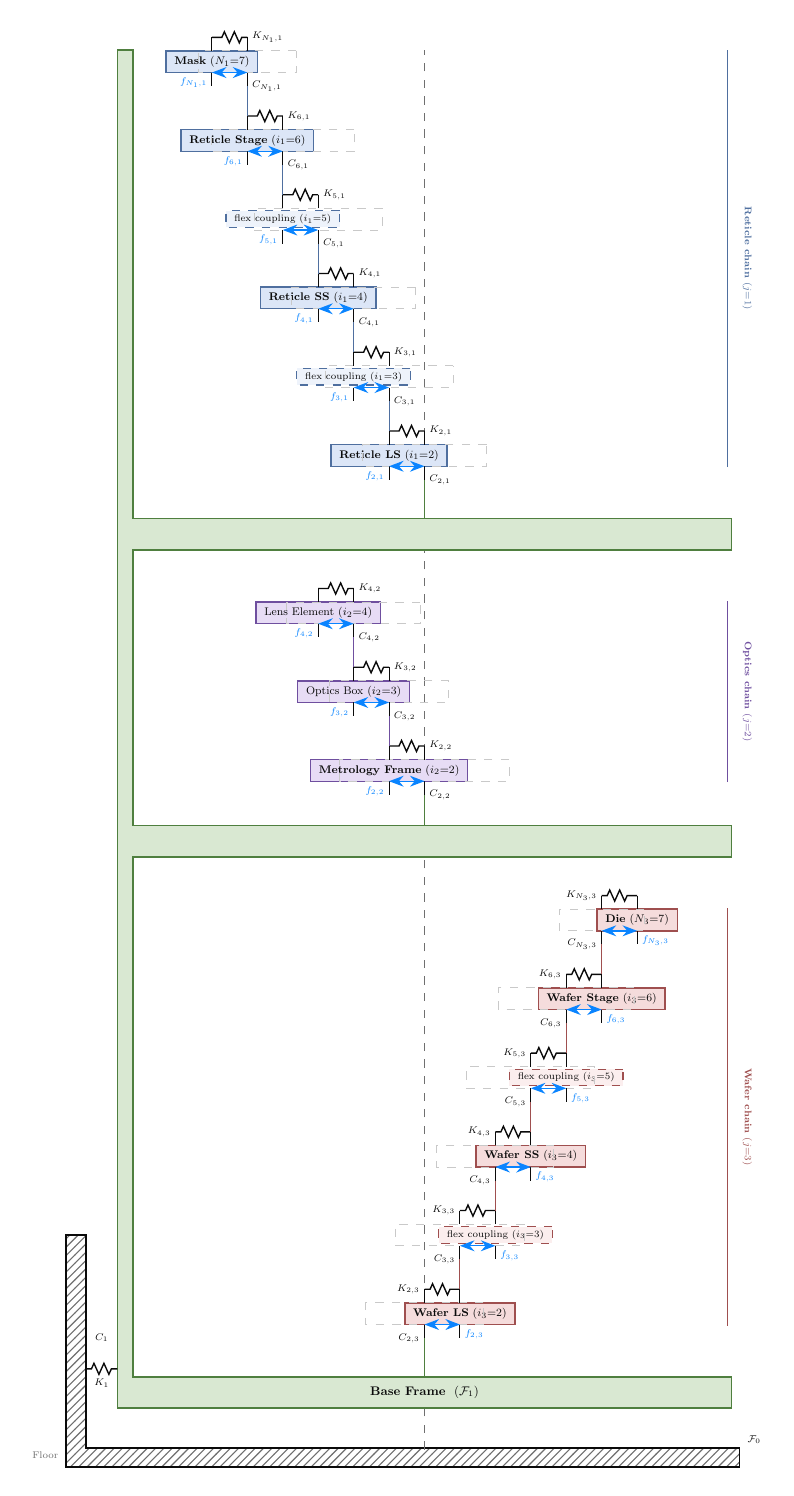
\begin{tikzpicture}[scale=0.5, transform shape,
  every node/.style    ={font=\small},
  rfrm/.style          ={draw=frameEdge, line width=0.6pt, fill=frameFill,
                         minimum height=0.80cm, font=\small\bfseries,
                         inner sep=2pt},
  rblk/.style          ={draw=reticleEdge, line width=0.5pt, fill=reticleFill,
                         minimum height=0.55cm, font=\footnotesize,
                         text=mnnwInk, inner sep=2.5pt},
  rflx/.style          ={draw=reticleEdge, line width=0.4pt, fill=reticleFlex,
                         minimum height=0.42cm, font=\scriptsize,
                         text=mnnwInk, inner sep=2pt, dashed},
  wblk/.style          ={draw=waferEdge, line width=0.5pt, fill=waferFill,
                         minimum height=0.55cm, font=\footnotesize,
                         text=mnnwInk, inner sep=2.5pt},
  wflx/.style          ={draw=waferEdge, line width=0.4pt, fill=waferFlex,
                         minimum height=0.42cm, font=\scriptsize,
                         text=mnnwInk, inner sep=2pt, dashed},
  oblk/.style          ={draw=opticsEdge, line width=0.5pt, fill=opticsFill,
                         minimum height=0.55cm, font=\footnotesize,
                         text=mnnwInk, inner sep=2.5pt},
  oflx/.style          ={draw=opticsEdge, line width=0.4pt, fill=opticsFlex,
                         minimum height=0.42cm, font=\scriptsize,
                         text=mnnwInk, inner sep=2pt, dashed},
  ghost/.style         ={draw=mnnwHair, dashed, line width=0.35pt,
                         fill=none, minimum height=0.55cm},
  hsp/.style           ={line width=0.5pt, mnnwInk, decorate,
                         decoration={zigzag, segment length=3.6pt, amplitude=2pt,
                                     pre length=2pt, post length=2pt}},
  vsp/.style           ={line width=0.5pt, mnnwInk, decorate,
                         decoration={zigzag, segment length=3.6pt, amplitude=2pt,
                                     pre length=2pt, post length=2pt}},
  darr/.style          ={Stealth-Stealth, line width=0.5pt, mnnwSignal},
  lbl/.style           ={font=\scriptsize, text=mnnwInk},
  ftn/.style           ={font=\scriptsize, text=mnnwSignal},
  axis/.style          ={dashed, line width=0.4pt, mnnwMute},
  pillar/.style        ={fill=black!8, draw=mnnwHair, line width=0.3pt},
  hatchfloor/.style    ={pattern=north east lines, pattern color=mnnwMute},
]

% =====================================================================
% Helper macro for one chain body row.
%   #1 y-coord            #2 block-style (rblk/wblk/oblk/rflx/wflx/oflx)
%   #3 previous_x         #4 horizontal offset from Pd (positive = right)
%   #5 block label        #6 K-label   #7 C-label   #8 f-label
% =====================================================================
% Trackers for drawing dashed lines between row couplings
\def\lastSpringY{-100}
\def\lastX{-100}

\def\getfirstchar#1#2\relax{#1}

\newcommand{\chainrow}[8]{%
  % Determine chain color based on style prefix
  \edef\styleName{#2}%
  \def\currColor{mnnwMute}%
  \edef\firstChar{\expandafter\getfirstchar\styleName\relax}%
  \if\firstChar w\def\currColor{waferEdge}\fi
  \if\firstChar o\def\currColor{opticsEdge}\fi
  \if\firstChar r\def\currColor{reticleEdge}\fi

  % Draw dashed line between previous row's spring and current row's damper at the anchor
  \pgfmathparse{abs(#3 - \lastX) < 0.001 ? 1 : 0}
  \ifnum\pgfmathresult=1
    % Use frameEdge if at the centerline (connection to base), else use chain color
    \pgfmathparse{abs(#3) < 0.001 ? 1 : 0}
    \ifnum\pgfmathresult=1
      \def\lineColor{frameEdge}
    \else
      \def\lineColor{\currColor}
    \fi
    \draw[line width=0.35pt, \lineColor] (#3, \lastSpringY) -- (#3, #1-0.62);
  \fi

  % 1. Render the real block first to determine its natural width
  % We use 'inner xsep=6pt' for padding
  \node[#2, inner xsep=6pt] (blk) at (#4,#1) {#5};
  
  % 2. Render the ghost node at the previous x (#3)
  % We use \phantom{#5} so it matches the width/height of the label exactly,
  % but remains completely invisible (empty box)
  \node[ghost, inner xsep=6pt] at (#3,#1) {\phantom{#5}};
  
  % Spring above
  \draw[hsp] (#3, #1+0.62) -- (#4, #1+0.62);
  
  % Anchor lines
  \draw[line width=0.35pt, mnnwInk] (#3, #1+0.275) -- (#3, #1+0.62);
  \draw[line width=0.35pt, mnnwInk] (#4, #1+0.275) -- (#4, #1+0.62);

  % Damper below
  \draw[line width=0.35pt, mnnwInk] (#3, #1-0.275) -- (#3, #1-0.62);
  \draw[line width=0.35pt, mnnwInk] (#4, #1-0.275) -- (#4, #1-0.62);
  
  \hdamperLong{#3}{#4}{#1-0.62}

  % DYNAMIC LABELS (K, C, and f):
  % Logic: If block moves right (#4>#3), place labels on the left (x=#3-0.2, east anchor).
  %        If block moves left (#4<#3), place labels on the right (x=#3+0.2, west anchor).
  \pgfmathsetmacro{\lblSide}{#4 > #3 ? #3 : #3}
  \pgfmathsetmacro{\lblAnch}{#4 > #3 ? "east" : "west"}

  \node[lbl, anchor=\lblAnch] at (\lblSide, #1+0.62) {#6}; % K Label
  \node[lbl, anchor=\lblAnch] at (\lblSide, #1-0.62) {#7}; % C Label
  
  % f label placed at the previous_x axis (#3) but aligned to the same side
  % y-offset of -0.2 matches your deviation arrow's height
  \pgfmathsetmacro{\fSide}{#4 > #3 ? #4 : #4}
  \pgfmathsetmacro{\fAnch}{#4 > #3 ? "west" : "east"}
  \node[ftn, anchor=\fAnch] at (\fSide, #1-0.525) {#8};

  % Deviation arrow (line remains, but label is now at the #3 axis)
  \draw[darr] (#3, #1-0.275) -- (#4, #1-0.275);

  % Update trackers for the next row
  \pgfmathsetmacro{\newSpringY}{#1+0.62}
  \xdef\lastSpringY{\newSpringY}
  \pgfmathsetmacro{\newX}{#4}
  \xdef\lastX{\newX}
}

% =====================================================================
%  GEOMETRY — full stack
% =====================================================================
\def\xLeft{-8.0}\def\xRight{8.0}
\def\xPilL{-7.4}\def\xPilR{7.4}

% Vertical levels (cm). Tight rhythm of 1.6 cm per body row.
% Wafer chain (bodies 2..7 → 6 rows), then F2, then optics (2..4 → 3 rows),
% but per user spec: optics chain attaches around F2 (lens region).
% Layout chosen:
%   F0 floor                  y = 0
%   F1 base frame             y = 1.4
%   Wafer chain  i=2..7       y = 3.2, 4.8, 6.4, 8.0, 9.6, 11.2
%   F2 metrology frame        y = 13.0   (with lens on it)
%   Optics chain  i=2..4      y = 14.4, 15.8, 17.2  (downstream of F2)
%   Reticle chain i=2..7      y = 18.8, 20.4, 22.0, 23.6, 25.2, 26.8
% =====================================================================
\def\yFloor{0}
\def\yBase{1.4}
% Wafer
\def\yWa{3.4}\def\yWb{5.4}\def\yWc{7.4}\def\yWd{9.4}\def\yWe{11.4}\def\yWf{13.4}
% Metrology
% \def\yMet{15.4}
% Optics
\def\yOa{17.2}\def\yOb{19.2}\def\yOc{21.2}
% Reticle
\def\yRa{25.2}\def\yRb{27.2}\def\yRc{29.2}\def\yRd{31.2}\def\yRe{33.2}\def\yRf{35.2}
\def\yTop{35.5}
\def\yShA{15.4}\def\yShB{23.2}

% =====================================================================
%  FLOOR  +  PILLARS  +  Pd
% =====================================================================
\filldraw[hatchfloor, draw=mnnwInk, line width=0.7pt]
  (\xRight, 0) -- (\xLeft-0.6, 0) -- (\xLeft-0.6, \yWb) -- (\xLeft-1.1, \yWb) 
  -- (\xLeft-1.1, -0.5) -- (\xRight, -0.5) -- cycle;
\node[lbl, anchor=west] at (\xRight+0.08,0.20) {$\mathcal{F}_0$};
\node[lbl, anchor=east, text=mnnwMute]
  at (\xLeft-1.1-0.08,-0.18) {Floor};

% \fill[pillar] (\xPilR,0)      rectangle (\xPilR+0.16,\yTop);

\draw[axis] (0,-0.05) -- (0,\yTop);
% \node[font=\small\itshape, anchor=south] at (0,\yTop+0.45) {$P_d$};

% =====================================================================
%  BASE FRAME  F_1
% =====================================================================
\filldraw[draw=frameEdge, line width=0.6pt, fill=frameFill]
  (7.8, \yBase-0.4) -- (-7.8, \yBase-0.4) -- (-7.8, \yTop) -- (-7.4, \yTop)
  -- (-7.4, \yShB+0.4) -- (7.8, \yShB+0.4) -- (7.8, \yShB-0.4) -- (-7.4, \yShB-0.4)
  -- (-7.4, \yShA+0.4) -- (7.8, \yShA+0.4) -- (7.8, \yShA-0.4) -- (-7.4, \yShA-0.4)
  -- (-7.4, \yBase+0.4) -- (7.8, \yBase+0.4) -- cycle;
\node[font=\small\bfseries, text=mnnwInk] at (0, \yBase) {Base Frame $\;(\mathcal{F}_1)$};

% K_1 / C_1  horizontal floor → base frame
\def\lblX{\xLeft-1.2} 

% 1. The Spring (K1)
\hdamperLong{\xLeft-0.6}{-7.8}{2.5}
\node[lbl, above=2pt] at ({(\xLeft-0.6-7.8)/2}, 2.5) {$C_1$};

% 2. The Spring (K1) - Placed on bottom
\draw[hsp] (\xLeft-0.6, 2.0) -- (-7.8, 2.0)
  node[midway, below=4pt, lbl] {$K_1$};

% =====================================================================
%  WAFER CHAIN  (j=3) — light red, blocks shifted RIGHT of Pd
%  i = 2 LS, 3 LS-flex, 4 MS, 5 MS-flex, 6 SS, 7 wafer (N3)
% =====================================================================
\pgfmathsetmacro{\shelfW}{\yBase+0.4}
\xdef\lastSpringY{\shelfW} \xdef\lastX{0}
\chainrow{\yWa}{wblk}{0}{ 0.9}{\textbf{Wafer LS} $(i_3{=}2)$}{$K_{2,3}$}{$C_{2,3}$}{$f_{2,3}$}
\chainrow{\yWb}{wflx}{0.9}{ 1.8}{flex coupling $(i_3{=}3)$}{$K_{3,3}$}{$C_{3,3}$}{$f_{3,3}$}
\chainrow{\yWc}{wblk}{1.8}{ 2.7}{\textbf{Wafer SS} $(i_3{=}4)$}{$K_{4,3}$}{$C_{4,3}$}{$f_{4,3}$}
\chainrow{\yWd}{wflx}{2.7}{ 3.6}{flex coupling $(i_3{=}5)$}{$K_{5,3}$}{$C_{5,3}$}{$f_{5,3}$}
\chainrow{\yWe}{wblk}{3.6}{ 4.5}{\textbf{Wafer Stage} $(i_3{=}6)$}{$K_{6,3}$}{$C_{6,3}$}{$f_{6,3}$}
\chainrow{\yWf}{wblk}{4.5}{ 5.4}{\textbf{Die} $(N_3{=}7)$}{$K_{N_3,3}$}{$C_{N_3,3}$}{$f_{N_3,3}$}

% =====================================================================
%  METROLOGY FRAME  F_2  +  Lens body
% =====================================================================
% \node[rfrm, minimum width=13cm, minimum height=1.0cm] (MF) at (0,\yMet)
%   {Metrology Frame $\;(\mathcal{F}_2)$};
% \node[draw=mnnwInk, line width=0.4pt, fill=lensFill,
%       minimum width=2.4cm, minimum height=0.40cm,
%       font=\scriptsize, anchor=south] at (0,\yMet+0.55) {Lens cell};
% \draw[line width=0.3pt, mnnwInk] (-0.40,\yMet+0.55) -- (-0.75,\yMet+1.05);
% \draw[line width=0.3pt, mnnwInk] ( 0.40,\yMet+0.55) -- ( 0.75,\yMet+1.05);
% \draw[line width=0.3pt, mnnwInk] (-0.40,\yMet-0.10) -- (-0.75,\yMet-0.65);
% \draw[line width=0.3pt, mnnwInk] ( 0.40,\yMet-0.10) -- ( 0.75,\yMet-0.65);

% K_2 / C_2  horizontal pillar → metrology (left side)
% \draw[hsp] (-7.4, \yMet+0.25) -- (-6.5, \yMet+0.25)
%   node[midway, above=2pt, lbl] {$K_{2,2}$};
% \hdamperLong{-7.4}{-6.5}{\yMet-0.25}
% \node[lbl, below] at (-6.95, \yMet-0.38) {$C_{2,2}$};

% =====================================================================
%  OPTICS CHAIN  (j=2)  — light purple, blocks shifted LEFT of Pd
%  Modeled as a 4-body chain whose first body (i=2) attaches to F2.
%  i = 2 lens-frame coarse, i = 3 flex, i = 4 lens cell (N2).
%  Drawn UPWARD from F2 toward the optical axis region.
% =====================================================================
\pgfmathsetmacro{\shelfO}{\yShA+0.4}
\xdef\lastSpringY{\shelfO} \xdef\lastX{0}
\chainrow{\yOa}{oblk}{0}{-0.9}{\textbf{Metrology Frame} $(i_2{=}2)$}{$K_{2,2}$}{$C_{2,2}$}{$f_{2,2}$}
\chainrow{\yOb}{oblk}{-0.9}{-1.8}{Optics Box $(i_2{=}3)$}{$K_{3,2}$}{$C_{3,2}$}{$f_{3,2}$}
\chainrow{\yOc}{oblk}{-1.8}{-2.7}{Lens Element $(i_2{=}4)$}{$K_{4,2}$}{$C_{4,2}$}{$f_{4,2}$}

% =====================================================================
%  RETICLE CHAIN  (j=1) — light blue, blocks shifted LEFT of Pd
%  i = 2 LS, 3 LS-flex, 4 MS, 5 MS-flex, 6 SS, 7 mask (N1)
% =====================================================================
\pgfmathsetmacro{\shelfR}{\yShB+0.4}
\xdef\lastSpringY{\shelfR} \xdef\lastX{0}
\chainrow{\yRa}{rblk}{0}{-0.9}{\textbf{Reticle LS} $(i_1{=}2)$}{$K_{2,1}$}{$C_{2,1}$}{$f_{2,1}$}
\chainrow{\yRb}{rflx}{-0.9}{-1.8}{flex coupling $(i_1{=}3)$}{$K_{3,1}$}{$C_{3,1}$}{$f_{3,1}$}
\chainrow{\yRc}{rblk}{-1.8}{-2.7}{\textbf{Reticle SS} $(i_1{=}4)$}{$K_{4,1}$}{$C_{4,1}$}{$f_{4,1}$}
\chainrow{\yRd}{rflx}{-2.7}{-3.6}{flex coupling $(i_1{=}5)$}{$K_{5,1}$}{$C_{5,1}$}{$f_{5,1}$}
\chainrow{\yRe}{rblk}{-3.6}{-4.5}{\textbf{Reticle Stage} $(i_1{=}6)$}{$K_{6,1}$}{$C_{6,1}$}{$f_{6,1}$}
\chainrow{\yRf}{rblk}{-4.5}{-5.4}{\textbf{Mask} $(N_1{=}7)$}{$K_{N_1,1}$}{$C_{N_1,1}$}{$f_{N_1,1}$}

% =====================================================================
%  CHAIN BRACES  (right edge — quick orienteering)
% =====================================================================
\draw[line width=0.4pt, waferEdge]   (\xPilR+0.30,\yWa-0.30) -- (\xPilR+0.30,\yWf+0.30);
\node[font=\scriptsize\bfseries, text=waferEdge, rotate=-90, anchor=south]
  at (\xPilR+0.55,{(\yWa+\yWf)/2}) {Wafer chain $(j{=}3)$};
\draw[line width=0.4pt, opticsEdge]  (\xPilR+0.30,\yOa-0.30) -- (\xPilR+0.30,\yOc+0.30);
\node[font=\scriptsize\bfseries, text=opticsEdge, rotate=-90, anchor=south]
  at (\xPilR+0.55,{(\yOa+\yOc)/2}) {Optics chain $(j{=}2)$};
\draw[line width=0.4pt, reticleEdge] (\xPilR+0.30,\yRa-0.30) -- (\xPilR+0.30,\yRf+0.30);
\node[font=\scriptsize\bfseries, text=reticleEdge, rotate=-90, anchor=south]
  at (\xPilR+0.55,{(\yRa+\yRf)/2}) {Reticle chain $(j{=}1)$};

\end{tikzpicture}
\caption{Lumped mass-spring-damper system of the three chains vertically stacked on the common base frame}
\label{fig:litho_model_full}
\end{figure}

\section{Dynamics}\label{sec:model_dynamics}

Two distinct joint types arise: \emph{actuated} stages ($i \in \{2,4\}$), which are driven by servo motors and carry a near-infinite effective stiffness that keeps $f_{i_j}$ locked to the nominal reference; and \emph{flex} stages ($i \in \{3,5,6,7\}$), which are passive compliant connections whose stiffness $K_{i_j}$ and damping $C_{i_j}$ are physical material properties of the mechanical coupling.

The full 6-DOF model is here restricted to in-plane motions\cite{Al-Rawashdeh2023_Trajectories,Dong2023_SCurve}, since rotations about the $x$ and $y$ axis, as well as translation on $z$ are used mainly for focusing. The generalized coordinate used to describe the configuration of the $i$th stage within the $j$th chain is
\begin{equation}
    q_{i_j} = \begin{bmatrix} f_{i_j} \\ \theta_{z_{i_j}} \end{bmatrix} \in \mathbb{R}^{3\times1}
\end{equation}
where $f_{i_j} = [f_{x,i_j},\, f_{y,i_j}]^T \in \mathbb{R}^{2}$ collects the in-plane translational displacements of stage $i$ relative to its parent body in chain $j$, and $\theta_{z_{i_j}} \in \mathbb{R}$ is the corresponding rotation about the out-of-plane $z$-axis. The joints between bodies within a chain are modeled using a spring-damper system~\cite{Al-Rawashdeh2022_Caracterization}. The associated generalized mass-inertia matrix for each body is
\begin{equation}
    M_{i_j} = \begin{bmatrix} m_{i_j}\,\mathbf{I}_2 & 0 \\ 0 & I_{z_{i_j}} \end{bmatrix} \in \mathbb{R}^{3\times3}
\end{equation}
and the generalized stiffness and damping matrices $K_{i_j},\, C_{i_j} \in \mathbb{R}^{3\times3}$ are block-diagonal, with a $2\times2$ translational block and a scalar rotational entry.

The absolute position $f^{0}_{i_j}$ of body $i$ is expressed as the recursive sum of its relative displacement from its parent body along the chain from the floor frame $\mathcal{F}_{0}$. Thus, for bodies with $i \geq 2$ on any chain $j \in \{1,2,3\}$:
\begin{equation} \label{eq:frameref}
    f^{0}_{i_j} = f^{0}_{(i-1)_j} + f_{i_j}
\end{equation}

Since the rotation about the $z$-axis is a scalar, the angular position recurrence is simply additive:
\begin{equation} \label{eq:angleref}
    \theta^{0}_{z_{i_j}} = \theta^{0}_{z_{(i-1)_j}} + \theta_{z_{i_j}}
\end{equation}

From this, the translational velocity expression appears as:
\begin{equation}
    \dot{f}^{0}_{i_j} = \dot{f}^{0}_{(i-1)_j} + \dot{f}_{i_j} + \omega_{(i-1)_j}
    \times
    f_{i_j}
\end{equation}

Where $\omega_{(i-1)_j}$ is the angular velocity~\cite{Ginsberg1984_AdvancedDynamics} of $\mathcal{F}_{(i-1)_j}$ with respect to the floor, $\mathcal{F}_{0}$.

Taking the second derivative gives:
\begin{align}
    \begin{split}
        \ddot{f}^{0}_{i_j} &= \ddot{f}^{0}_{(i-1)_j} + \ddot{f}_{i_j}
        + \omega_{(i-1)_j} \times \dot{f}_{i_j}
        + \dot{\omega_{(i-1)_j}} \times f_{i_j}
        + \omega_{(i-1)_j} \times \left[
            \dot{f}_{i_j} + \omega_{(i-1)_j} \times f_{i_j}
        \right] \\
        &= \ddot{f}^{0}_{(i-1)_j} + \ddot{f}_{i_j}
        + \omega_{(i-1)_j} \times \dot{f}_{i_j}
        + \dot{\omega_{(i-1)_j}} \times f_{i_j}
        + \omega_{(i-1)_j} \times \dot{f}_{i_j}
        + \omega_{(i-1)_j} \times \left[
            \omega_{(i-1)_j} \times f_{i_j}
        \right] \\
        &= \ddot{f}^{0}_{(i-1)_j} + \ddot{f}_{i_j}
        + 2 \left[ \omega_{(i-1)_j} \times \dot{f}_{i_j} \right]
        + \dot{\omega_{(i-1)_j}} \times f_{i_j}
        + \omega_{(i-1)_j} \times \left[
            \omega_{(i-1)_j} \times f_{i_j}
        \right]
    \end{split}
\end{align}

Since we are concerned with planar movements in this work, we restrict the angular velocity of each body purely about the $z$-axis as $\omega = \dot{\theta}_z\,\hat{z}$, so that:
\begin{equation}
    \omega_{(i-1)_j} = \dot{\theta}^{0}_{z_{(i-1)_j}}\,\hat{z} \notag
\end{equation}

We substitute the cross-products as matrix-vector products using the skew-symmetric matrix. In the 6-DOF model~\cite{Al-Rawashdeh2022_Caracterization}, it appears as:
\begin{equation}
    [\omega]
    =
    \begin{bmatrix}
        0 & -\omega_z & \omega_y \\
        \omega_z & 0 & -\omega_x \\
        -\omega_y & \omega_x & 0
    \end{bmatrix}
    \notag
\end{equation}
Clearly, here we can set $\omega_x = 0$ and $\omega_y = 0$, thus $\omega = [0,\, 0,\, \dot{\theta}_z]^T$ and the matrix becomes:
\begin{equation}
    [\omega]
    =
    \begin{bmatrix}
        0 & -\omega_z & 0 \\
        \omega_z & 0 & 0 \\
        0 & 0 & 0
    \end{bmatrix}
    \notag
\end{equation}

Considering our 2D displacement vector, we only take the upper-left $2\times2$ 
sub-matrix, and factoring out the scalar $\dot{\theta}^{0}_{z_{(i-1)_j}}$:
\begin{equation} \label{eq:skew}
    [\omega_{(i-1)_j}] = \dot{\theta}^{0}_{z_{(i-1)_j}}
    \begin{bmatrix} 0 & -1 \\ 1 & 0 \end{bmatrix}
\end{equation}
such that $\omega_{(i-1)_j} \times f_{i_j} = [\omega_{(i-1)_j}]\,f_{i_j}$. 
Applying this matrix twice gives the centripetal term:
\begin{equation}
    [\omega_{(i-1)_j}]^2 = -\left(\dot{\theta}^{0}_{z_{(i-1)_j}}\right)^2 \mathbf{I}_2
\end{equation}
so that $\omega_{(i-1)_j} \times [\omega_{(i-1)_j} \times f_{i_j}] =
[\omega_{(i-1)_j}]^2\,f_{i_j}$. Substituting and expanding
\eqref{eq:frameref} recursively from the floor frame, the translational kinematics become:
\begin{align}
    f^{0}_{i_j}
        &= f^{0}_{1} + \sum^{i}_{k=2} f_{k_j}
        \label{eq:pos_expanded} \\
    \dot{f}^{0}_{i_j}
        &= \dot{f}^{0}_{1} + \sum^{i}_{k=2} \dot{f}_{k_j}
         + \sum^{i}_{k=2} [\omega_{(k-1)_j}]\, f_{k_j}
        \label{eq:vel_expanded} \\
    \ddot{f}^{0}_{i_j}
        &= \ddot{f}^{0}_{1} + \sum^{i}_{k=2} \ddot{f}_{k_j}
         + \sum^{i}_{k=2} \left[
             2\,[\omega_{(k-1)_j}]\,\dot{f}_{k_j}
             + [\dot{\omega}_{(k-1)_j}]\,f_{k_j}
             + [\omega_{(k-1)_j}]^2\,f_{k_j}
         \right]
        \label{eq:acc_expanded}
\end{align}

Since the rotation $\theta_{z_{i_j}}$ is a scalar, no Coriolis or centripetal cross-terms arise in the angular kinematics. Expanding~\eqref{eq:angleref} recursively from the floor frame gives the rotational analogues:
\begin{align}
    \theta^{0}_{z_{i_j}}
        &= \theta^{0}_{z_1} + \sum^{i}_{k=2} \theta_{z_{k_j}}
        \label{eq:angle_expanded} \\
    \dot{\theta}^{0}_{z_{i_j}}
        &= \dot{\theta}^{0}_{z_1} + \sum^{i}_{k=2} \dot{\theta}_{z_{k_j}}
        \label{eq:angvel_expanded} \\
    \ddot{\theta}^{0}_{z_{i_j}}
        &= \ddot{\theta}^{0}_{z_1} + \sum^{i}_{k=2} \ddot{\theta}_{z_{k_j}}
        \label{eq:angacc_expanded}
\end{align}

Thus the equation of the angular motion of the $i$th body in the $j$th chain w.r.t $\mathcal{F}_{0}$ is:
\begin{equation}
    {}^{0}\!I_j \, \dot{\omega}_j + \left( [\omega_j] \right) {}^{0}\!I_j \, \omega_j  = m_j^0
\end{equation}

Under the planar restriction $\omega_x = \omega_y = 0$ the gyroscopic term vanishes like:
\begin{equation}
    \left([\omega_{i_j}]\,{}^0\!I_{i_j}\right)\omega_{i_j}
    =
    \begin{bmatrix}
        0 & -\dot{\theta}_z & 0 \\
        \dot{\theta}_z & 0 & 0 \\
        0 & 0 & 0
    \end{bmatrix}
    \begin{bmatrix}
        I_{xx} & 0 & 0 \\
        0 & I_{yy} & 0 \\
        0 & 0 & I_{zz}
    \end{bmatrix}
    \begin{bmatrix}
        0 \\
        0 \\
        \dot{\theta}_z
    \end{bmatrix}
    = 0
    \notag
\end{equation}

Leaving only:
\begin{equation}
    I_{z_{i_j}}\ddot{\theta}^{0}_{z_{i_j}} = m^0_{z_{i_j}}
\end{equation}

where $I_{z_{i_j}}$ is the aggregated moment of inertia of all bodies from $i$ to the end-effector $N_j$, referred to the $z$-axis of body $i$ via Steiner's theorem, and $m^0_{z_{i_j}} \in \mathbb{R}$ is the net applied moment acting on body $i$ in chain $j$ about the $z$-axis.

\paragraph{Steiner's theorem and inertia aggregation.}
The parallel axis (Steiner's) theorem states that the moment of inertia of a rigid body about any axis parallel to one through its center of mass (CoG) satisfies
\begin{equation} \label{eq:steiner}
    I_z = \tilde{I}_z + m\,\|f\|^2,
\end{equation}
where $\tilde{I}_z$ is the body's own moment of inertia about the $z$-axis through its CoG, $m$ is its mass, and $\|f\|^2 = f_x^2 + f_y^2$ is the squared in-plane distance between the two parallel axes. In a serial chain, the inertia of every downstream body must be shifted to the frame of the current body using~\eqref{eq:steiner}. Following the characterization article\cite{Al-Rawashdeh2022_Caracterization} (Algorithm~1 therein), the aggregated inertia for the $j$th chain is computed recursively from the end-effector inward. In the planar restriction, the full $3\times3$ inertia matrix of the original algorithm reduces to a scalar $z$-axis inertia:

\begin{algorithm}[H]
\caption{Planar inertia aggregation for the $j$th chain — planar reduction of Algorithm~1 in~\cite{Al-Rawashdeh2022_Caracterization}}
\begin{algorithmic}[1]
\Require{CoG inertias $\tilde{I}_{z_{i_j}}$, masses $m_{i_j}$, relative positions $f_{k_j}$ for $i = 2,\ldots,N_j$}
\Ensure{Aggregated inertias $^0I_{z_{i_j}}$ for $i = 2,\ldots,N_j$}
\State \textbf{Initialize:} $^0I_{z_{N_j}} \leftarrow \tilde{I}_{z_{N_j}}$
\If{$2 \leq i < N_j$}
    \For{$k = N_j,\;\ldots,\;i+1$}
        \State $\tilde{m}_{(k-1)_j} \leftarrow \displaystyle\sum_{b=k}^{N_j} m_{b_j}$
        \Comment{accumulated downstream mass}
        \State $^0I_{z_{(k-1)_j}} \leftarrow {}^0I_{z_{k_j}} + \tilde{I}_{z_{(k-1)_j}} + \tilde{m}_{(k-1)_j}\bigl(f_{x,k_j}^2 + f_{y,k_j}^2\bigr)$
        \Comment{Steiner shift from frame $k$ to frame $k\!-\!1$}
    \EndFor
\EndIf
\end{algorithmic}
\end{algorithm}

Here $\tilde{m}_{(k-1)_j} = \sum_{b=k}^{N_j} m_{b_j}$ is the total mass of all downstream bodies (from $k$ to the end-effector), $\tilde{I}_{z_{(k-1)_j}}$ is the local inertia of body $k-1$ about its own CoG, and $\tilde{m}_{(k-1)_j}(f_{x,k_j}^2 + f_{y,k_j}^2)$ is the Steiner correction that shifts the accumulated inertia from body $k$'s CoG to body $(k-1)$'s CoG. By the time the algorithm terminates, $^0I_{z_{2_j}}$ contains the inertia of the entire chain $j$ referred to the CoG of its first body.

The aggregated inertia of the base frame (body~1) applies the same shift one more time, from body~2's CoG to the base frame:
\begin{equation} \label{eq:Iz0}
    {}^0I_{z_1} = \tilde{I}_{z_1}
    + \sum_{j=1}^{3}\!\Bigl({}^0I_{z_{2_j}}
      + \tilde{m}_{1_j}\bigl(f_{x,2_j}^2 + f_{y,2_j}^2\bigr)\Bigr),
\end{equation}
where $\tilde{m}_{1_j} = \sum_{b=2}^{N_j} m_{b_j}$ is the total mass of chain $j$. This is the quantity denoted $I_{z_0}$ in~\eqref{eq:baseframerot}.

Expanding $\ddot{\theta}^0_{z_{i_j}}$ using~\eqref{eq:angacc_expanded}:
\begin{equation} \label{eq:torqueeq_expanded}
    I_{z_{i_j}}\ddot{\theta}^{0}_{z_1} 
    + I_{z_{i_j}}\sum^{i}_{k=2}\ddot{\theta}_{z_{k_j}}
    = m^0_{z_{i_j}}
\end{equation}

\subsection{For the base frame}

To write the equations that govern the base frame, we start from Newton's equation $F = ma$. For every body ($i \geq 2$) within chain $j$, it connects to body $i-1$ through a spring above and body $i+1$ through the spring below:
\begin{align} \label{eq:forceeq}
    \begin{split}
        m_{i_j}\ddot{f}^{0}_{1}
        + m_{i_j}\sum^{i}_{k=2}\ddot{f}_{k_j}
        + m_{i_j}\sum^{i}_{k=2}
        &\left[
            2\,[\omega_{(k-1)_j}]\,\dot{f}_{k_j}
            + [\dot{\omega}_{(k-1)_j}]\,f_{k_j}
            + [\omega_{(k-1)_j}]^2\,f_{k_j}
        \right] \\
        - K_i\left( f^0_{{(i-1)}_j} - f^0_{{i}_j}\right)
        - C_i\left( \dot{f}^0_{{(i-1)}_j} - \dot{f}^0_{{i}_j}\right)
        &+ K_{i+1}\left( f^0_{{i}_j} - f^0_{{(i+1)}_j}\right)
        + C_{i+1}\left( \dot{f}^0_{{i}_j} - \dot{f}^0_{{(i+1)}_j}\right)
        = u^0_{i_j}
    \end{split}
\end{align}

Summing~\eqref{eq:forceeq} over all bodies in a chain (taking the optics chain $j=2$, bodies $i=2,3,4$ as a representative example), the internal spring forces cancel by Newton's third law:
\begin{align}
    &- K_2(f^0_1 - f^0_2) - C_2(\dot{f}^0_1 - \dot{f}^0_2) \notag \\
    &\quad \cancelto{0}{
        + K_3(f^0_2 - f^0_3) + C_3(\dot{f}^0_2 - \dot{f}^0_3)
        - K_3(f^0_2 - f^0_3) - C_3(\dot{f}^0_2 - \dot{f}^0_3)
    } \notag \\
    &\quad \cancelto{0}{
        + K_4(f^0_3 - f^0_4) + C_4(\dot{f}^0_3 - \dot{f}^0_4)
        - K_4(f^0_3 - f^0_4) - C_4(\dot{f}^0_3 - \dot{f}^0_4)
    } \notag
\end{align}

Only the boundary term $- K_2(f^0_1 - f^0_2) - C_2(\dot{f}^0_1 - \dot{f}^0_2)$ survives, which corresponds to the connection between body $i = 2$ and the base frame. This extends to any $N_j$-body chain. Recalling~\eqref{eq:frameref}, $f^{0}_{1} - f^{0}_{2_j} = -f_{2_j}$, and following~\cite{Al-Rawashdeh2022_Caracterization} with ${}^0K_{i_j}={}^0R_{i_j} K_{i_j} {}^0R^T_{i_j}$ and ${}^0C_{i_j}={}^0R_{i_j} C_{i_j} {}^0R^T_{i_j}$, the total translational equation of the base frame (absorbing the balance masses and collecting all chain contributions) is:
\begin{align} \label{eq:baseframeeq}
    \begin{split}
        m_0\,\ddot{f}^{0}_{1}
        + {}^0\bar{C}_1\,\dot{f}_1
        + {}^0\bar{K}_1\,f_1
        - \sum_{j=1}^{3}\left\{
            {}^0\hat{C}_{2_j}\,\dot{f}_{2_j} + {}^0\hat{K}_{2_j}\,f_{2_j}
        \right\}
        &= u^0_{1}
    \end{split}
\end{align}
where $m_0 = m_{1} + \sum_{j=1}^{3}\!\left(m^j_{B} + \sum_{i=2}^{N_j} m_{i_j}\right)$ is the total system mass, and the stiffness and damping matrices denote the $2\times2$ translational block. Following~\cite{Al-Rawashdeh2022_Caracterization}, ${}^0\bar{K}_1 = {}^0K_1$ and ${}^0\bar{C}_1 = {}^0C_1$, while the hatted chain couplings are ${}^0\hat{C}_{2_j} = {}^0C_{2_j}$ and ${}^0\hat{K}_{2_j} = {}^0K_{2_j} + {}^0C_{2_j}[\omega_1]$; the accents are defined in general in~\eqref{eq:accented} below.

By the exact same cancellation argument applied to the moment balance about the $z$-axis — the moment exerted by the spring connecting body $i$ to body $i-1$ is $-K_{i_j}\,\theta_{z_{i_j}}$, so internal moments cancel identically — the rotational equation of the base frame is:
\begin{align} \label{eq:baseframerot}
    \begin{split}
        I_{z_0}\,\ddot{\theta}^{0}_{z_1}
        + {}^0\bar{C}_1\,\dot{\theta}_{z_1}
        + {}^0\bar{K}_1\,\theta_{z_1}
        - \sum_{j=1}^{3}\left\{
            {}^0\hat{C}_{2_j}\,\dot{\theta}_{z_{2_j}}
            + {}^0\hat{K}_{2_j}\,\theta_{z_{2_j}}
        \right\}
        &= \tau^0_{1}
    \end{split}
\end{align}
where $I_{z_0} = I_{z_1} + \sum_{j=1}^{3}\!\left(I^j_{z_B} + \sum_{i=2}^{N_j} I_{z_{i_j}}\right)$ is the total moment of inertia of the system about the $z$-axis, ${}^0\bar{C}_{i_j}$ and ${}^0\bar{K}_{i_j}$ (and their hatted counterparts, which coincide with them for the scalar rotational entries) are the scalar rotational damping and stiffness of the joint connecting body $i$ to its predecessor in chain $j$, and $\tau^0_1$ is the net applied torque on the base frame.

\subsection{For each chain}

Recalling~\eqref{eq:forceeq} and~\eqref{eq:torqueeq_expanded}, for the first body in the chain ($i=2$), which connects to the base frame above and to body $i=3$ below, the translational equation is:
\begin{equation}
        \bar{m}_{2_j}
        \ddot{f}^{0}_{2_j}
        + {}^0\bar{C}_{2_j}\,\dot{f}_{2_j}
        + {}^0\bar{K}_{2_j}\,f_{2_j}
        - \left\{
            {}^0\hat{C}_{3_j}\,\dot{f}_{3_j} + {}^0\hat{K}_{3_j}\,f_{3_j}
        \right\}
        = u^0_{2_j}
\end{equation}
and the rotational equation is:
\begin{equation}
        I_{z_{2_j}}\ddot{\theta}^{0}_{z_{2_j}}
        + {}^0\bar{C}_{2_j}\,\dot{\theta}_{z_{2_j}}
        + {}^0\bar{K}_{2_j}\,\theta_{z_{2_j}}
        - {}^0\hat{C}_{3_j}\,\dot{\theta}_{z_{3_j}}
        - {}^0\hat{K}_{3_j}\,\theta_{z_{3_j}}
        = \tau^0_{2_j}
\end{equation}

For bodies $3\leq i< N_j$, the same structure holds with bodies $2, \dots, i-1$ in between. The translational equation is:
\begin{equation}
        \bar{m}_{i_j}
        \ddot{f}^{0}_{i_j}
        + {}^0\bar{C}_{i_j}\,\dot{f}_{i_j}
        + {}^0\bar{K}_{i_j}\,f_{i_j}
        -
        \left\{
            {}^0\hat{C}_{(i+1)_j}\,\dot{f}_{(i+1)_j} + {}^0\hat{K}_{(i+1)_j}\,f_{(i+1)_j}
        \right\}
        = u^0_{i_j}
\end{equation}
and the rotational equation is:
\begin{equation}
        I_{z_{i_j}}\ddot{\theta}^{0}_{z_{i_j}}
        + {}^0\bar{C}_{i_j}\,\dot{\theta}_{z_{i_j}}
        + {}^0\bar{K}_{i_j}\,\theta_{z_{i_j}}
        - {}^0\hat{C}_{(i+1)_j}\,\dot{\theta}_{z_{(i+1)_j}}
        - {}^0\hat{K}_{(i+1)_j}\,\theta_{z_{(i+1)_j}}
        = \tau^0_{i_j}
\end{equation}

Finally, for body $i = N_j$ (the end effector), there is no subsequent body in the chain. The translational and rotational equations are:
\begin{equation}
        \bar{m}_{{N_j}_j}
        \ddot{f}^{0}_{{N_j}_j}
        + {}^0\bar{C}_{{N_j}_j}\,\dot{f}_{{N_j}_j}
        + {}^0\bar{K}_{{N_j}_j}\,f_{{N_j}_j}
        = 0
\end{equation}
\begin{equation}
        I_{z_{{N_j}_j}}\ddot{\theta}^{0}_{z_{{N_j}_j}}
        + {}^0\bar{C}_{{N_j}_j}\,\dot{\theta}_{z_{{N_j}_j}}
        + {}^0\bar{K}_{{N_j}_j}\,\theta_{z_{{N_j}_j}}
        = 0
\end{equation}

\subsection{Accented matrices and the nominal condition}

Following Appendix~A of~\cite{Al-Rawashdeh2022_Caracterization}, the accented matrices appearing in the equations above are not merely rotated joint matrices: they absorb the rotational cross-terms of~\eqref{eq:acc_expanded} into effective damping and stiffness. With $[\omega]$ the planar skew form of~\eqref{eq:skew} and $B_{i_j} = [\dot{\omega}_{i_j}] + [\omega_{i_j}]^2$:
\begin{align}
    \bar{m}_{i_j} &= \sum_{k=i}^{N_j} m_{k_j} \notag \\
    {}^0\bar{C}_{i_j} &= {}^0C_{i_j} + 2m_{i_j}\,[\omega_{(i-1)_j}] \notag \\
    {}^0\bar{K}_{i_j} &= {}^0K_{i_j} + {}^0C_{i_j}\,[\omega_{(i-1)_j}] + m_{i_j}\,B_{(i-1)_j} \label{eq:accented} \\
    {}^0\hat{C}_{(i+1)_j} &= {}^0C_{(i+1)_j} \notag \\
    {}^0\hat{K}_{(i+1)_j} &= {}^0K_{(i+1)_j} + {}^0C_{(i+1)_j}\,[\omega_{i_j}] \notag
\end{align}
The bar thus marks the matrices acting on the body's \emph{own} joint coordinates, which collect the Coriolis ($2m[\omega]$), damper-convection ($C[\omega]$), and Euler--centripetal ($mB$) contributions, while the hat marks the coupling to the \emph{downstream} joint coordinates, which inherits only the convective damper term: the damper reacts to the inertial velocity $\dot{f} + [\omega]f$ of~\eqref{eq:vel_expanded}, so part of its force is proportional to position and migrates into the effective stiffness. The scalar rotational entries admit no such cross-terms in the planar restriction, so about the $z$-axis the accents are inert and $\hat{(\cdot)} = \bar{(\cdot)} = (\cdot)$. For $3 \leq i < N_j$ the model of~\cite{Al-Rawashdeh2022_Caracterization} additionally couples body $i$ to every upstream joint through the two-index matrices ${}^0\hat{C}_{i_j,k} = 2m_{i_j}\,[\omega_{(k-1)_j}]$ and ${}^0\hat{K}_{i_j,k} = m_{i_j}\,B_{(k-1)_j}$ for $2 \leq k < i$, omitted above.

Every one of these corrections is proportional to $\dot{\theta}_z$ or $\ddot{\theta}_z$ of a parent body. At the nominal operating condition $\dot{\theta}_z = \ddot{\theta}_z = 0$ --- the regulated step-and-scan regime studied throughout this work --- they vanish identically: the accented matrices reduce to the frame-rotated ${}^0K_{i_j}$ and ${}^0C_{i_j}$, the inertial accelerations of~\eqref{eq:acc_expanded} reduce to sums of relative accelerations, and the equations of motion coincide with Eqs.~(2.6)--(2.8) of~\cite{Al-Rawashdeh2022_Caracterization} and become linear time-invariant. Away from the nominal condition, the corrections re-enter as the parameter-varying part $A_1(\Omega,\dot{\Omega})$ of the decomposition given in~\cite{Al-Rawashdeh2022_Caracterization}. Note that the scheduling variables $\Omega$ are themselves state variables --- the $\dot{\theta}_z$ of each body --- so the cross-terms are quadratic in the state (and the rotated matrices ${}^0K_{i_j}$, ${}^0C_{i_j}$ carry a further state dependence through ${}^0R_{i_j}(\theta_z)$): the machine model is, strictly, nonlinear, a \emph{quasi}-LPV system whose frozen nominal dynamics are the LTI model above. The MuJoCo test bed used throughout this work assembles the full nonlinear multibody dynamics from this lumped topology directly, retaining these couplings without approximation; the LTI form above is recovered only as its frozen nominal dynamics at $\dot{\theta}_z = \ddot{\theta}_z = 0$, not as a separately integrated reduced model.

\subsection{State-space formulation}

Because each body possesses three planar degrees of freedom ($f_x$, $f_y$, $\theta_z$) along with their corresponding time derivatives, it contributes exactly six states to the system. Following the machine description of~\cite{Al-Rawashdeh2022_Caracterization} (Section~2.2 therein), the complete machine model comprises 6 bodies in the reticle chain ($N_1 = 7$), 3 bodies in the optics chain ($N_2 = 4$), and 6 bodies in the wafer chain ($N_3 = 7$). Including the common base frame (body 1), the system features a total of $1 + (N_1-1) + (N_2-1) + (N_3-1) = 16$ bodies. Consequently, the global state vector $x$ encompasses $6 \times 16 = 96$ states:

\begin{equation}
    x =
    \begin{bmatrix}
        \underbrace{x_1, \ldots, x_6}_{\text{base frame}} \;,\;
        \underbrace{x_7, \ldots, x_{6N_1}}_{\text{chain 1: bodies } 2 \to N_1} \;,\;
        \underbrace{\ldots}_{\text{chain 2}} \;,\;
        \underbrace{\ldots}_{\text{chain 3}}
    \end{bmatrix}^T
\end{equation}

The explicit mapping for each state is detailed in the table below. Here, $p$ denotes the global sequential index of the $i$-th body in the $j$-th chain within the concatenated list of all bodies (starting with the base frame, followed sequentially by chains 1, 2, and 3). It is crucial to note that every positional entry within the state vector represents a \emph{relative} joint displacement; the corresponding absolute inertial position $f^0_{i_j}$ can be reconstructed using the recursive summations from~\eqref{eq:pos_expanded} to~\eqref{eq:angle_expanded}.

\begin{table}[htbp]
\centering
\caption{State-space mapping for the global concatenated system vector}
\label{tab:state_mapping}
\begin{tabular}{cll}
\toprule
State-space Variable & Expression & Meaning \\
\midrule
$x_1$       & $f_{x_1}$                  & base frame $x$-position \\
$x_2$       & $f_{y_1}$                  & base frame $y$-position \\
$x_3$       & $\theta_{z_1}$             & base frame rotation \\
$x_4$       & $\dot{f}_{x_1}$            & base frame $x$-velocity \\
$x_5$       & $\dot{f}_{y_1}$            & base frame $y$-velocity \\
$x_6$       & $\dot{\theta}_{z_1}$       & base frame angular velocity \\
$x_7$       & $f_{x_{2_1}}$              & chain 1, body 2, $x$-position \\
$x_8$       & $f_{y_{2_1}}$              & chain 1, body 2, $y$-position \\
$x_9$       & $\theta_{z_{2_1}}$         & chain 1, body 2, rotation \\
$x_{10}$    & $\dot{f}_{x_{2_1}}$        & chain 1, body 2, $x$-velocity \\
$x_{11}$    & $\dot{f}_{y_{2_1}}$        & chain 1, body 2, $y$-velocity \\
$x_{12}$    & $\dot{\theta}_{z_{2_1}}$   & chain 1, body 2, angular velocity \\
$\vdots$    & $\vdots$                   & $\vdots$ \\
$x_{6p-5}$  & $f_{x_{i_j}}$              & chain $j$, body $i$, $x$-position \\
$x_{6p-4}$  & $f_{y_{i_j}}$              & chain $j$, body $i$, $y$-position \\
$x_{6p-3}$  & $\theta_{z_{i_j}}$         & chain $j$, body $i$, rotation \\
$x_{6p-2}$  & $\dot{f}_{x_{i_j}}$        & chain $j$, body $i$, $x$-velocity \\
$x_{6p-1}$  & $\dot{f}_{y_{i_j}}$        & chain $j$, body $i$, $y$-velocity \\
$x_{6p}$    & $\dot{\theta}_{z_{i_j}}$   & chain $j$, body $i$, angular velocity \\
$\vdots$    & $\vdots$                   & $\vdots$ \\
\bottomrule
\end{tabular}
\end{table}

Solving~\eqref{eq:baseframeeq} and~\eqref{eq:baseframerot} for the base-frame accelerations yields:
\begin{align}
    \ddot{f}^{0}_{1}
    &= -\frac{{}^0\bar{C}_1}{m_0}\,\dot{f}_1
       -\frac{{}^0\bar{K}_1}{m_0}\,f_1
       +\frac{1}{m_0}\sum_{j=1}^{3}\left\{
           {}^0\bar{C}_{2_j}\,\dot{f}_{2_j} + {}^0\bar{K}_{2_j}\,f_{2_j}
       \right\}
       +\frac{u^0_{1}}{m_0} \label{eq:f1ddot} \\[4pt]
    \ddot{\theta}^{0}_{z_1}
    &= -\frac{{}^0\bar{C}_1}{I_{z_0}}\,\dot{\theta}_{z_1}
       -\frac{{}^0\bar{K}_1}{I_{z_0}}\,\theta_{z_1}
       +\frac{1}{I_{z_0}}\sum_{j=1}^{3}\left\{
           {}^0\bar{C}_{2_j}\,\dot{\theta}_{z_{2_j}} + {}^0\bar{K}_{2_j}\,\theta_{z_{2_j}}
       \right\}
       +\frac{\tau^0_{1}}{I_{z_0}} \label{eq:th1ddot}
\end{align}

Expressed in the standard matrix form $\dot{x} = Ax + Bu$, the first six rows governing the base-frame dynamics are:
\setcounter{MaxMatrixCols}{20}
\begin{equation}
\begin{bmatrix}\dot{x}_1\\\dot{x}_2\\\dot{x}_3\\\dot{x}_4\\\dot{x}_5\\\dot{x}_6\end{bmatrix}
=
\begin{bmatrix}
    0 & 0 & 0 & 1 & 0 & 0 & 0 & 0 & 0 & 0 & \cdots \\
    0 & 0 & 0 & 0 & 1 & 0 & 0 & 0 & 0 & 0 & \cdots \\
    0 & 0 & 0 & 0 & 0 & 1 & 0 & 0 & 0 & 0 & \cdots \\
    -\frac{K_{1,xx}}{m_0} & -\frac{K_{1,xy}}{m_0} & 0 &
    -\frac{C_{1,xx}}{m_0} & -\frac{C_{1,xy}}{m_0} & 0 &
    \frac{K_{2_1,xx}}{m_0} & \frac{K_{2_1,xy}}{m_0} & 0 &
    \frac{C_{2_1,xx}}{m_0} & \cdots \\
    -\frac{K_{1,yx}}{m_0} & -\frac{K_{1,yy}}{m_0} & 0 &
    -\frac{C_{1,yx}}{m_0} & -\frac{C_{1,yy}}{m_0} & 0 &
    \frac{K_{2_1,yx}}{m_0} & \frac{K_{2_1,yy}}{m_0} & 0 &
    \frac{C_{2_1,yx}}{m_0} & \cdots \\
    0 & 0 & -\frac{K_{1,zz}}{I_{z_0}} & 0 & 0 &
    -\frac{C_{1,zz}}{I_{z_0}} & 0 & 0 &
    \frac{K_{2_1,zz}}{I_{z_0}} & 0 & \cdots \\
\end{bmatrix}
x
+
\begin{bmatrix}
    0 & 0 & 0 & \cdots \\
    0 & 0 & 0 & \cdots \\
    0 & 0 & 0 & \cdots \\
    \frac{1}{m_0} & 0 & 0 & \cdots \\
    0 & \frac{1}{m_0} & 0 & \cdots \\
    0 & 0 & \frac{1}{I_{z_0}} & \cdots
\end{bmatrix}
\begin{bmatrix}u^0_{x,1}\\u^0_{y,1}\\\tau^0_1\\\vdots\end{bmatrix}
\end{equation}

\subsubsection{General State-Space Form for the Chain Bodies}

To systematically construct the global state-space matrices, we must reframe the equations of motion for the chain bodies in terms of the state vector variables. We map the physical planar coordinates of the $p$-th sequential body to the local state vectors: translational position $\mathbf{x}_{2p-1} = [x_{6p-5},\, x_{6p-4}]^T$, translational velocity $\dot{\mathbf{x}}_{2p-1} = [x_{6p-2},\, x_{6p-1}]^T$, rotational position $\mathbf{x}_{2p} = x_{6p-3}$, and rotational velocity $\dot{\mathbf{x}}_{2p} = x_{6p}$.

The state derivatives are dictated by the relative accelerations between adjacent bodies. By applying the kinematic identity $\ddot{f}_{i_j} = \ddot{f}^0_{i_j} - \ddot{f}^0_{(i-1)_j}$ from~\eqref{eq:acc_expanded}, we determine the interactive forces acting on each body within its parent's reference frame. Let $p$ represent the global index of body $i$ in chain $j$, while $p-1$ and $p+1$ denote the indices of its immediate upstream and downstream neighbors respectively (with the base frame positioned at $p=1$). 


For the \textbf{first body in each chain} ($i=2$, index $p$, upstream index $1$), the translational state derivatives ($\ddot{\mathbf{x}}_{2p-1} = \ddot{f}_{2_j}$) and rotational state derivatives ($\ddot{\mathbf{x}}_{2p} = \ddot{\theta}_{z_{2_j}}$) take the form:
\begin{align}
    \ddot{\mathbf{x}}_{2p-1} &= 
    \frac{1}{\bar{m}_{2_j}} \Big[ u^0_{2_j} - {}^0\bar{C}_{2_j}\dot{\mathbf{x}}_{2p-1} - {}^0\bar{K}_{2_j}\mathbf{x}_{2p-1} + {}^0\hat{C}_{3_j}\dot{\mathbf{x}}_{2p+1} + {}^0\hat{K}_{3_j}\mathbf{x}_{2p+1} \Big] \notag \\
    &\quad - \frac{1}{m_0} \Big[ u^0_1 - {}^0\bar{C}_1\dot{\mathbf{x}}_{1} - {}^0\bar{K}_1 \mathbf{x}_{1} + \sum_{k=1}^3 \left( {}^0\hat{C}_{2_k}\dot{\mathbf{x}}_{2p_{2_k}-1} + {}^0\hat{K}_{2_k}\mathbf{x}_{2p_{2_k}-1} \right) \Big] \\
    \ddot{\mathbf{x}}_{2p} &= 
    \frac{1}{I_{z_{2_j}}} \Big[ \tau^0_{2_j} - {}^0\bar{c}_{\theta,2_j}\dot{\mathbf{x}}_{2p} - {}^0\bar{k}_{\theta,2_j}\mathbf{x}_{2p} + {}^0\hat{c}_{\theta,3_j}\dot{\mathbf{x}}_{2p+2} + {}^0\hat{k}_{\theta,3_j}\mathbf{x}_{2p+2} \Big] \notag \\
    &\quad - \frac{1}{I_{z_0}} \Big[ \tau^0_1 - {}^0\bar{C}_1\dot{\mathbf{x}}_{2} - {}^0\bar{K}_1 \mathbf{x}_{2} + \sum_{k=1}^3 \left( {}^0\hat{c}_{\theta,2_k}\dot{\mathbf{x}}_{2p_{2_k}} + {}^0\hat{k}_{\theta,2_k}\mathbf{x}_{2p_{2_k}} \right) \Big]
\end{align}

For a \textbf{general intermediate body} ($2 < i < N_j$, index $p$), the dynamics are shaped by upstream, local, and downstream interactions:
\begin{align}
    \ddot{\mathbf{x}}_{2p-1} &= 
    \frac{1}{\bar{m}_{i_j}} \Big[ u^0_{i_j} - {}^0\bar{C}_{i_j}\dot{\mathbf{x}}_{2p-1} - {}^0\bar{K}_{i_j}\mathbf{x}_{2p-1} + {}^0\hat{C}_{(i+1)_j}\dot{\mathbf{x}}_{2p+1} + {}^0\hat{K}_{(i+1)_j}\mathbf{x}_{2p+1} \Big] \notag \\
    &\quad - \frac{1}{\bar{m}_{(i-1)_j}} \Big[ u^0_{(i-1)_j} - {}^0\bar{C}_{(i-1)_j}\dot{\mathbf{x}}_{2p-3} - {}^0\bar{K}_{(i-1)_j}\mathbf{x}_{2p-3} + {}^0\hat{C}_{i_j}\dot{\mathbf{x}}_{2p-1} + {}^0\hat{K}_{i_j}\mathbf{x}_{2p-1} \Big] \\
    \ddot{\mathbf{x}}_{2p} &= 
    \frac{1}{I_{z_{i_j}}} \Big[ \tau^0_{i_j} - {}^0\bar{c}_{\theta,i_j}\dot{\mathbf{x}}_{2p} - {}^0\bar{k}_{\theta,i_j}\mathbf{x}_{2p} + {}^0\hat{c}_{\theta,(i+1)_j}\dot{\mathbf{x}}_{2p+2} + {}^0\hat{k}_{\theta,(i+1)_j}\mathbf{x}_{2p+2} \Big] \notag \\
    &\quad - \frac{1}{I_{z_{(i-1)_j}}} \Big[ \tau^0_{(i-1)_j} - {}^0\bar{c}_{\theta,(i-1)_j}\dot{\mathbf{x}}_{2p-2} - {}^0\bar{k}_{\theta,(i-1)_j}\mathbf{x}_{2p-2} + {}^0\hat{c}_{\theta,i_j}\dot{\mathbf{x}}_{2p} + {}^0\hat{k}_{\theta,i_j}\mathbf{x}_{2p} \Big]
\end{align}

Finally, for the \textbf{end-effector body} ($i = N_j$, index $p$), the downstream force terms naturally vanish as there are no subsequent bodies:
\begin{align}
    \ddot{\mathbf{x}}_{2p-1} &= 
    \frac{1}{\bar{m}_{{N_j}_j}} \Big[ u^0_{{N_j}_j} - {}^0\bar{C}_{{N_j}_j}\dot{\mathbf{x}}_{2p-1} - {}^0\bar{K}_{{N_j}_j}\mathbf{x}_{2p-1} \Big] \notag \\
    &\quad - \frac{1}{\bar{m}_{({N_j}-1)_j}} \Big[ u^0_{({N_j}-1)_j} - {}^0\bar{C}_{({N_j}-1)_j}\dot{\mathbf{x}}_{2p-3} - {}^0\bar{K}_{({N_j}-1)_j}\mathbf{x}_{2p-3} + {}^0\hat{C}_{{N_j}_j}\dot{\mathbf{x}}_{2p-1} + {}^0\hat{K}_{{N_j}_j}\mathbf{x}_{2p-1} \Big] \\
    \ddot{\mathbf{x}}_{2p} &= 
    \frac{1}{I_{z_{{N_j}_j}}} \Big[ \tau^0_{{N_j}_j} - {}^0\bar{c}_{\theta,{N_j}_j}\dot{\mathbf{x}}_{2p} - {}^0\bar{k}_{\theta,{N_j}_j}\mathbf{x}_{2p} \Big] \notag \\
    &\quad - \frac{1}{I_{z_{({N_j}-1)_j}}} \Big[ \tau^0_{({N_j}-1)_j} - {}^0\bar{c}_{\theta,({N_j}-1)_j}\dot{\mathbf{x}}_{2p-2} - {}^0\bar{k}_{\theta,({N_j}-1)_j}\mathbf{x}_{2p-2} + {}^0\hat{c}_{\theta,{N_j}_j}\dot{\mathbf{x}}_{2p} + {}^0\hat{k}_{\theta,{N_j}_j}\mathbf{x}_{2p} \Big]
\end{align}

\def\baselinestretch{1}

\chapter{Control Objectives}\label{ch:control_objectives}

\def\baselinestretch{1.66}

\section{Introduction}\label{sec:control_introduction}

In Chapter~\ref{ch:introduction} we identified overlay and throughput as the two primary drivers of scanner design, followed in Chapter~\ref{ch:model} by the modeling of its multi-body dynamics. This chapter focuses on mapping those industrial requirements into quantitative objectives that any candidate reference trajectory must satisfy. Here we explore in detail how the synchronization error arises between the wafer and the reticle stages, examine the filtered metrics through which the industry evaluates it, and establish the formal statement of the optimization problem.

\section{Synchronization Error}\label{sec:control_synchronization}

During the scanning exposure, the projection optics image the reticle onto the wafer with a demagnification factor of $\alpha = 0.25$. Thus, the image of the reticle pattern is stationary on the wafer surface only if the wafer follows the reticle motion scaled by $\alpha$ at every instant. The degradation of the printed pattern is therefore not due to the individual tracking error of either stage, but their scaled difference. Let $r_w(t)$ and $r_r(t)$ denote the reference positions of the wafer and reticle stages respectively along the scanning direction, and $y_w(t)$, $y_r(t)$ their measured positions. The \textit{synchronization error} is defined as~\cite{Butler2011_PositionControl}
\begin{equation}
    e_{syn}(t) = \big(y_w(t) - r_w(t)\big) - \alpha \big(y_r(t) - r_r(t)\big).
    \label{eq:esyn}
\end{equation}
Naturally, a common-mode mode disturbance that displaces both stages consistently with the projection ratio leaves $e_{syn}$ unaffected. Conversely, any differential motion between the chains --- exacerbated by the lightly damped structural resonance --- is transferred directly to the printed image.

\section{Exposure Metrics: MA and MSD}\label{sec:control_ma_msd}

For an area of photoresist to become exposed, the illumination dose must overcome a threshold. Despite direct exposure during the scanning motion, the photoresist on the wafer does not respond to the instantaneous value of $e_{syn}$ but to its aggregate effect over the time a given point stays below the light source. Therefore, industry practice evaluates the synchronization error through two moving-window filters matched to the exposure time $t_{exp}$ of one point on the wafer~\cite{Butler2011_PositionControl}:

\begin{itemize}
    \item First, the \textbf{moving average}
    \begin{equation}
        \mathrm{MA}(t_k) = \frac{1}{N}\sum_{n=0}^{N-1} e_{syn}(t_{k-n})
        \label{eq:ma}
    \end{equation}
    measures the mean displacement of the image and manifests as \textit{overlay} error or the misalignment of the printed pattern with respect to the previous layer.

    \item Second, the \textbf{moving standard deviation}
    \begin{equation}
        \mathrm{MSD}(t_k) = \sqrt{\frac{1}{N}\sum_{n=0}^{N-1} \Big(e_{syn}(t_{k-n}) - \mathrm{MA}(t_k)\Big)^{2}}
        \label{eq:msd}
    \end{equation}
    measures the smearing of the aerial image around that mean position and manifests as \textit{fading}, a loss of contrast that distorts the printed feature.
\end{itemize}

For the 38\,nm half-pitch process, the specifications adopted~\cite{Al-Rawashdeh2022_Caracterization} are
\begin{equation}
    \mathrm{MA} \in [-1.25,\ +2]\ \mathrm{nm}, \qquad \mathrm{MSD} \leq 7\ \mathrm{nm},
    \label{eq:ma_msd_spec}
\end{equation}
evaluated at every instant during the exposure window~\cite{Butler2011_PositionControl}. These bounds must be met while the stage sustains the required scanning velocity, operating within a settling time budget of under $10\,\mathrm{ms}$ to preserve wafer throughput. On the two-stage machine modelled here they are not a fixed pass/fail but the tight end of a trade curve: Chapter~\ref{ch:experiments} shows that a sufficiently smooth fourth-order trajectory meets them --- both MSD and MA, to the nanometer --- at the cost of a longer scan, so the specification and the throughput budget are the two ends of the optimization this thesis performs.

\section{Problem Statement}\label{sec:control_problem}

The reference trajectories studied here are fourth-order profiles parameterized by the kinematic bounds ($v_{\max}$, $a_{\max}$, $j_{\max}$, $s_{\max}$) on velocity, acceleration, jerk, and snap respectively. These four variables set both the duration of the motion --- and hence throughput --- and the frequency content of the excitation injected into the machine structure, and thereby the synchronization error during exposure.

Conventional trajectory design evaluates candidates using positioning metrics like settling time, peak error, or the MA/MSD bounds of~\eqref{eq:ma_msd_spec}. Such metrics make it possible to predict which dies will be defective, but reveal nothing about the \textit{morphology} of the failures that accumulate across the wafer. Wafer fabs routinely exploit the converse relationship to diagnose which process step caused a particular spatial pattern of failing dies (the \textit{fingerprint})~\cite{Lam2015_Fingerprint}. However, the forward direction remains an open problem as no published methodology predicts, from a given set of trajectory parameters, the defect pattern they will produce, nor uses that prediction as the cost function during trajectory optimization. This thesis addresses precisely that forward direction.

To evaluate the impact of a candidate trajectory on the overall process yield, the resulting wafer defect map is classified by a convolutional neural network trained on the WM811K dataset~\cite{Wu2015_WM811K}. The network estimates a probability $P_c$ for each defect morphology class $c$, and the trajectory cost is defined as the weighted sum of these probabilities:
\begin{equation}
    \mathcal{J} = \sum_{c \in \mathcal{C}} w_c P_c,
    \label{eq:cost}
\end{equation}
where $w_c$ is the economic weight of class $c$~\cite{Kim2017_Market, Kim2019_Productivity, Yang2018_Yield} and $\mathcal{C}$ is the full set of defect-morphology classes. Scanner motion can plausibly produce only a subset of them (namely \textit{none}, \textit{Scratch}, \textit{Edge-Loc}, and \textit{Random}), priced as a tradeable yield loss; the remaining classes (\textit{Center}, \textit{Donut}, \textit{Edge-Ring}, \textit{Loc}, \textit{Near-full}) originate in subsequent steps of the manufacturing process and are assigned a separate, heavier weight that acts as a hard wall rather than a tradeable cost (Section~\ref{sec:methodology_pso}). If they were to be activated by the trajectory alone, it would indicate a modeling error rather than a trajectory effect; this plausible/implausible split is therefore used as a validation criterion for the trajectory-to-defect mapping in Chapter~\ref{ch:experiments}.

The optimization problem is then formulated as
\begin{equation}
    \min_{(v_{\max},\, a_{\max},\, j_{\max},\, s_{\max})} \ \mathcal{J}
    \qquad \text{subject to} \qquad T_{wafer} \leq T_{budget},
    \label{eq:problem}
\end{equation}
where $T_{wafer}$ is the total time to traverse a wafer determined by the trajectory parameters, and $T_{budget}$ is the cycle-time budget corresponding to the target throughput. The central hypothesis of this work is that~\eqref{eq:problem} can be solved using a data-driven cost function of the form~\eqref{eq:cost}, producing trajectory parameters that satisfy throughput constraints while minimizing scanner-induced defect costs.

%%% ----------------------------------------------------------------------

\def\baselinestretch{1}

\chapter{Methodology}\label{ch:methodology}

\def\baselinestretch{1.66}

\section{Introduction}\label{sec:methodology_introduction}

Trajectory generation is a well-studied problem. Trajectories with smooth higher-order derivatives are known to reduce the excitation of poorly damped structural modes. To evaluate the yield impact of our proposed trajectories without requiring physical scanner hardware, we need a simulation testbed where they can be executed and analyzed.

\section{Simulation}\label{sec:methodology_simulation}

In this section we describe the implementation of the dynamics model~\cite{Al-Rawashdeh2022_Caracterization} described in Chapter~\ref{ch:model} using the MuJoCo~\cite{todorov2012mujoco} physics engine for Python. The simulation serves as a testbed for validating the proposed trajectories and evaluating the synthetic wafer defect maps generated by their traversal.

The MuJoCo~\cite{todorov2012mujoco} Python bindings allow us to define the context of our simulation from an XML string by calling the \texttt{mujoco.MjModel.from\_xml\_string(MODEL\_XML)} method. We extend from MuJoCo's \texttt{<worldbody>} tag on which we place a root \texttt{<body>} tag, representing our \textit{base frame}; this allows us to organize the machine in the simulation using the three chain hierarchical tree. Table~\ref{tab:body_mapping} maps the specific names used in the MuJoCo XML to their counterparts in the structural diagram of Figure~\ref{fig:litho_model_full}.

\begin{table}[htbp]
\centering
\caption{Mapping of MuJoCo XML bodies to the model components}
\label{tab:body_mapping}
\begin{tabular}{ll}
\toprule
\texttt{<body>} \texttt{name} property & Model body \\
\midrule
\texttt{base\_frame}        & Base Frame ($\mathcal{F}_1$) \\
\texttt{w\_ls\_act}         & Wafer LS ($i_3=2$) \\
\texttt{w\_ls\_flex}        & flex coupling ($i_3=3$) \\
\texttt{w\_ss\_act}         & Wafer SS ($i_3=4$) \\
\texttt{w\_ss\_flex}        & flex coupling ($i_3=5$) \\
\texttt{w\_stage}           & Wafer Stage, passive ($i_3=6$) \\
\texttt{wafer}              & Die ($N_3=7$) \\
\texttt{r\_ls\_act}         & Reticle LS ($i_1=2$) \\
\texttt{r\_ls\_flex}        & flex coupling ($i_1=3$) \\
\texttt{r\_ss\_act}         & Reticle SS ($i_1=4$) \\
\texttt{r\_ss\_flex}        & flex coupling ($i_1=5$) \\
\texttt{r\_stage}           & Reticle Stage, passive ($i_1=6$) \\
\texttt{mask}               & Mask ($N_1=7$) \\
\texttt{metro\_frame}       & Metrology Frame ($i_2=2$) \\
\texttt{optics\_box}        & Optics Box ($i_2=3$) \\
\texttt{lens}               & Lens Element ($i_2=4$) \\
\bottomrule
\end{tabular}
\end{table}

The simulation environment is defined through several specialized XML attributes that handle different aspects of the physical world. Table~\ref{tab:mujoco_tags} summarizes the function of each tag within the context of our lithography scanner model.

\begin{table}[htbp]
\centering
\caption{MuJoCo XML tag functions in the scanner simulation}
\label{tab:mujoco_tags}
\begin{tabular}{ll}
\toprule
Tag & Function \\
\midrule
\texttt{<worldbody>} & Defines the inertial root, the floor plane ($\mathcal{F}_0$). \\
\texttt{<body>}      & Creates a rigid body with its own local coordinate system. \\
\texttt{<inertial>}  & Assigns mass $m_{i_j}$ and the aggregated inertia tensor $I_{i_j}$. \\
\texttt{<joint>}     & Implements the degrees of freedom $f_{i_j}$ and $\theta_{z_{i_j}}$. \\
\texttt{<geom>}      & Defines the material (granite, silicon, glass) and collision shapes. \\
\texttt{<actuator>}  & Models the Lorentz and moving-coil motors via servo controllers. \\
\bottomrule
\end{tabular}
\end{table}

The mechanical properties of the couplings, represented by the Kelvin-Voigt elements, are implemented via the \texttt{stiffness} and \texttt{damping} attributes of the \texttt{<joint>} tags. To begin, the common base frame ($\mathcal{F}_1$) is anchored to the world frame ($\mathcal{F}_0$) via a 3-DOF joint (two prismatic, one revolute) representing the isolation system with stiffness $K_1$ and damping $C_1$, as seen in Eq.~\eqref{eq:baseframeeq} and~\eqref{eq:baseframerot}. For the two actuated stages of each chain (long-stroke and short-stroke), where the physical stiffness is replaced by the controller's active response, the simulation uses high $K_P$ values ($\texttt{kp} = 10^7$\,N/m, to approximate the stiffness of a rigid servo motor while maintaining numerical stability with the implicit integrator at a timestep of $dt = 10^{-4}$\,s).

Tables~\ref{tab:param_matrix_wafer},~\ref{tab:param_matrix_reticle}, and~\ref{tab:param_matrix_optics} illustrate the distribution of these variables for the three chains.

\begin{table}[htbp]
\centering
\caption{Wafer chain stiffness ($K$) and damping ($C$) parameters}
\label{tab:param_matrix_wafer}
\begin{tabular}{lcc}
\toprule
Coupling Interface & Stiffness Variable ($K$) & Damping Variable ($C$) \\
\midrule
Floor $\rightarrow$ Base Frame   & \texttt{K1}       & \texttt{C1} \\
Base $\rightarrow$ LS Stage      & \texttt{KP\_ACT}  & \texttt{KV\_ACT\_TRANS} \\
LS Stage $\rightarrow$ LS Flex   & \texttt{K\_LS\_F} & \texttt{C\_LS\_F} \\
LS Flex $\rightarrow$ SS Stage   & \texttt{KP\_ACT}  & \texttt{KV\_ACT\_TRANS} \\
SS Stage $\rightarrow$ SS Flex   & \texttt{K\_SS\_F} & \texttt{C\_SS\_F} \\
SS Flex $\rightarrow$ Stage      & \texttt{K\_ST\_F} & \texttt{C\_ST\_F} \\
Stage $\rightarrow$ Die          & \texttt{K8\_W}    & \texttt{C8\_W} \\
\bottomrule
\end{tabular}
\end{table}

\begin{table}[htbp]
\centering
\caption{Reticle chain stiffness ($K$) and damping ($C$) parameters}
\label{tab:param_matrix_reticle}
\begin{tabular}{lcc}
\toprule
Coupling Interface & Stiffness Variable ($K$) & Damping Variable ($C$) \\
\midrule
Floor $\rightarrow$ Base Frame   & \texttt{K1}       & \texttt{C1} \\
Base $\rightarrow$ LS Stage      & \texttt{KP\_ACT}  & \texttt{KV\_ACT\_TRANS} \\
LS Stage $\rightarrow$ LS Flex   & \texttt{K\_LS\_F} & \texttt{C\_LS\_F} \\
LS Flex $\rightarrow$ SS Stage   & \texttt{KP\_ACT}  & \texttt{KV\_ACT\_TRANS} \\
SS Stage $\rightarrow$ SS Flex   & \texttt{K\_SS\_F} & \texttt{C\_SS\_F} \\
SS Flex $\rightarrow$ Stage      & \texttt{K\_ST\_F} & \texttt{C\_ST\_F} \\
Stage $\rightarrow$ Mask         & \texttt{K8\_R}    & \texttt{C8\_R} \\
\bottomrule
\end{tabular}
\end{table}

\begin{table}[htbp]
\centering
\caption{Optics chain stiffness ($K$) and damping ($C$) parameters}
\label{tab:param_matrix_optics}
\begin{tabular}{lcc}
\toprule
Coupling Interface & Stiffness Variable ($K$) & Damping Variable ($C$) \\
\midrule
Base Frame $\rightarrow$ Metro Frame & \texttt{K2\_O} & \texttt{C2\_O} \\
Metro Frame $\rightarrow$ Optics Box & \texttt{K3\_O} & \texttt{C3\_O} \\
Optics Box $\rightarrow$ Lens Element & \texttt{K4\_O} & \texttt{C4\_O} \\
\bottomrule
\end{tabular}
\end{table}

\begin{figure}[htbp]
    \centering
    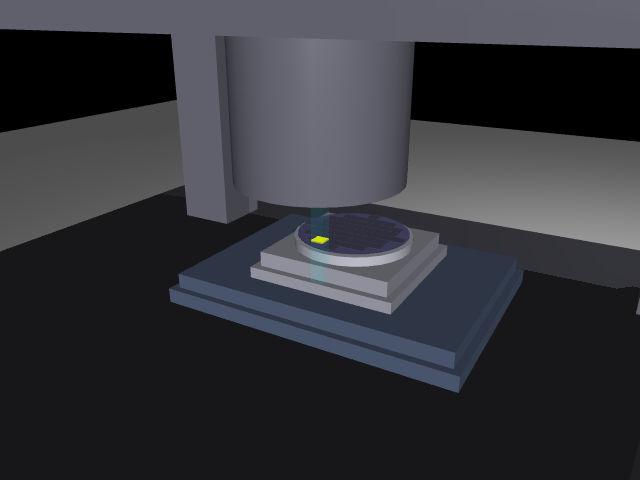
\includegraphics[width=\textwidth]{scanning_3d.png}
    \caption{Screenshot of the MuJoCo simulation in the midst of the scanning motion, showing the wafer and the optics chain under the metrology frame}
    \label{fig:scanning_simulation}
\end{figure}

To successfully adapt our planar reduction of the reference model~\cite{Al-Rawashdeh2022_Caracterization} into MuJoCo's multibody solver, two numerical adaptations are in order: 

\begin{enumerate}
    \item Native joint damping against absolute velocity would exert artificial drag ($K_V/K_P = 10$\,mm per m/s) during cruise, so we apply the velocity gain $K_V$ to the tracking-error velocity $(\dot{r} - \dot{y})$ within the control loop to represent the frictionless air bearings.

    \item Actuators transmit reaction forces to the parent body by default, so we apply reaction cancellation to the base frame at each integration step to represent balance masses used to absorb long-stroke reaction forces~\cite{Butler2011_PositionControl}, which the analytical model~\cite{Al-Rawashdeh2022_Caracterization} represents as external stage forces.
\end{enumerate}

Synchronized scanning motion is commanded with nominal cruise velocities of $v_{w,\mathrm{scan}} = 0.8$\,m/s and $v_{r,\mathrm{scan}} = 3.2$\,m/s. Under acceleration transients up to $a_{w,\max} = 20$\,m/s$^2$, this setup captures the full-state dynamic interactions derived in Section~\ref{sec:model_dynamics}.

Baseline control configurations (such as Case~1 in~\cite{Al-Rawashdeh2022_Caracterization}) are realized on this plant by disabling active fine-stage feedback loops.

\section{Reference Trajectory Generation}\label{sec:methodology_trajectories}

The trajectories commanded to the stages are \textbf{fourth-order profiles}: piecewise-polynomial motions in which position, velocity, acceleration, and jerk are all continuous, and the fourth derivative --- the \textit{snap} --- switches between $\pm s_{\max}$ and zero~\cite{Lambrechts2003_Trajectories}. Within each segment the position evolves as
\begin{equation}
    p(t) = p_0 + v_0 t + \frac{a_0}{2}t^2 + \frac{j_0}{6}t^3 + \frac{s}{24}t^4,
    \label{eq:fourth_order_poly}
\end{equation}
where ($p_0$, $v_0$, $a_0$, $j_0$) are the boundary conditions inherited from the previous segment and $s \in \{-s_{\max}, 0, +s_{\max}\}$. A symmetric point-to-point motion consists of fifteen such segments, arranged so that none of the kinematic bounds ($v_{\max}$, $a_{\max}$, $j_{\max}$, $s_{\max}$) is exceeded.

We implement an analytical trajectory generator that structures the motion profile across fifteen segments (seven per acceleration ramp) where snap is held constant. Physical limitations are addressed by the following considerations from~\cite{Lambrechts2003_Trajectories}:
\begin{itemize}
    \item When the jerk plateau cannot be reached, the effective jerk reduces to $\sqrt{a_{\max} s_{\max}}$
    \item If the acceleration limit is unreachable, then the effective acceleration follows from the corresponding quadratic equation; if the jerk phase collapses as well, the snap-phase duration instead follows from a cube-root solve
    \item If the total travel distance is too short to accommodate the required transition ramps, then the cruise velocity is iteratively reduced via bisection.
\end{itemize}
To streamline the trials, this same algorithmic structure is used to derive the lower order profiles: i.e., a second-order, acceleration-bounded trapezoidal profile and a third-order, seven-segment jerk-bounded S-curve.

The order of the motion profile determines the high-frequency content of the force commanded to initiate such motion: a second-order profile demands instantaneous jumps in acceleration, while a third-order profile is discontinuous in jerk~\cite{Dong2023_SCurve}, so both inject energy across a broad frequency band. A fourth-order trajectory, whose snap is bounded as noted above, is reported to roll off the excitation spectrum at $-80$\,dB per decade~\cite{Lambrechts2003_Trajectories} --- a theoretical asymptotic for constant-snap profiles, not separately verified spectrally in this work --- reducing the response of poorly damped structural modes such as those of the end-effectors, the reticle and the wafer. The settling period after each step~\cite{Lambrechts2003_Trajectories, Al-Rawashdeh2023_Trajectories} is thereby minimized, which is essential for the constant-velocity scanning phase, where ideally no force beyond the viscous terms is present.

\section{Stage Feedback Control}\label{sec:methodology_control}

The stage controllers are evaluated across four incremental configurations, following~\cite{Al-Rawashdeh2022_Caracterization}. Each setup introduces a specific feedforward or feedback component to isolate its impact on exposure performance in Chapter~\ref{ch:experiments}.

% (collocated long-stroke control)
In Case 1, each long-stroke stage is regulated in closed loop by a collocated PD controller acting on the long-stroke encoder $y_c(t)$:
\begin{equation}
    u(t) = K_P\, e(t) + K_V\, \dot{e}(t),
    \label{eq:case1_servo}
\end{equation}
where $e(t) = r(t) - y_c(t)$ is the long-stroke tracking error, with gains $K_P = 10^7$\,N/m and $K_V = 10^5$\,N$\cdot$s/m. Position and velocity are read from the long-stroke stage rather than the end-effector because non-collocated control through the lightly damped reticle coupling ($\zeta \approx 0.04$) destabilizes the loop. Consequently, the lag between the long-stroke stage and the end-effector remains uncompensated and appears directly in the synchronization error. On this frictionless plant, this lag is dominated by its acceleration-proportional component: servo deflection $m\,a/K_P$ and quasi-static coupling stretch $m_d\,a/K$ carrying the downstream mass $m_d$. This configuration serves as the baseline validated in Experiment~1 (Section~\ref{sec:exp_case1}).

% (collocated long-stroke control)
Since both lag components are functions of the known reference kinematics, in Case 2 they are cancelled by commanding the long stroke \textit{ahead} of the reference:
\begin{equation}
    r_{LS}(t) = r(t) - \big(\ell_v\, \dot{r}(t) + \ell_a\, \ddot{r}(t)\big),
    \label{eq:lag_ff}
\end{equation}
so that the end-effector may land on the desired position. The coefficients ($\ell_v$, $\ell_a$) for each chain are identified by performing iterative least-squares regressions on the end-effector lag with respect to reference velocity and acceleration. Each resulting fit is added to the feedforward control loop while subsequent passes repeat the regression on the remaining residuals. Three iterations are required to prevent post-acceleration coupling vibrations from skewing the quasi-static fit.This is a model-free equivalent to the spring-compensation configuration of the reference study~\cite{Al-Rawashdeh2022_Caracterization}.
%, and requires no additional hardware or sensing. What the fit cannot represent --- and what remains after Case 2 --- is precisely that dynamic transient, which motivates the fine-stage feedback below. This is the model-free counterpart of the spring-compensation configuration of the reference study, and requires no additional hardware or sensing.

% (fine-stage feedback)
The error remaining after feedforward is a non-repeatable transient response that can only be suppressed through feedback. Thus, in Case 3, the short-stroke stage of each chain implements a closed position loop on the end-effector error $e_f(t)$, commanding the short-stroke actuator directly. In actual step-and-scan systems, this measurement is readily available from interferometry, as required for exposure metrology. Case 3a uses a linear PI law with anti-windup, whereas Case 3b replaces the linear integrator with a Hybrid Integrator--Gain System (HIGS)~\cite{Heertjes2025_NonlinearControl}, given by:
\begin{equation}
    \dot{x}_1 = \omega_h\, e_f \quad \text{while } e_f\, x_1 \geq x_1^2 / k_h,
    \qquad x_1 = k_h\, e_f \quad \text{otherwise},
    \label{eq:higs}
\end{equation}
with output $u_f = k_p e_f + \omega_i \int x_1\, dt$. By resetting its state to the gain line $k_h e_f$ whenever the sector condition is violated, the HIGS element provides integral action with roughly $38^\circ$ less phase lag than a linear integrator, relaxing the overshoot-versus-stiffness limitation of linear designs --- the property that motivates nonlinear integrators for wafer stages. Both fine loops saturate at the physical travel of the short stroke, with conditional integration preventing windup during large transients. The loop gains are tuned empirically over a grid up to the stability boundary of the simulated plant: the PI loop uses $k_p = 16$, $k_i = 480$\,s$^{-1}$, and the HIGS loop $k_p = 16$, $\omega_i = 2\pi \cdot 200$\,rad/s, $\omega_h = 2\pi \cdot 80$\,rad/s, $k_h = 1$; one step further in gain destabilizes both loops against the $180$\,Hz flexible-chain modes. The HIGS element sustains an integrator frequency roughly $42\times$ above the PI's equivalent $k_i/k_p$ before reaching that boundary --- the phase advantage of the nonlinear integrator expressed as usable gain. The fine-stage authority is ultimately bounded by the short-stroke actuator's own velocity loop (pole at $K_P/K_V = 100$\,rad/s), a structural property of this generic replication that Chapter~\ref{ch:experiments} quantifies.

\section{Population-Based Trajectory Search}\label{sec:methodology_pso}

The optimization problem~\eqref{eq:problem} is searched with particle swarm optimization (PSO) over the four kinematic bounds. Each particle holds a position $\mathbf{x} = (v_{\max}, a_{\max}, j_{\max}, s_{\max})$ and is updated by the standard rule
\begin{equation}
    \mathbf{u}_{k+1} = \omega\, \mathbf{u}_k + c_1 r_1 (\mathbf{p}_k - \mathbf{x}_k) + c_2 r_2 (\mathbf{g}_k - \mathbf{x}_k), \qquad \mathbf{x}_{k+1} = \mathbf{x}_k + \mathbf{u}_{k+1},
    \label{eq:pso}
\end{equation}
with inertia $\omega = 0.6$, cognitive and social weights $c_1 = c_2 = 1.4$, velocities clamped to $\pm 0.5$ of the search-box span per dimension, and positions clipped to the search box. Evaluating one particle runs the full step-and-scan sequence over the wafer under the candidate trajectory, converts the per-die exposure indices into a wafer map, and prices the map. Two cost definitions are compared as the scenarios E3 and E4 of the evaluation plan: a conventional servo cost (the wafer-average exposure MSD, normalized by the failure threshold) and the yield-aware cost built on the CNN. For the latter, the weighted form~\eqref{eq:cost} is instantiated as
\begin{equation}
    \mathcal{J}_{map} = \big(1 - P_{none}\big) + \sum_{c\, \in\, \mathcal{C}_{ood}} P_c,
    \label{eq:cost_corrected}
\end{equation}
where $\mathcal{C}_{ood}$ is the set of classes that scanner motion cannot plausibly produce. The first term prices any departure from a clean map, so that the optimizer can spend an \textit{acceptable-pattern} yield loss when it is worth it; the second is a hard wall that keeps it from cheapening the wafer into a morphology the classifier attributes to non-scanner mechanisms. Both scenarios share a throughput reward $\mathcal{J} = \mathcal{J}_{map} + \gamma\, T_{wafer}/T_{ref}$ with $\gamma = 1$ and $T_{ref} = 15$\,s, so that a faster wafer is cheaper and the search trades cycle time against the map cost rather than merely respecting a budget; $T_{wafer}$ follows from the scan-profile duration, the settling budget, and the die count.

\section{From Synchronization Error to Wafer Maps}\label{sec:methodology_cnn}

The link between trajectory parameters and yield is established in three steps: the simulated synchronization error is aggregated per die, the resulting pass/fail pattern forms a simulated wafer map, and a convolutional neural network classifies that map into a defect-morphology class.

The CNN classifier is trained on WM-811K~\cite{Wu2015_WM811K}, a public dataset of 811{,}457 wafer maps collected from real fabrication lines, of which 172{,}950 carry a manually assigned failure label. Each map is a grid of dies marked as pass or fail, annotated with one of nine morphology classes: \textit{none}, \textit{Center}, \textit{Donut}, \textit{Edge-Loc}, \textit{Edge-Ring}, \textit{Loc}, \textit{Near-full}, \textit{Random}, and \textit{Scratch}. The labelled maps are split 80/20 with class stratification, and every map is resized to $64 \times 64$ cells to give the network a uniform input.

The network architecture comprises three convolutional blocks (16, 32, and 64 filters of size $3\times3$, each followed by ReLU activation and $2\times2$ max-pooling) and two fully connected layers (128 hidden units with dropout of 0.5, and a 9-way softmax output). It is trained for 5 epochs with the Adam optimizer (learning rate $10^{-3}$, batch size 32) under a cross-entropy loss, retaining the weights with the highest hold-out accuracy.

To generate simulated maps, for each die scanned in simulation, the synchronization error recorded during its exposure is reduced to a scalar criterion --- either the maximum tracking error or the MA/MSD pair of Chapter~\ref{ch:control_objectives} --- and compared against a threshold to declare the die good or failing. The resulting grid, arranged in the same encoding as WM-811K (background, pass, fail), is resized to $64\times64$ and presented to the CNN, which returns the probability distribution $P_c$ used by the cost function~\eqref{eq:cost}.

For validation, a physically meaningful trajectory-to-defect mapping must activate only the classes plausibly caused by scanner motion: \textit{none}, \textit{Scratch}, \textit{Edge-Loc}, and \textit{Random}. The remaining classes correspond to etching, cleaning, and deposition signatures; if simulated maps systematically activated them, the mapping --- not the machine --- would be at fault. This criterion, together with the requirement that the cost shift reproducibly under sweeps of $(v_{\max}, a_{\max}, j_{\max}, s_{\max})$, defines what constitutes a successful validation in Chapter~\ref{ch:experiments}.


\def\baselinestretch{1}

\chapter{Experiments and Results}\label{ch:experiments}

\def\baselinestretch{1.66}

\section{Introduction}\label{sec:experiments_introduction}

This chapter reports the experimental campaign carried out over the simulation framework of Chapter~\ref{ch:methodology}. Experiment 1 validates the simulated machine against the published Case 1 study it derives from, establishing the dynamic behavior of the plant without fine stages. Experiment 2 trains and evaluates the convolutional network on the WM-811K dataset, establishing the classifier half of the pipeline. Experiment 3 connects the two: it verifies that disturbances injected into the simulation produce wafer-map signatures the CNN can react to, and that sweeping the kinematic bounds $(v_{\max}, a_{\max}, j_{\max}, s_{\max})$ shifts the exposure error --- and therefore the defect map --- reproducibly. Experiment 4 climbs the control ladder of Section~\ref{sec:methodology_control}: lag-compensation feedforward, fine-stage PI, and the nonlinear HIGS loop, quantifying the contribution of each. Experiment 5 is the central demonstration of the thesis premise: as the settling budget shrinks, trajectory-induced failures emerge as a spatially structured, scanner-plausible pattern, and the yield-aware cost traces the throughput--yield transition. Experiment 6 runs the optimization scenarios E3 and E4, comparing the conventional servo cost against the CNN cost inside the same particle-swarm search over the exact snap-bounded profile family. Experiment 7 crosses profile order with controller quality, quantifying whether trajectory smoothness matters when the controller is poor and how much it is worth when the controller is good. A closing secondary study evaluates the recurrent surrogate model. All results reported below are outputs of the actual scripts and trained models of this project; where a result falls short of the criterion set in Chapter~\ref{ch:control_objectives}, this is stated and analyzed rather than omitted.

\section{Experiment 1: Reproduction of the Case 1 Study}\label{sec:exp_case1}

The first experiment reproduces Case 1 of the characterization study by Al-Rawashdeh et al.~\cite{Al-Rawashdeh2022_Caracterization}: planar step-and-scan motion of the wafer and reticle chains \textit{without} fine stages, under the collocated PID-plus-feedforward controller of Section~\ref{sec:methodology_control}. The purpose is twofold: to verify that the simulation reproduces the qualitative conclusions of the reference study, and to quantify how far a coarse-only machine falls from the exposure specifications, which motivates everything that follows.

The reduced two-body-per-chain model is integrated over a four-die exposure sequence (dies of $32 \times 32$\,mm$^2$ in a single row) with the baseline trajectory parameters $v_{w,scan} = 0.8$\,m/s, $a_{w,\max} = 20$\,m/s$^2$, $j_{\max} = 1600$\,m/s$^3$: the scan profile lasts 145\,ms with a constant-velocity cruise between 52.5 and 92.5\,ms, each step takes 82.2\,ms, and the whole sequence spans 1.727\,s. The reticle moves at $3.2$\,m/s with $a_{r,\max} = 80$\,m/s$^2$ in the opposite direction. Figure~\ref{fig:exp1_trajectories} shows the commanded references, and Figure~\ref{fig:exp1_tracking} the resulting tracking and synchronization errors with the exposure windows highlighted.

\begin{figure}[htbp]
    \centering
    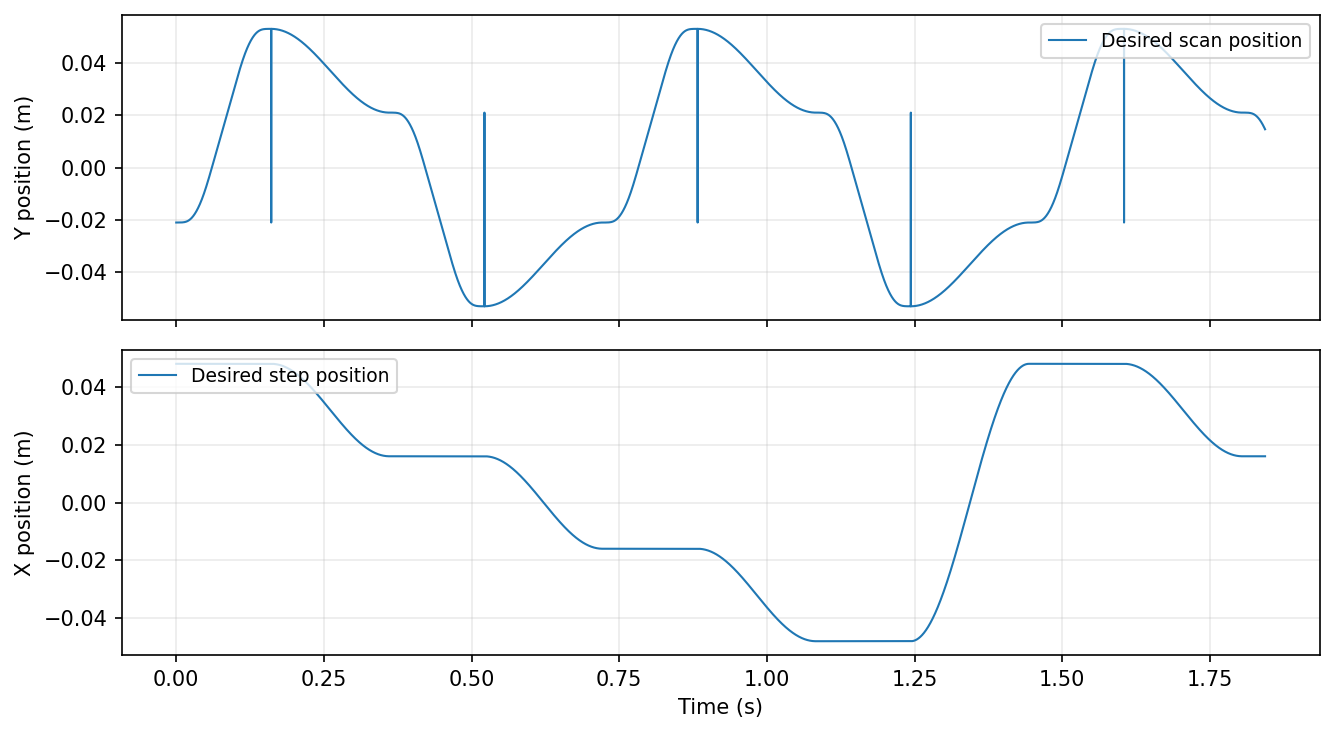
\includegraphics[width=0.85\textwidth]{case1_fig12_trajectories.png}
    \caption{Commanded step-and-scan references for the wafer stage ($x$: stepping, $y$: scanning) over the four-die sequence.}
    \label{fig:exp1_trajectories}
\end{figure}

\begin{figure}[htbp]
    \centering
    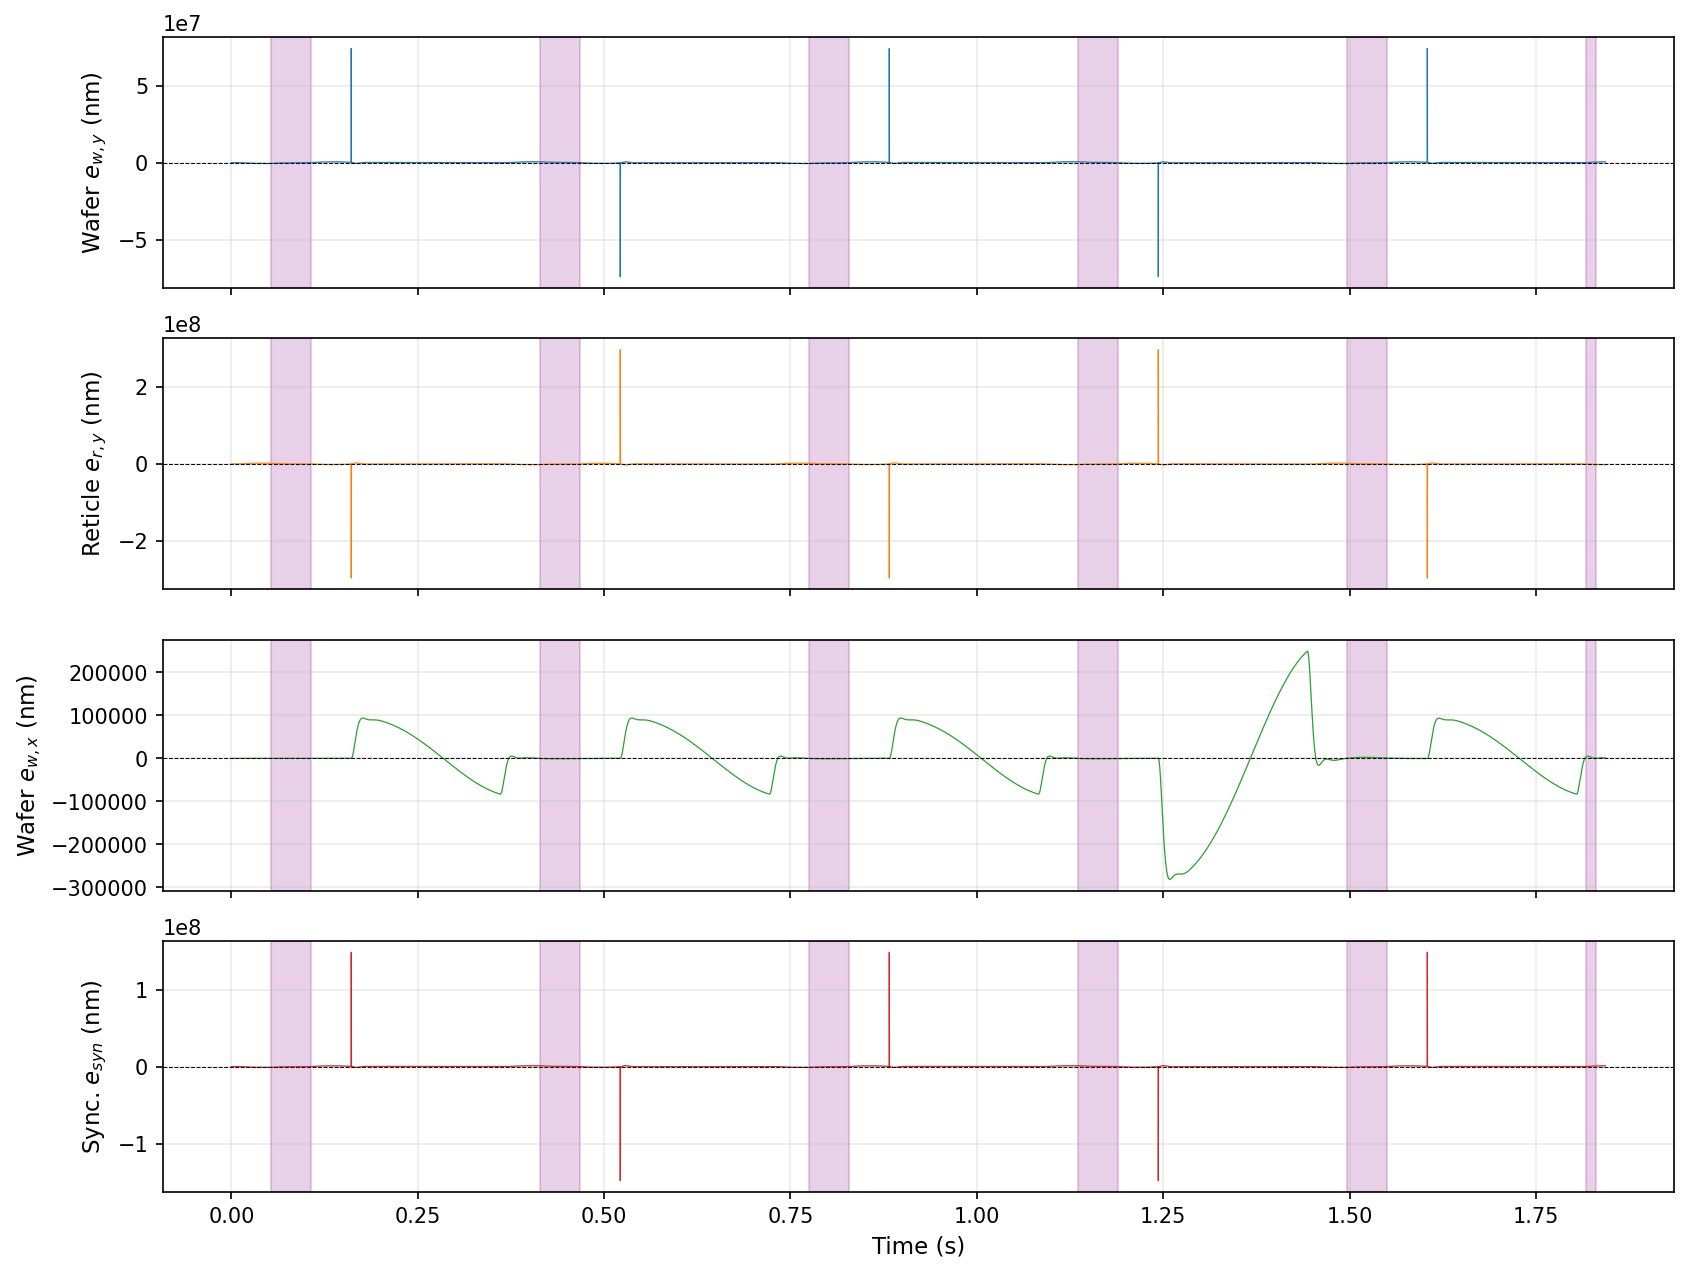
\includegraphics[width=\textwidth]{case1_tracking_errors.png}
    \caption{Wafer, reticle, and synchronization errors during the four-die sequence. Shaded bands mark the exposure windows.}
    \label{fig:exp1_tracking}
\end{figure}

The dynamic structure of the simulated machine matches the reference study. The wafer chain exhibits its two-mass resonance at 190.3\,Hz with a well-damped coupling ($\zeta = 0.70$), while the reticle chain resonates at 131.4\,Hz with $\zeta = 0.044$: the reticle end-effector is lightly damped, and non-collocated feedback through this coupling is unstable, which forces the collocated architecture and leaves the coupling lag uncompensated. During the acceleration ramps this lag reaches its quasi-static value $\Delta = m_e a / K$: $15.9$\,\textmu m for the wafer end-effector ($10.7$\,kg at $20$\,m/s$^2$) and $133.5$\,\textmu m for the reticle end-effector ($10.54$\,kg at $80$\,m/s$^2$), leaving a net quasi-static synchronization error of about $-17.4$\,\textmu m during the ramps (Figure~\ref{fig:exp1_velocity_lag}).

\begin{figure}[htbp]
    \centering
    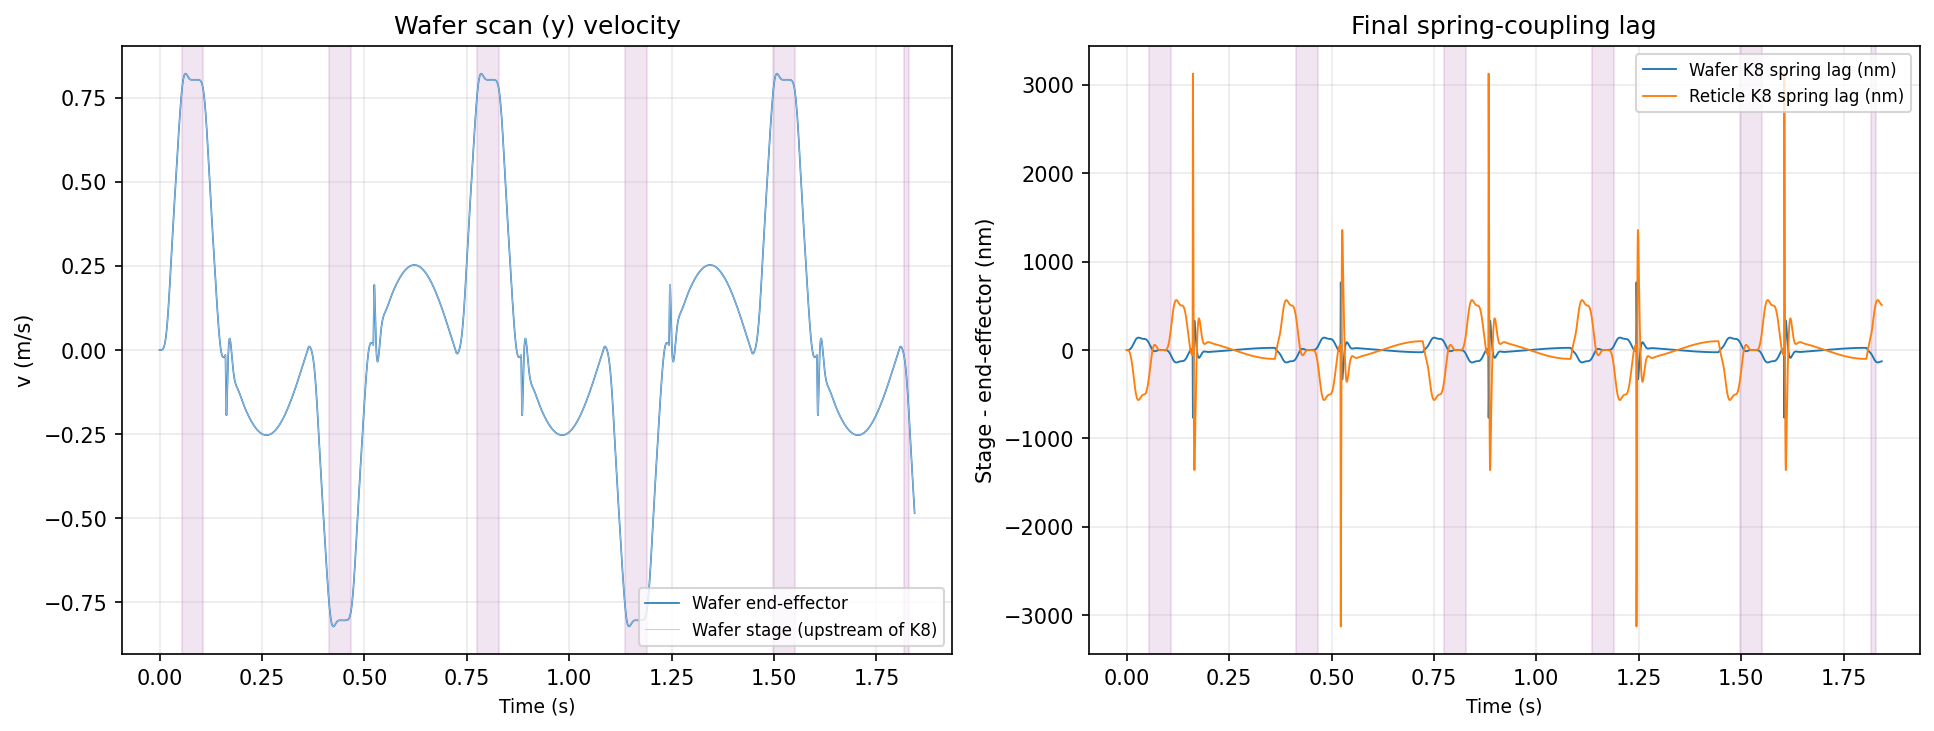
\includegraphics[width=\textwidth]{case1_velocity_lag.png}
    \caption{Stage velocities and spring-coupling lag during the scan. The reticle end-effector, four times faster and an order of magnitude more softly coupled, dominates the synchronization error.}
    \label{fig:exp1_velocity_lag}
\end{figure}

Inside the exposure windows --- where only the residual oscillation of the lightly damped reticle mode remains --- the performance indices evaluate to
\begin{equation}
    \mathrm{MA}_{syn} \in [-985.3,\ +985.2]\ \mathrm{nm}, \qquad
    \max \mathrm{MSD}_{syn} = 427.8\ \mathrm{nm},
    \label{eq:exp1_ma_msd}
\end{equation}
against the specifications $\mathrm{MA} \in [-1.25, +2]$\,nm and $\mathrm{MSD} \leq 7$\,nm of Chapter~\ref{ch:control_objectives}. Figure~\ref{fig:exp1_ma_msd} shows both indices over the sequence and Figure~\ref{fig:exp1_zoom} the detail of the first exposure window.

\begin{figure}[htbp]
    \centering
    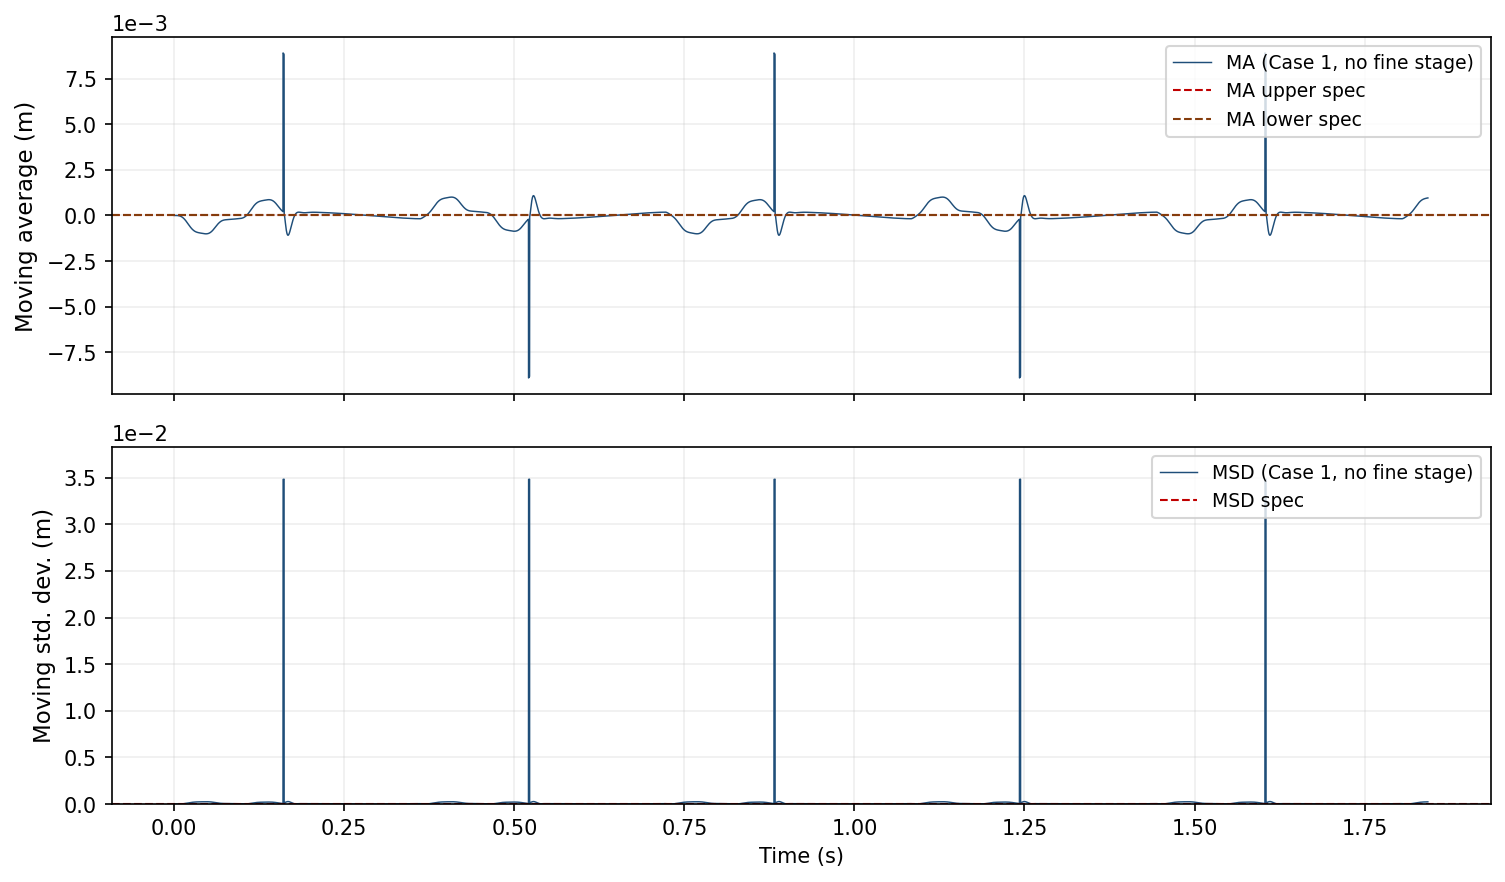
\includegraphics[width=\textwidth]{case1_fig14_ma_msd.png}
    \caption{MA and MSD performance indices of the synchronization error over the four-die sequence.}
    \label{fig:exp1_ma_msd}
\end{figure}

\begin{figure}[htbp]
    \centering
    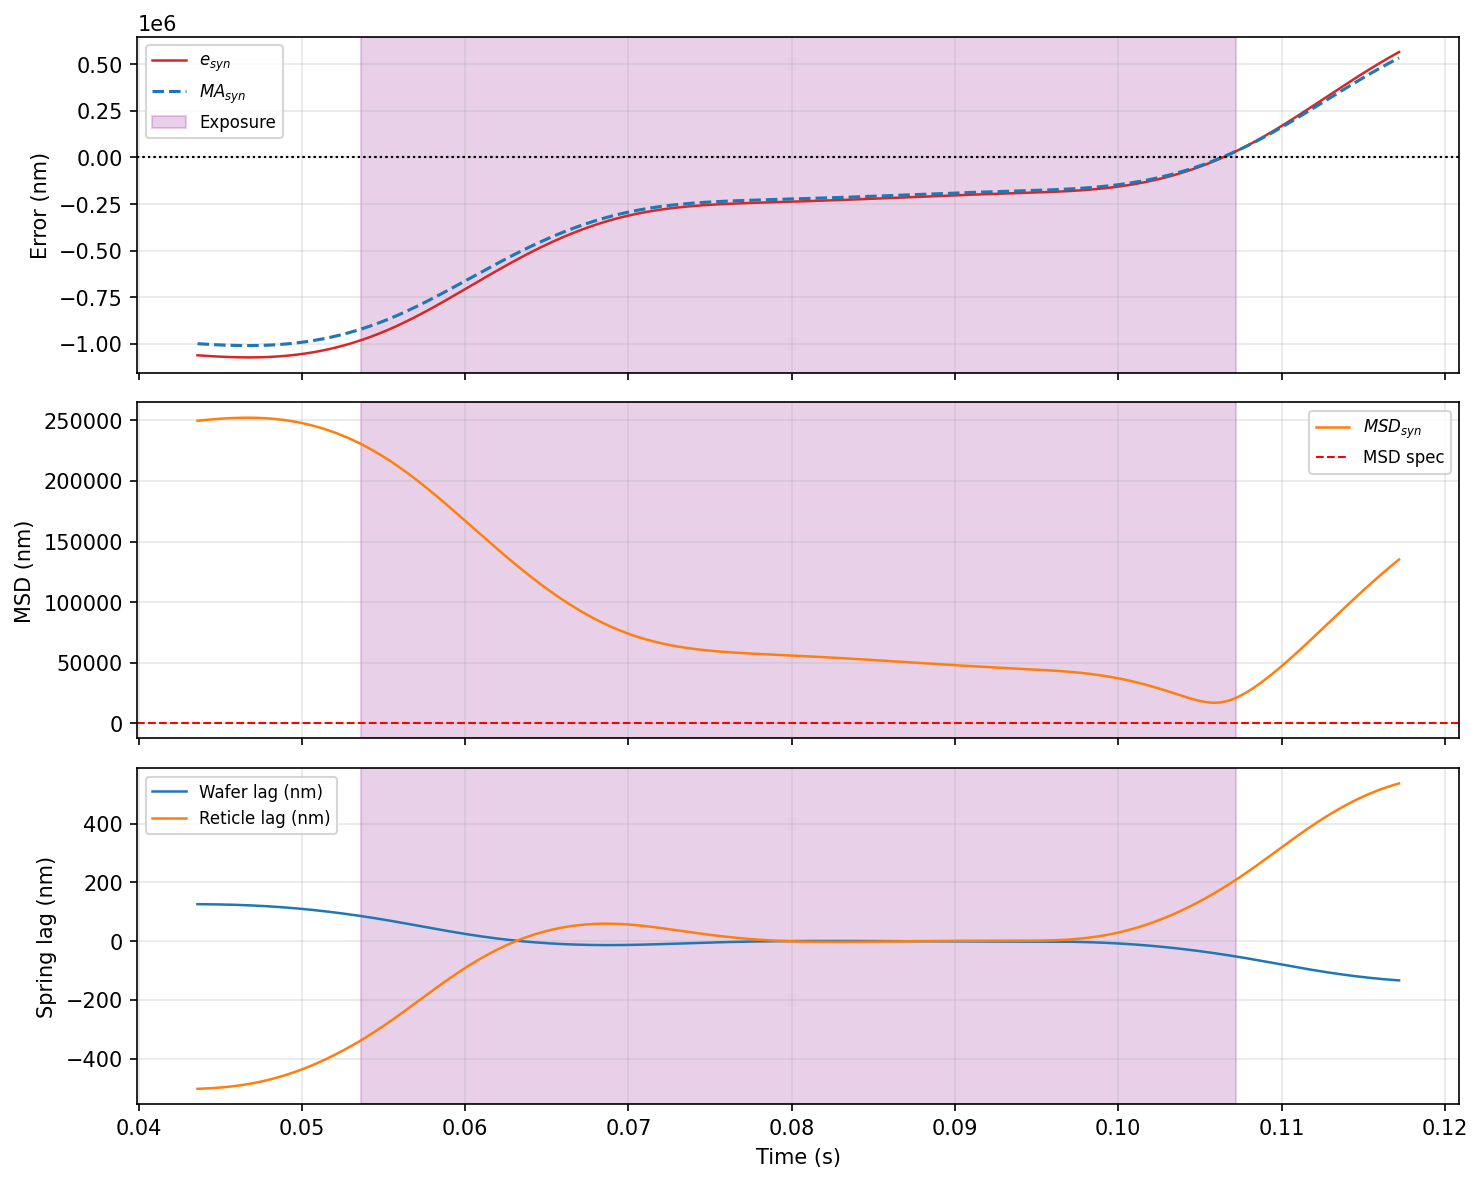
\includegraphics[width=\textwidth]{case1_exposure_zoom.png}
    \caption{Detail of the first exposure window: synchronization error, MA, MSD, and coupling lag.}
    \label{fig:exp1_zoom}
\end{figure}

The conclusion of the experiment is the same as that of the reference study: a machine without fine stages misses the exposure specification by nearly three orders of magnitude, with the error dominated by the residual 131\,Hz oscillation of the reticle end-effector excited during the acceleration ramps. This is the error mechanism that trajectory shaping acts upon --- gentler kinematic bounds inject less energy at the resonance --- and the mechanism that the remaining experiments quantify at the wafer-map level.

\section{Experiment 2: CNN Training and Evaluation on WM-811K}\label{sec:exp_cnn}

The second experiment trains the classifier of Section~\ref{sec:methodology_cnn} and evaluates it on held-out data. Of the 811{,}457 maps in WM-811K, the 172{,}950 maps carrying a failure label are used; the stratified 80/20 split leaves 34{,}590 maps for evaluation, never seen during training.

The network reaches an overall hold-out accuracy of \textbf{96.88\,\%} with a macro-averaged F1 score of 0.77. Table~\ref{tab:exp2_metrics} reports the per-class precision, recall, and F1, and Figure~\ref{fig:exp2_confmat} the row-normalized confusion matrix.

\begin{table}[htbp]
\centering
\caption{Per-class evaluation of the CNN on the WM-811K hold-out set (34{,}590 maps).}
\label{tab:exp2_metrics}
\begin{tabular}{lcccc}
\toprule
Class & Precision & Recall & F1 & Support \\
\midrule
none      & 0.98 & 1.00 & 0.99 & 29{,}486 \\
Center    & 0.95 & 0.90 & 0.92 & 859 \\
Donut     & 0.85 & 0.84 & 0.85 & 111 \\
Edge-Loc  & 0.87 & 0.75 & 0.80 & 1{,}038 \\
Edge-Ring & 0.94 & 0.99 & 0.97 & 1{,}936 \\
Loc       & 0.76 & 0.63 & 0.69 & 718 \\
Near-full & 0.96 & 0.80 & 0.87 & 30 \\
Random    & 0.87 & 0.76 & 0.81 & 173 \\
Scratch   & 0.00 & 0.00 & 0.00 & 239 \\
\midrule
accuracy  & \multicolumn{4}{c}{0.9688} \\
macro avg & 0.80 & 0.74 & 0.77 & 34{,}590 \\
\bottomrule
\end{tabular}
\end{table}

\begin{figure}[htbp]
    \centering
    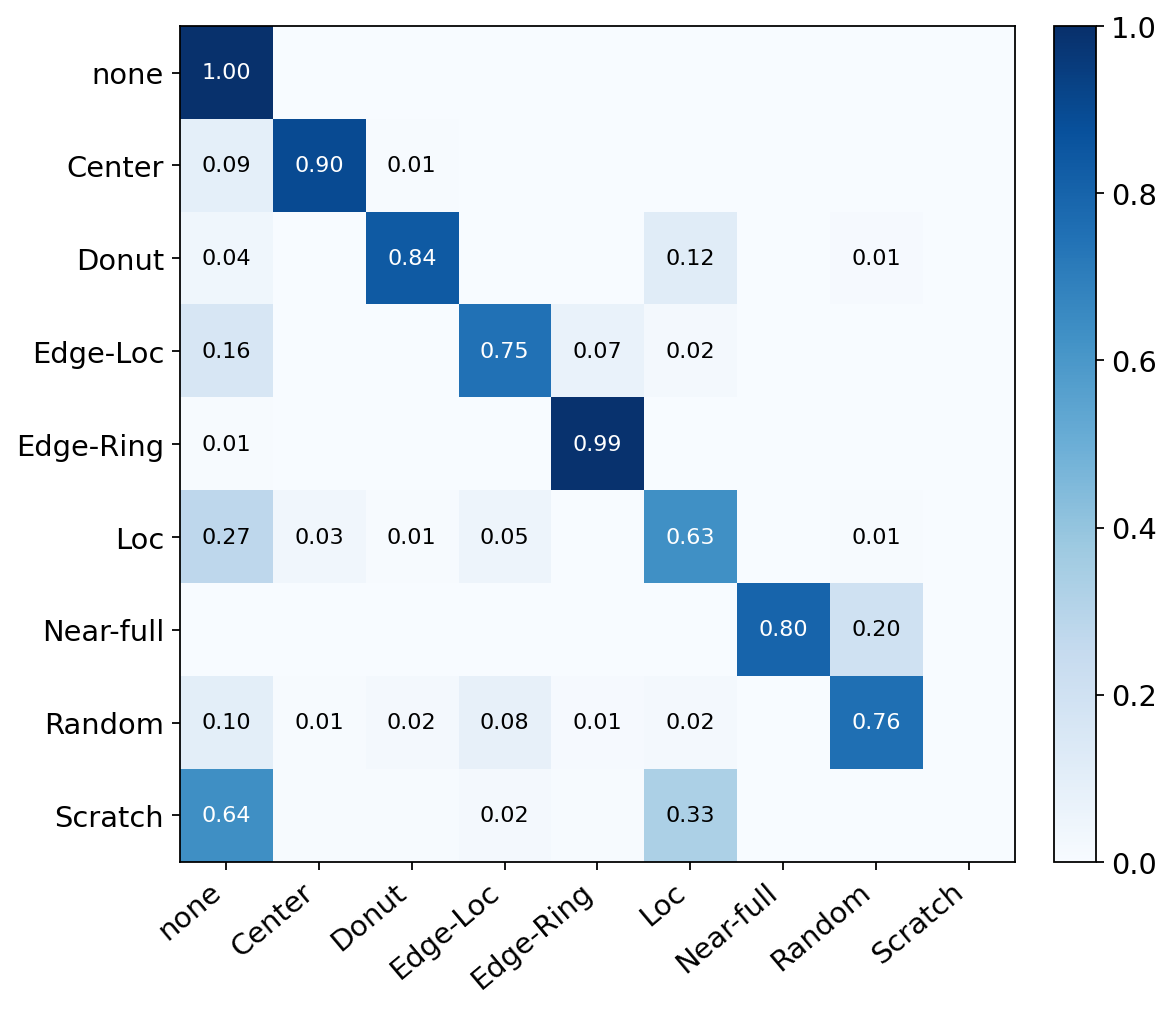
\includegraphics[width=0.75\textwidth]{confusion_matrix.png}
    \caption{Row-normalized confusion matrix of the CNN on the WM-811K hold-out set.}
    \label{fig:exp2_confmat}
\end{figure}

The matrix is strongly diagonal for eight of the nine classes. The exception is \textit{Scratch}, whose recall is zero: with 239 test samples against 29{,}486 \textit{none} samples, the cross-entropy objective is dominated by the majority classes and the network learns to absorb the thin-line morphology into neighboring classes. This is a known consequence of the severe class imbalance of WM-811K and matters here because \textit{Scratch} is one of the four scanner-plausible classes. Mitigation --- class-weighted loss, oversampling, or focal loss --- is deliberately deferred: it modifies only the training recipe of Experiment 2 and leaves the rest of the pipeline unchanged.

\section{Experiment 3: Trajectory-to-Defect Pipeline}\label{sec:exp_pipeline}

The third experiment exercises the full bridge of Section~\ref{sec:methodology_cnn} over the complete 300\,mm wafer (49 dies of $32\times32$\,mm$^2$) in the full MuJoCo model. Two campaigns are run: disturbance injection at fixed trajectory parameters, and a sweep of the kinematic bounds at fixed (zero) disturbance. Both campaigns operate under Case 1 control (long-stroke tracking only); Experiment 4 then upgrades the controller, and Experiments 5 and 6 run on top of the upgraded configuration.

A practical observation conditions both campaigns. In the Case 1 machine, the exposure-window MSD of the synchronization error sits between 33 and 230\,\textmu m depending on the trajectory --- roughly four orders of magnitude above the 7\,nm specification, consistently with Experiment 4's ladder baseline. An absolute threshold at the specification therefore marks every die of every wafer as failing and produces saturated, uninformative maps. Both campaigns consequently use criteria referenced to the unperturbed baseline of the same machine: what is measured is the \textit{relative} effect of the disturbance or of the trajectory parameters, not compliance with a specification that this machine configuration cannot reach.

\subsection{Disturbance signatures}\label{sec:exp_perturb}

Three disturbance types are injected as forces on the wafer end-effector while the baseline trajectory runs: broadband force noise on both axes (floor \textit{vibration}), a sustained bias force active while scanning dies near the wafer edge (\textit{drift}), and a sustained bias force active while scanning a single die column (\textit{scratch}). For every die, the synchronization error during the central third of the scan --- the constant-velocity cruise that contains the exposure --- is reduced to its mean and its maximum moving standard deviation. A die is marked as failing when its mean shifts by more than 100\,nm with respect to the same die in the unperturbed run, or when its MSD exceeds twice the baseline median; both criteria are immune to the constant geometric offset of the absolute coordinates. The resulting maps are classified by the CNN of Experiment 2.

This campaign uses a finer die grid than the sweep --- $16\times16$\,mm$^2$ dies, 241 per wafer --- so that line- and point-like patterns retain their morphology after resizing to the CNN input. Table~\ref{tab:exp3_perturb} and Figure~\ref{fig:exp3_perturb_maps} present the results.

\begin{table}[htbp]
\centering
\caption{Disturbance-injection campaign over 241 dies. Expected class refers to the scanner-plausible morphology the disturbance emulates.}
\label{tab:exp3_perturb}
\begin{tabular}{lcccc}
\toprule
Disturbance & Failing dies & Spatial pattern & Expected class & CNN prediction \\
\midrule
none        & 0/241   & clean wafer     & none      & none (97.2\,\%) \\
vibration   & 92/241  & scattered       & Random    & Center (60.1\,\%) \\
drift       & 105/241 & outer ring      & Edge-Ring / Edge-Loc & Donut (99.9\,\%) \\
scratch     & 15/241  & one die column  & Scratch   & Loc (63.1\,\%) \\
\bottomrule
\end{tabular}
\end{table}

\begin{figure}[htbp]
    \centering
    \begin{tabular}{cccc}
    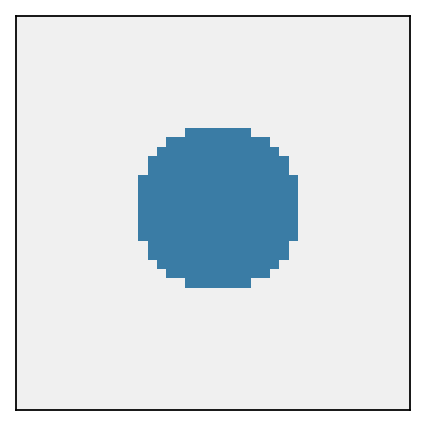
\includegraphics[width=0.22\textwidth]{perturb_map_none.png} &
    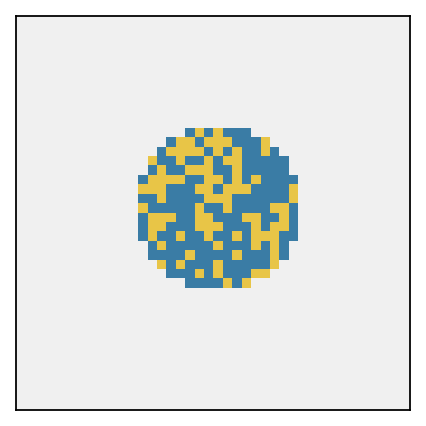
\includegraphics[width=0.22\textwidth]{perturb_map_vibration.png} &
    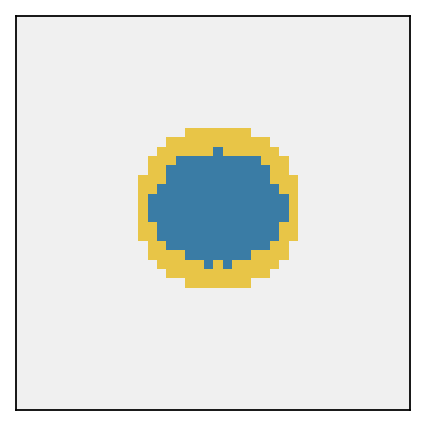
\includegraphics[width=0.22\textwidth]{perturb_map_drift.png} &
    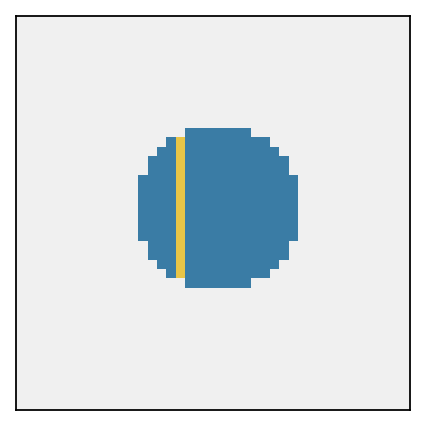
\includegraphics[width=0.22\textwidth]{perturb_map_scratch.png} \\
    (a) none & (b) vibration & (c) drift & (d) scratch \\
    \end{tabular}
    \caption{Simulated wafer maps under the four disturbance conditions (yellow: failing dies, blue: passing dies). The spatial signatures --- clean, scattered, ring, line --- correspond to the injected disturbances.}
    \label{fig:exp3_perturb_maps}
\end{figure}

The spatial half of the pipeline behaves as designed: the unperturbed wafer is clean and each disturbance produces a failing-die population of the expected shape and location --- scattered dies under force noise, an outer ring under the edge bias, and a single 15-die column under the column bias. The classification half is only partially aligned with the scanner-plausible target classes. The clean wafer is correctly assigned to \textit{none}, satisfying the first requirement of the validation criterion. The remaining assignments land on morphological neighbors rather than on the intended classes: the ring is read as \textit{Donut} --- a defensible reading, since the drift band covers an annulus wider than the one-die rim that characterizes \textit{Edge-Ring} in WM-811K --- the column is read as \textit{Loc}, the closest available class given that the classifier's \textit{Scratch} recall is zero (Experiment 2), and the scattered pattern, at a density of 38\,\% of the wafer, is absorbed into \textit{Center} rather than \textit{Random}. These deviations trace back to the classifier's minority-class weakness and to the density of the injected failures, not to the simulation half of the pipeline; they are taken up in the discussion of Section~\ref{sec:exp_discussion}.

\subsection{Kinematic-bound sweep}\label{sec:exp_sweep}

The second campaign fixes the disturbances at zero and sweeps the kinematic bounds around the baseline $(0.8\ \mathrm{m/s},\ 20\ \mathrm{m/s^2},\ 1600\ \mathrm{m/s^3},\ 10^5\ \mathrm{m/s^4})$: one aggressive configuration raises all four bounds, and four configurations relax one bound at a time; a conservative configuration relaxes all four. For every die the maximum moving-window MSD of the synchronization error during the scan is computed, a die fails when it exceeds the scaled threshold (the baseline median, 90\,\textmu m), and the map is classified by the CNN; the cost is the total probability assigned to the scanner-plausible defect classes.

Table~\ref{tab:exp3_sweep} summarizes the seven configurations. The median exposure MSD now responds monotonically to every one of the four kinematic bounds. Relative to the baseline (90\,\textmu m, 24 of 49 dies failing), raising all four bounds together drives it to 230\,\textmu m with the entire wafer failing, whereas relaxing any single bound lowers it: halving the acceleration brings the median to 77\,\textmu m, quartering the jerk to 72\,\textmu m, halving the velocity to 65\,\textmu m, tightening the snap to 49\,\textmu m, and the conservative configuration that gentles all four bounds to 33\,\textmu m --- each passing all but one die. Two points distinguish this sweep from a naive expectation. First, the snap bound is a live parameter: tightening it tenfold lowers the median MSD to 49\,\textmu m and lengthens the scan profile from 161 to 248\,ms, because the exact segment generator (Section~\ref{sec:methodology_trajectories}) imposes $s_{\max}$ directly rather than implying it from the ramp duration, so the fourth bound shapes the excitation spectrum as the other three do. Second, the velocity bound acts in the same direction as the others: halving $v$ lowers the median error, since the gentler ramp injects less energy into the flexible modes --- the accuracy gain of a slower scan is real, and it is precisely the counterweight to its throughput cost that the optimizer of Experiment 6 must resolve, the two effects pulling $v$ in opposite directions. Since the runs are deterministic, repeated execution reproduces these values exactly, satisfying the reproducibility half of the validation criterion.

\begin{table}[htbp]
\centering
\caption{Kinematic-bound sweep over the full 49-die wafer. $T_{scan}$ is the duration of one scan profile; the failure threshold is the baseline median MSD (90\,\textmu m); cost is the total CNN probability of the scanner-plausible defect classes.}
\label{tab:exp3_sweep}
\setlength{\tabcolsep}{0.14cm}
\begin{tabular}{lcccccccc}
\toprule
Config & $v$ & $a$ & $j$ & $s$ & $T_{scan}$ & med.\ MSD & Failing & CNN top class \\
 & [m/s] & [m/s$^2$] & [m/s$^3$] & [m/s$^4$] & [ms] & [\textmu m] & dies & (prob.) \\
\midrule
Aggressive   & 1.2 & 40 & 5000 & $5\times10^5$ & 112.6 & 230 & 49/49 & Center (1.000) \\
Baseline     & 0.8 & 20 & 1600 & $10^5$        & 160.8 & 90  & 24/49 & Center (0.841) \\
Tighter snap & 0.8 & 20 & 1600 & $10^4$        & 248.1 & 49  & 1/49  & none (0.991) \\
Half velocity& 0.4 & 20 & 1600 & $10^5$        & 162.9 & 65  & 1/49  & none (0.991) \\
Half accel.  & 0.8 & 10 & 1600 & $10^5$        & 226.3 & 77  & 4/49  & none (0.998) \\
Quarter jerk & 0.8 & 20 & 400  & $10^5$        & 223.5 & 72  & 1/49  & none (0.991) \\
Conservative & 0.2 & 5  & 200  & $5\times10^3$ & 333.6 & 33  & 1/49  & none (0.991) \\
\bottomrule
\end{tabular}
\end{table}

\begin{figure}[htbp]
    \centering
    \begin{tabular}{ccc}
    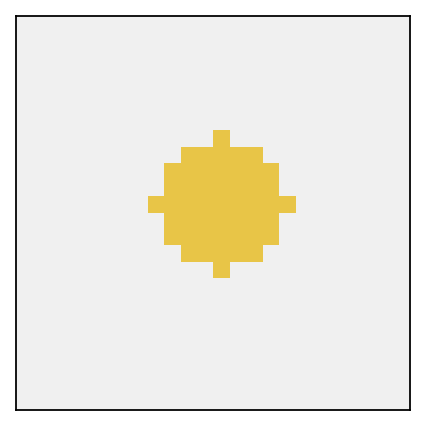
\includegraphics[width=0.28\textwidth]{sweep_map_aggressive.png} &
    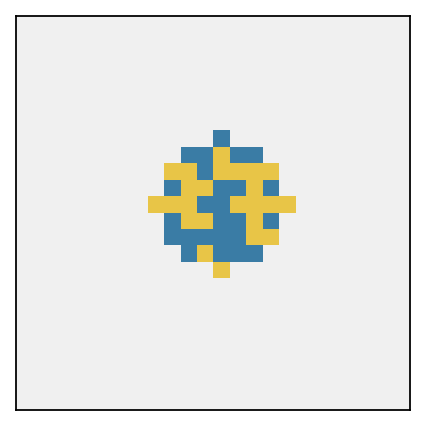
\includegraphics[width=0.28\textwidth]{sweep_map_baseline.png} &
    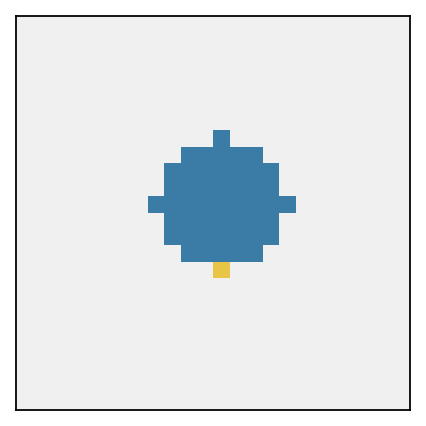
\includegraphics[width=0.28\textwidth]{sweep_map_conservative.png} \\
    (a) aggressive & (b) baseline & (c) conservative \\
    \end{tabular}
    \caption{Simulated wafer maps under the scaled MSD criterion for three points of the sweep (yellow: failing dies, blue: passing dies). The failing-die population collapses from full-wafer to a single die as the kinematic bounds are relaxed.}
    \label{fig:exp3_sweep_maps}
\end{figure}

The wafer maps (Figure~\ref{fig:exp3_sweep_maps}) and their classification expose a property of the cost function that matters for the optimization stage. Configurations that pass have $P_{none} = 0.991$ and a residual defect-class cost of 0.0056; but the saturated maps of the aggressive and baseline configurations concentrate essentially all probability in \textit{Center} --- a class outside the scanner-plausible subset --- so the cost restricted to plausible classes evaluates to zero exactly where the wafer is worst. A dense, wafer-wide failure pattern has no thin-line or scattered morphology left for the CNN to recognize. For the optimizer of Eq.~\eqref{eq:problem} this dictates either complementing the cost with the $1 - P_{none}$ term or penalizing any activation of the non-plausible classes as an out-of-domain signal; both preserve the CNN as the cost backbone while removing the blind spot.

\section{Experiment 4: Climbing the Control Ladder}\label{sec:exp_ladder}

The pipeline experiments above ran under Case 1 control, where the exposure error is millimetre-scale and the failure thresholds had to be scaled accordingly. This experiment adds, one at a time, the mechanisms of Section~\ref{sec:methodology_control} that make fourth-order trajectories trackable, and measures the contribution of each on the baseline trajectory over a four-die row in the full simulation model. Table~\ref{tab:exp4_ladder} reports the cruise-window indices of the offset-corrected synchronization error; Figure~\ref{fig:exp4_ladder} shows the error traces.

\begin{table}[htbp]
\centering
\caption{Controller ladder on the baseline trajectory (cruise-window indices of $e_{syn}$, worst die).}
\label{tab:exp4_ladder}
\begin{tabular}{lcc}
\toprule
Configuration & max $|\mathrm{MA}|$ & max MSD \\
\midrule
Case 1: long-stroke PID only          & 817\,\textmu m   & 19.7\,\textmu m \\
Case 2: + lag-compensation FF          & 69.1\,\textmu m  & 4.72\,\textmu m \\
Case 3a: + fine-stage PI               & 1.10\,\textmu m  & 0.111\,\textmu m \\
Case 3b: + fine-stage HIGS             & 0.873\,\textmu m & 0.096\,\textmu m \\
\bottomrule
\end{tabular}
\end{table}

\begin{figure}[htbp]
    \centering
    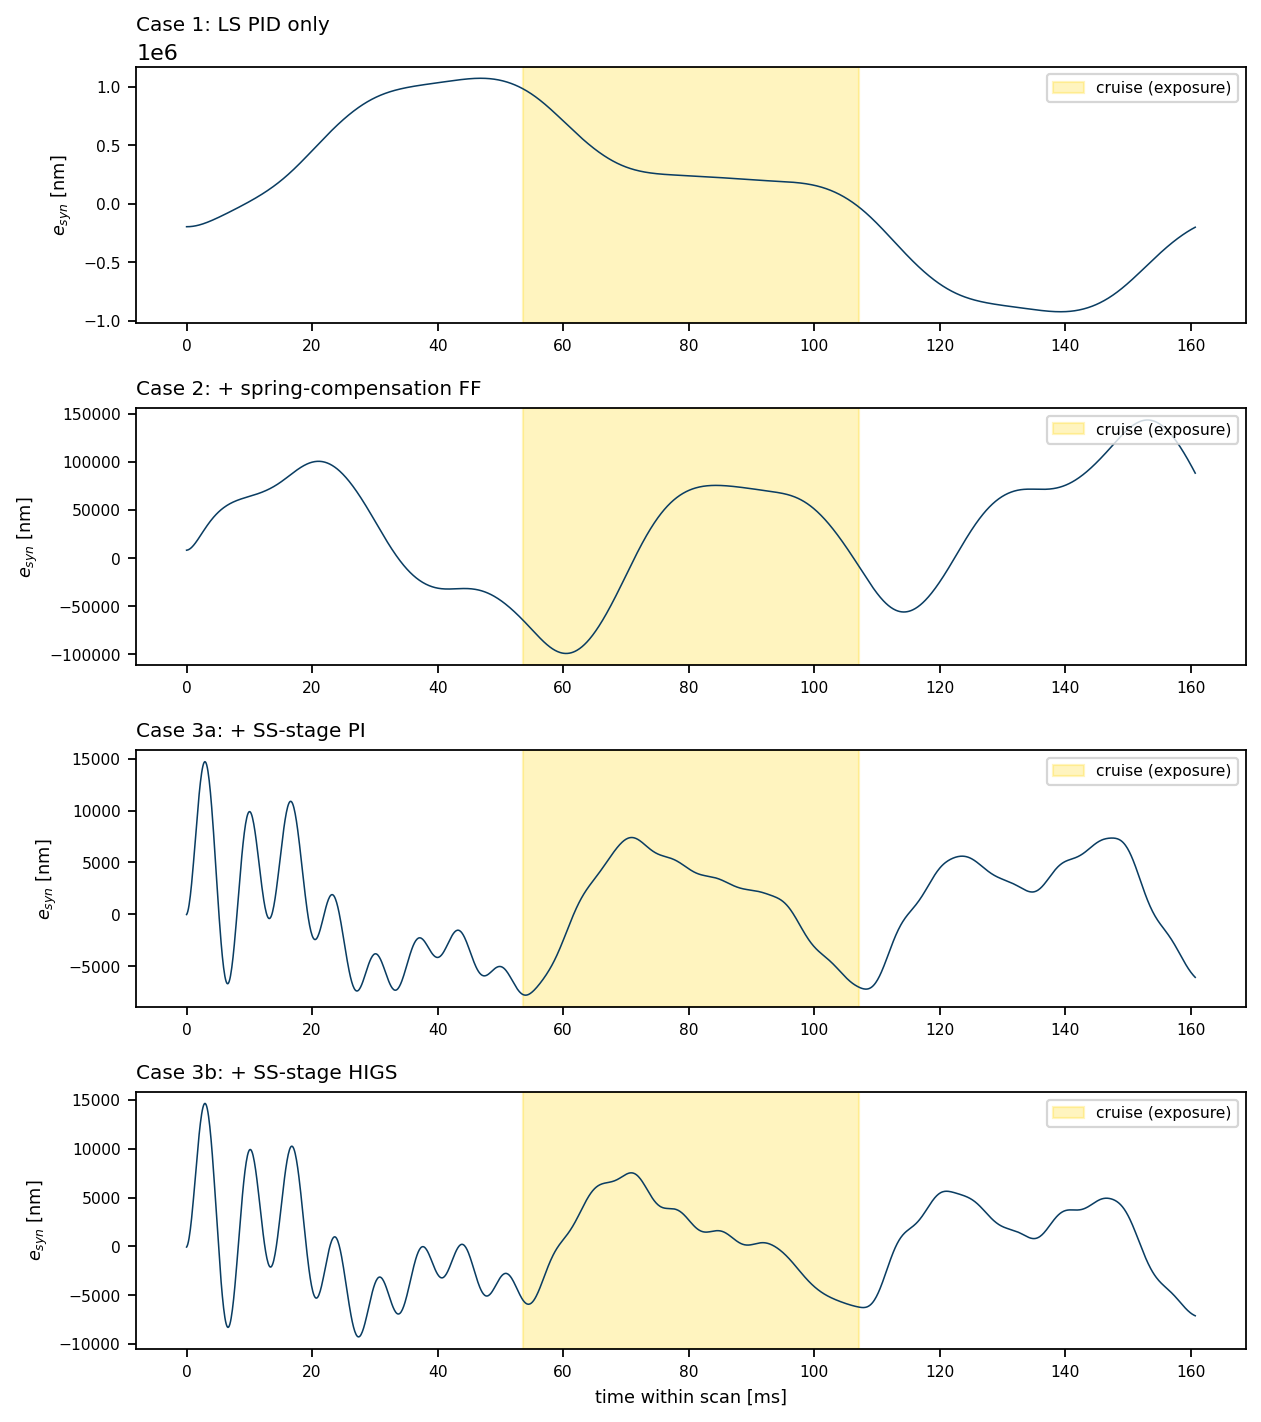
\includegraphics[width=0.9\textwidth]{controllers_esyn.png}
    \caption{Synchronization error during one scan under the four control configurations. Shaded band: cruise (exposure) segment.}
    \label{fig:exp4_ladder}
\end{figure}

Three observations follow. First, the identified lag feedforward reduces the exposure-window MA by more than an order of magnitude (817 to 69\,\textmu m): on the frictionless plant the dominant Case 1 error is the acceleration-proportional lag of the chain --- servo deflection plus coupling stretch, largest on the reticle chain at $80$\,m/s$^2$ --- and its quasi-static part is cancelled open-loop by commanding the long stroke ahead of the reference (Eq.~\eqref{eq:lag_ff}); what survives the fit is the \textit{dynamic} part, the decaying ringing of the flexible couplings after each ramp, which no quasi-static feedforward can represent. Second, the fine-stage loops attack exactly that transient and reduce the exposure MSD by a further factor of 40--50 (4.72\,\textmu m to 0.11--0.10\,\textmu m), a combined improvement of $936\times$ on MA and $205\times$ on MSD over Case 1; the residual MA of 0.87--1.10\,\textmu m is the tail of the post-ramp transient still decaying at cruise entry, and it is bounded by the fine loop's authority --- the fine-stage actuator's velocity loop places its command-following pole at $K_P/K_V = 100$\,rad/s, and gain beyond $k_p \approx 60$--$80$ destabilizes the loop against the flexible-chain modes. Third, at their respective stability-boundary tunings the linear PI and the nonlinear HIGS loop perform within roughly 20\,\% of each other, with HIGS the better on both indices (21\,\% on MA, 13\,\% on MSD); the HIGS element additionally sustains an integrator frequency two orders of magnitude above the PI's equivalent before destabilizing --- its documented phase advantage expressed as usable gain --- yet on this cruise-tracking metric the two are close, so a well-shaped fourth-order reference lets the linear PI very nearly match the nonlinear loop. The regime where the HIGS advantage becomes decisive, overshoot-constrained settling, is not isolated by the present cruise-tracking metric. A word on the residual scale is in order. The reference study reports that the same two-stage architecture --- without any fine stage --- already reaches an exposure MSD in the tens of nanometres (Fig.~14 of~\cite{Al-Rawashdeh2022_Caracterization}), within a small factor of the $7$\,nm bound, which the optional fine stage then closes. This replication, still two-stage, settles roughly an order of magnitude coarser, in the hundreds of nanometres (Case 3b cruise MSD $\approx 0.1$\,\textmu m, MA $\approx 0.9$\,\textmu m). The gap is a property of the servo model, and specifically of its \textit{bandwidth} rather than its stiffness. The present model replaces the reference machine's essentially rigid actuator mounts ($10^{12}$\,N/m in the published parameter set) with a generic position servo ($K_P = 10^7$\,N/m) whose command-following authority is capped at its velocity-loop pole, $K_P/K_V = 100$\,rad/s ($\approx 16$\,Hz), a value chosen for stability under the implicit integrator. Simply stiffening the mounts toward the published value does not recover the reference performance: with the authority pole fixed, raising $K_P$ merely injects more force into the flexible modes, so the exposure error is floored near $0.1$\,\textmu m and degrades once $K_P$ exceeds a few times $10^7$\,N/m, eventually stiffening the equations past what the integrator tolerates. Reaching the reference's nanometre band therefore requires a genuinely higher-bandwidth fine-positioning subsystem --- a higher authority pole with rigid mounts, the 2\,kHz-class stage of the reference machine --- which is left to future work. All subsequent experiments run under Case 3b and reference their thresholds to its own baseline, studying the \textit{relative} effect of trajectory parameters at the error scale this plant provides.

\section{Experiment 5: The Throughput--Yield Transition}\label{sec:exp_transition}

A deterministic trajectory stresses every die almost identically, so sweeping its parameters mainly moves the \textit{count} of failing dies (Experiment 3). Spatially structured, mechanism-bearing patterns can only arise where dies genuinely experience different dynamics. This experiment isolates the strongest such mechanism in the step-and-scan cycle: the settling budget $t_{step}$ between motions. Exposure of each die begins immediately after the preceding step, so any residual transient at scan entry is part of the exposed error; dies whose preceding step is atypical --- above all the row-change dies at the wafer edge, whose repositioning move spans the difference in row length on a circular wafer --- enter the scan with a larger residual. As $t_{step}$ shrinks (raising throughput), those dies should fail first, producing a scanner-plausible edge pattern that emerges from the motion profile itself, with no injected disturbances. Demonstrating this is demonstrating the central premise of the thesis: that trajectory aggressiveness maps to defect morphology, not merely to an error norm.

The experiment runs the baseline trajectory under Case 3b control on the 241-die wafer, sweeping $t_{step}$ from 200 to 120\,ms at a fixed failure threshold (twice the median exposure MSD of the 200\,ms run, 0.39\,\textmu m on this plant). Two spatial statistics are tracked besides the failing count: the \textit{row-change enrichment} (the failure rate among post-row-change dies relative to the wafer average) and the \textit{scan-order index} (mean scan position of the failing dies, normalized so 1.0 is uniform and values below 1 indicate that early-scanned dies fail).

\begin{table}[htbp]
\centering
\caption{Throughput--yield transition under decreasing settling budget (baseline trajectory, Case 3b, 241 dies).}
\label{tab:exp5_transition}
\begin{tabular}{ccccccc}
\toprule
$t_{step}$ & Failing & Row-change & Scan-order & CNN class & $\mathcal{J}_{map}$ & $T_{wafer}$ \\
 & dies & enrichment & index & & & \\
\midrule
200\,ms & 0/241   & ---   & ---  & none (97.2\,\%)   & 0.041 & 82.1\,s \\
190\,ms & 0/241   & ---   & ---  & none (97.2\,\%)   & 0.041 & 79.7\,s \\
170\,ms & 0/241   & ---   & ---  & none (97.2\,\%)   & 0.041 & 74.9\,s \\
165\,ms & 5/241   & \textbf{15.1} & 1.20 & none (98.0\,\%) & 0.027 & 73.7\,s \\
160\,ms & 8/241   & 15.1  & 0.94 & none (97.4\,\%)   & 0.037 & 72.5\,s \\
150\,ms & 8/241   & 15.1  & 0.94 & none (97.4\,\%)   & 0.037 & 70.1\,s \\
120\,ms & 232/241 & 0.52  & 1.00 & Center (100\,\%)  & 2.000 & 62.8\,s \\
\bottomrule
\end{tabular}
\end{table}

\begin{figure}[htbp]
    \centering
    \begin{tabular}{cccc}
    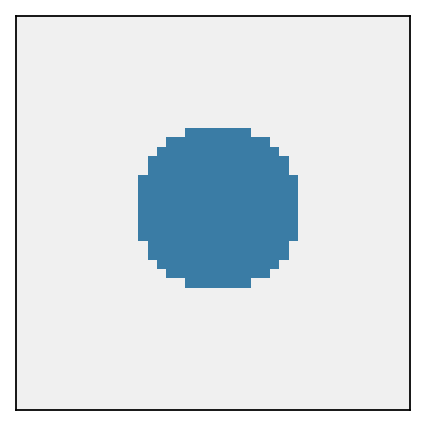
\includegraphics[width=0.22\textwidth]{transition_map_200ms.png} &
    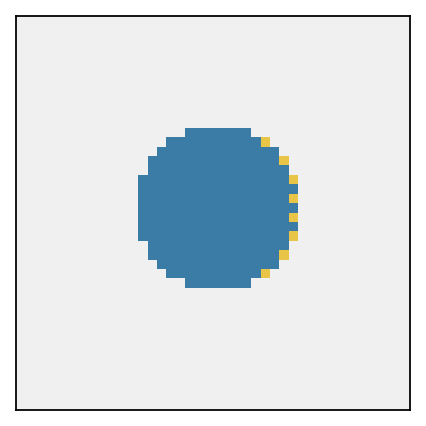
\includegraphics[width=0.22\textwidth]{transition_map_165ms.png} &
    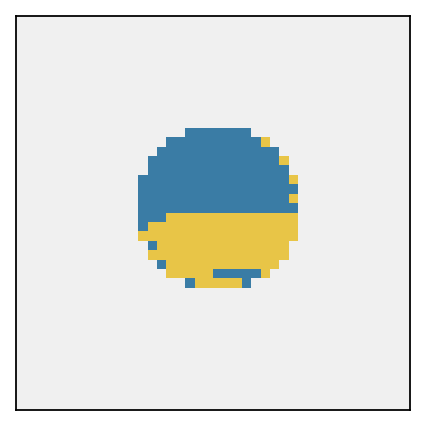
\includegraphics[width=0.22\textwidth]{transition_map_150ms.png} &
    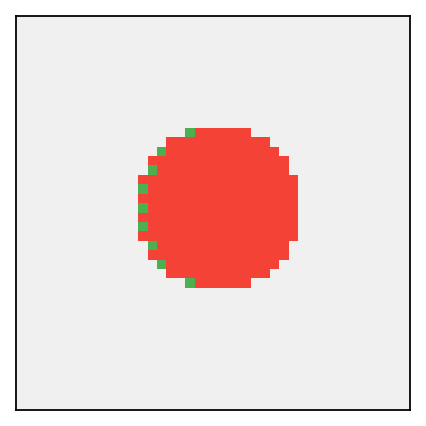
\includegraphics[width=0.22\textwidth]{transition_map_120ms.png} \\
    (a) 200\,ms & (b) 165\,ms & (c) 150\,ms & (d) 120\,ms \\
    \end{tabular}
    \caption{Wafer maps across the throughput--yield transition. At 165\,ms the first failures form an edge cluster at the row-change dies; the cluster persists through 150\,ms; by 120\,ms failure is near-total and the map saturates.}
    \label{fig:exp5_transition_maps}
\end{figure}

The results (Table~\ref{tab:exp5_transition}, Figure~\ref{fig:exp5_transition_maps}) confirm the mechanism precisely at the transition onset. At $t_{step} = 165$\,ms the first failures appear --- five dies with a row-change enrichment of \textbf{15.1}: every one of them is a die scanned immediately after a row change, clustering along one edge of the wafer, visually an \textit{Edge-Loc} morphology in the WM-811K taxonomy and produced purely by the motion profile. The onset is a plateau, not a knife edge: the cluster grows only to eight dies and holds at the same enrichment from 160 down to 150\,ms, and the wafer-wide collapse occurs between 150 and 120\,ms, where 232 of 241 dies fail and the map saturates into a \textit{Center}-classified blob. The wafer cycle time falls from 82.1 to 62.8\,s across the sweep, making the throughput--yield trade explicit: the settling budget between the clean 170\,ms wafer and the onset at 165\,ms buys nothing, while pushing from 150 to 120\,ms trades a 10\,\% cycle-time gain for almost the entire wafer.

Two observations qualify the classifier's part. The onset cluster is below the CNN's sensitivity --- it still reports \textit{none} at 97--98\,\%, and the cost even \textit{dips} at the onset (from 0.041 on the clean wafer to 0.027 at five failing dies): a reminder that the cost is a probability of morphology, not a die count, and the seed of the calibration behaviour Experiment 6 exposes. Only once the wafer saturates does the classifier leave \textit{none}, reading the 120\,ms map as \textit{Center} --- a class the corrected cost~\eqref{eq:cost_corrected} prices at its maximum as an out-of-domain signal rather than at zero. The informative segment of the cost curve --- exactly as anticipated --- is the transition region, and it is there that the optimizer of Experiment 6 operates.

\section{Experiment 6: Optimization Scenarios E3 and E4}\label{sec:exp_pso}

The final experiment runs the particle swarm of Section~\ref{sec:methodology_pso} twice over the same plant, controller (Case 3b), settling budget ($t_{step} = 150$\,ms, inside the transition region), and threshold, changing only the cost. Both scenarios carry a common throughput reward $\gamma\, T_{wafer}/T_{ref}$ ($\gamma = 1$, $T_{ref} = 15$\,s), so that a faster wafer is cheaper and the search actively trades cycle time against the map cost: scenario E3 pairs it with the conventional servo cost (wafer-average exposure MSD normalized by the threshold), scenario E4 with the yield-aware CNN cost~\eqref{eq:cost_corrected}. The question is what each cost is willing to trade throughput \textit{for}. The search runs over the exact fifteen-segment profile family, so all four bounds --- including $s_{\max}$ --- are live dimensions. Six particles run for eight iterations (48 full-wafer simulations per scenario), with one particle seeded at the baseline trajectory.

\begin{table}[htbp]
\centering
\caption{Optimization scenarios against the third- and fourth-order baselines at the same operating point ($t_{step} = 150$\,ms, Case 3b). Failing dies, CNN class, and $\mathcal{J}_{map}$ are evaluated on each trajectory's full-wafer map; $s$ is not a parameter of the third-order profile.}
\label{tab:exp6_pso}
\setlength{\tabcolsep}{0.12cm}
\begin{tabular}{lcccccccc}
\toprule
Scenario & $v$ [m/s] & $a$ [m/s$^2$] & $j$ [m/s$^3$] & $s$ [m/s$^4$] & Failing & CNN class & $\mathcal{J}_{map}$ & $T_{wafer}$ \\
\midrule
3rd-order baseline & 0.80 & 20.0 & 1600 & ---            & 44/49 & Center & 2.000 & 14.5\,s \\
4th-order baseline & 0.80 & 20.0 & 1600 & $10^5$         & 4/49  & none   & 0.038 & 15.2\,s \\
E3: servo cost     & 0.57 & 36.0 & 5000 & $1.5\times10^5$ & 4/49  & none   & 0.038 & 13.7\,s \\
E4: CNN cost       & 0.78 & 37.7 & 4840 & $3.4\times10^5$ & 5/49  & none   & 0.016 & 12.8\,s \\
\bottomrule
\end{tabular}
\end{table}

Both searches push the profile toward higher throughput, but they are stopped by different things (Table~\ref{tab:exp6_pso}). The servo cost is held back by error \textit{magnitude}: minimizing the wafer-average MSD keeps the velocity moderate ($v = 0.57$\,m/s) and the wafer at four failing dies, buying a 10\,\% shorter cycle than the fourth-order baseline (13.7 vs.\ 15.2\,s) without touching the yield. The CNN cost is held back only by pattern \textit{acceptability}: it drives the profile harder ($v = 0.78$\,m/s) and \textit{accepts a fifth failing die}, because the resulting scattered map still reads as a confident \textit{none} --- indeed $\mathcal{J}_{map}$ falls to 0.016, below the 0.038 of the four-die maps, since a few scattered failures are exactly what the classifier has learned a \textit{none} wafer looks like. That trade --- one more acceptable-pattern failure for a further 6\,\% of cycle time --- gives E4 the fastest wafer of the three (12.8\,s, 16\,\% below the baseline). The servo cost cannot make this trade: pricing error magnitude, it has no way to know that the extra failure is morphologically harmless.

Placed on the yield--throughput plane against the profile-order baselines, both optima dominate, and the two terms of the CNN cost are visibly doing distinct jobs. The regular fourth-order baseline (four dies, \textit{none}, 15.2\,s) is beaten on throughput by both; the third-order baseline collapses outright --- at the same tight settling budget its unbounded snap excites the chain so heavily that 44 of 49 dies fail and the map saturates to \textit{Center}, an out-of-domain morphology the cost prices at its maximum ($\mathcal{J}_{map} = 2.0$). This is exactly where the two halves of the CNN cost separate: the $(1-P_{none})$ term lets the optimizer spend an acceptable-pattern yield loss for throughput, while the $P_{ood}$ term is the wall that keeps it from cheapening the wafer into the \textit{Center} catastrophe of the third-order profile. The result confirms hypothesis H3 in the form it was posed --- the CNN-driven search converges to a profile that overcomes both the third-order and the regular fourth-order baselines on the yield--throughput plane --- with one honest qualification carried over from Experiment 3: on this bandwidth-limited plant the failing count is set mostly by the settling budget, so the yield the CNN cost trades away is modest (a single die), and a higher-bandwidth fine stage, where the profile controls more of the settling tail, would widen the margin the cost has to work with. The cost-evaluation history of both runs is archived with the experiment scripts.

\section{Experiment 7: Does Trajectory Smoothness Matter Without a Good Controller?}\label{sec:exp_order}

The premise of higher-order trajectory design is that bounding deeper derivatives injects less energy into the structure. A fair question is whether that refinement survives contact with a mediocre controller: if the tracking error is dominated by servo lag, does smoothing the reference accomplish anything at all? This experiment crosses the profile order --- acceleration-bounded (second order), jerk-bounded (third), and snap-bounded (fourth, exact fifteen-segment generator, plus a tight-snap variant at $s_{\max} = 2\times10^4$\,m/s$^4$) --- with the two ends of the controller ladder: bare collocated PID (Case 1) and feedforward plus fine-stage HIGS (Case 3b). All profiles run at the same kinematic bounds $(0.8, 20, 1600)$ on the four-die row.

\begin{table}[htbp]
\centering
\caption{Profile order $\times$ controller. Cruise indices of $e_{syn}$ (worst die); full-scan MSD includes the post-step entry transient.}
\label{tab:exp7_order}
\setlength{\tabcolsep}{0.14cm}
\begin{tabular}{llcccc}
\toprule
Profile & Controller & $T_{scan}$ & cruise max$|$MA$|$ & cruise max MSD & full-scan MSD \\
\midrule
2nd order & Case 1  & 132.5\,ms & 668\,\textmu m & 43.2\,\textmu m & 232\,\textmu m \\
3rd order & Case 1  & 145.0\,ms & 770\,\textmu m & 27.2\,\textmu m & 155\,\textmu m \\
4th order & Case 1  & 160.8\,ms & 817\,\textmu m & 19.7\,\textmu m & 87.7\,\textmu m \\
4th, tight snap & Case 1 & 208.6\,ms & 616\,\textmu m & 9.93\,\textmu m & 55.4\,\textmu m \\
\midrule
2nd order & Case 3b & 132.5\,ms & 3.56\,\textmu m & 0.968\,\textmu m & 2.56\,\textmu m \\
3rd order & Case 3b & 145.0\,ms & 1.85\,\textmu m & 0.266\,\textmu m & 0.51\,\textmu m \\
4th order & Case 3b & 160.8\,ms & 0.873\,\textmu m & 0.096\,\textmu m & 0.34\,\textmu m \\
4th, tight snap & Case 3b & 208.6\,ms & \textbf{0.201}\,\textmu m & \textbf{0.0185}\,\textmu m & 0.34\,\textmu m \\
\bottomrule
\end{tabular}
\end{table}

\begin{figure}[htbp]
    \centering
    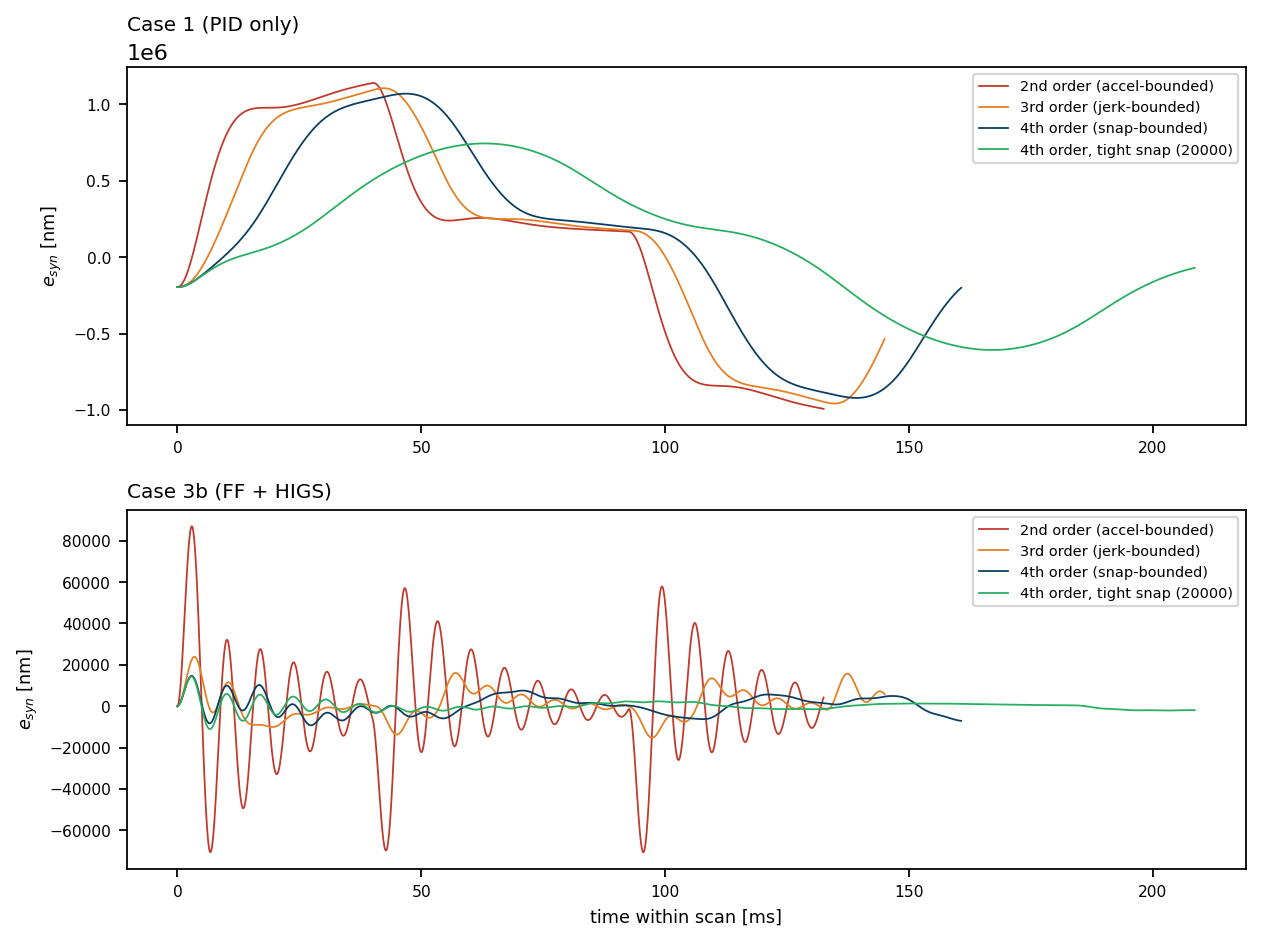
\includegraphics[width=0.9\textwidth]{order_comparison_esyn.png}
    \caption{Synchronization error during one scan for the four profile orders, under bare PID (top) and under the full controller ladder (bottom). Note the vertical scales.}
    \label{fig:exp7_order}
\end{figure}

The answer is layered (Table~\ref{tab:exp7_order}, Figure~\ref{fig:exp7_order}). \textbf{Under the bare PID, trajectory order reaches the exposure only through the transients.} The cruise MA sits at 0.6--0.8\,mm for every order --- it is the slowly decaying tail of the acceleration transient, which the collocated loop cannot reject, and reference smoothness does not remove it within the cruise window. Order does shape how much transient there is to decay: the cruise MSD improves monotonically with smoothness, $43.2 \rightarrow 27.2 \rightarrow 19.7 \rightarrow 9.93$\,\textmu m from second order to tight snap ($4.4\times$), and the full-scan MSD follows the same ordering ($232 \rightarrow 55$\,\textmu m); the reduction is real but the exposure error remains dominated by what the controller leaves behind.

\textbf{Under the full ladder, trajectory order is worth an order of magnitude.} With the feedforward removing the quasi-static lag and the HIGS loop suppressing what lies within its bandwidth, the cruise MSD falls $0.97 \rightarrow 0.27 \rightarrow 0.096$\,\textmu m from second to fourth order --- a $10\times$ improvement attributable to the profile alone, at identical kinematic bounds, and $52\times$ to the tight-snap variant (18.5\,nm). The interpretation is classical and now quantified for this plant: the fine loop handles the error components inside its bandwidth, and the profile order determines how much excitation exists \textit{beyond} it; smoothing the reference and improving the controller are complements, not substitutes. Two further readings matter for the optimizer. First, smoothness has a throughput price --- $T_{scan}$ grows 21\,\% from second to fourth order at the same bounds, and a further 30\,\% for the tight-snap variant --- so profile order participates in the same throughput--yield trade as the kinematic bounds themselves. Second, the tight-snap variant is the \textit{most} accurate configuration in the cruise (MSD 18.5\,nm, MA 0.20\,\textmu m --- the closest any configuration of this plant comes to the nanometre specifications), yet its full-scan MSD is no better than the plain fourth-order profile's (0.34\,\textmu m for both, set by the post-step entry transient) while it spends 30\,\% more scan time. Accuracy inside the cruise keeps improving with smoothness, while the settling-dominated component saturates at the closed loop's floor and the throughput cost grows without bound: the optimum in the snap dimension is therefore interior once throughput enters the cost --- precisely the trade the optimizer of Experiment 6 is built to resolve.

\section{A Recurrent Surrogate Model (Secondary Study)}\label{sec:exp_surrogate}

This closing study is deliberately \textit{secondary}: the main line of the thesis --- trajectory generation, control, defect mapping, CNN cost, and optimization --- does not depend on it, and Experiment 6 runs its optimization against the full simulation directly. The recurrent surrogate of Section~\ref{sec:methodology_surrogate}, trained on 100 randomized simulation runs ($\approx 1.6$ million samples), is evaluated in two roles: as a fast predictor of the exposure indices for individual candidate trajectories, and as the inner evaluation of a grid search over the kinematic bounds.

Table~\ref{tab:exp4_lstm} shows the surrogate's predictions for three trajectories of decreasing aggressiveness, after retraining on the corrected plant. The predicted indices decrease monotonically --- by a factor of 30 on MA and 45 on MSD between the baseline and the slowest candidate --- reproducing the ordering observed in the full simulation. Their absolute scale, however, inherits the constant geometric offset present in the synchronization-error signal on which the surrogate was trained, so the predictions are meaningful for \textit{ranking} candidates rather than for verifying absolute compliance; all three candidates are correctly rejected against the nanometre thresholds.

\begin{table}[htbp]
\centering
\caption{Surrogate predictions of the exposure indices for three candidate trajectories.}
\label{tab:exp4_lstm}
\begin{tabular}{ccccccc}
\toprule
$v_{\max}$ [m/s] & $a_{\max}$ [m/s$^2$] & $j_{\max}$ [m/s$^3$] & $s_{\max}$ [m/s$^4$] & $\max|\mathrm{MA}|$ & $\max \mathrm{MSD}$ & Verdict \\
\midrule
0.80 & 20.0 & 1600 & $10^5$ & 31.5\,mm  & 5.26\,mm  & FAIL \\
0.10 & 1.0  & 100  & $10^4$ & 2.28\,mm  & 0.46\,mm  & FAIL \\
0.01 & 0.1  & 1    & 10     & 1.09\,mm  & 0.118\,mm & FAIL \\
\bottomrule
\end{tabular}
\end{table}

The grid search evaluates 450 configurations over $v \in [0.01, 0.5]$\,m/s, $a \in [0.1, 10]$\,m/s$^2$, $j \in \{500, 1000, 2000\}$\,m/s$^3$, $s \in \{10^4, 5\times10^4, 10^5\}$\,m/s$^4$, accepting a candidate only if the predicted indices satisfy the nanometre specifications. The search terminates without finding any feasible candidate and reports that the sub-nanometre regime is unreachable for the Case 1 machine, recommending the spring-compensation or fine-stage configurations of the reference study. This negative result is consistent with Experiment 1 and with the sweep of Experiment 3: in a coarse-only machine, no admissible trajectory can suppress the reticle-coupling error to nanometre level, since the dominant error term is structural rather than kinematic.

\subsection{Is a recurrent surrogate the right tool?}\label{sec:exp_surrogate_critique}

The results above prompt a question that the thesis should answer explicitly rather than assume: does a learned sequence model make sense for this plant at all?

For the Case 1 configuration as simulated, the honest answer is that it is not \textit{necessary}. The plant is linear time-invariant --- linear Kelvin--Voigt couplings, linear PID feedback, linear feedforward --- so the map from the reference kinematics to the synchronization error is an exact, known LTI operator. It can be evaluated by directly integrating the reduced two-body model (seconds per candidate, Experiment 1) or captured without error by a fitted low-order transfer function, with no training data and full interpretability. A GRU trained on one hundred randomized runs approximates something that, in this regime, can be computed exactly; its only measured advantage is evaluation speed against the \textit{full} MuJoCo model, not against the reduced model that suffices for Case 1. The training data also transferred a defect into the surrogate: the synchronization-error signal it learned from contains the constant geometric offset of the absolute coordinates, which is why the predictions of Table~\ref{tab:exp4_lstm} rank correctly but carry a meaningless absolute scale.

The recurrent surrogate earns its place under three conditions that define the continuation of this work, none of which holds in the linear baseline but all of which appear in the target configurations. First, \textit{nonlinearity}: the actuator saturation ($5\times10^4$\,N) engaged by aggressive transients, and above all the nonlinear feedback structures planned for the fine-stage configurations (reset elements and hybrid integrator--gain systems~\cite{Heertjes2025_NonlinearControl}), break the LTI shortcut --- there is then no exact transfer function to fit, and a learned dynamic model becomes a legitimate system-identification tool. Second, \textit{cost amortization}: when the evaluation plant is the full multi-body simulation over a complete 241-die wafer (minutes per candidate, Experiment 3) inside a population-based optimizer issuing thousands of evaluations, a millisecond surrogate changes what is computationally feasible. Third, \textit{inter-segment memory}: the recurrent state carries transients across the scan--step--scan sequence, an effect that static regressions over $(v_{\max}, a_{\max}, j_{\max}, s_{\max})$ cannot represent and that grows in importance as settling budgets shrink.

Three concrete amendments follow for the next iteration of the surrogate: retrain on the offset-corrected error signal, so that absolute predictions become meaningful against the MA/MSD thresholds; report ranking fidelity (for example rank correlation against full-simulation sweeps) as the primary metric, since ranking is what the optimizer consumes; and benchmark against the LTI baseline on Case 1, so that the surrogate's added value is demonstrated where it exists --- the nonlinear, full-model configurations --- rather than presumed everywhere.

\section{Discussion}\label{sec:exp_discussion}

Read against the evaluation scenarios of the thesis proposal --- E1: third-order baseline, E2: fourth-order baseline, E3: optimization under a servo cost, E4: optimization under the CNN cost --- the experiments above address all four: the trajectory generator, the validated plant, the controller ladder up to the nonlinear HIGS loop, the trained classifier, the trajectory-to-map bridge, and two full optimization runs differing only in their cost. The third-versus-fourth-order comparison of E1 and E2 is delivered directly by the order study of Experiment 7, now that the exact segment generators represent every profile order by its true shape rather than by a polynomial approximation.

Of the validation criterion, three elements are now satisfied: unperturbed operation maps to the \textit{none} class; the cost input shifts monotonically and reproducibly under parameter sweeps; and --- the strongest result of the campaign --- spatially structured, scanner-plausible morphology emerges from the motion profile itself, with the transition onset of Experiment 5 concentrating its first failures at the row-change dies with fifteen-fold enrichment, an \textit{Edge-Loc} pattern requiring no injected disturbance.

The class-level half of the criterion --- that motion-induced failures be \textit{classified} into the scanner-plausible classes --- is met only partially, and every failure mode observed points at the classifier rather than at the simulation half of the pipeline. The scratch-shaped disturbance cannot be recognized as \textit{Scratch} while the classifier's recall for that class is zero (Experiment 2), so the 15-die column falls to \textit{Loc}; dense scattered patterns are absorbed into \textit{Center}; the drift annulus is read as \textit{Donut}; the Edge-Loc onset of Experiment 5 sits below the classifier's sensitivity; and the classifier prices \textit{morphology}, not die count, so on the near-clean plateau it reads every sparse-failure wafer as \textit{none}. Experiment 6 turned that last property to advantage --- it is exactly what lets the yield-aware cost trade an acceptable-pattern failure for throughput --- but it also means the cost cannot, on its own, resolve fine yield differences the classifier was never trained to see. The refinement list is correspondingly concrete and bounded: rebalanced training for the minority classes (above all \textit{Scratch}) and probability calibration on clean and near-clean maps, so that motion-induced scratch and edge morphologies are recognized as themselves rather than as their nearest well-populated neighbour. On the trajectory side the exact generators are now in place, and Experiment 7 showed that profile order is worth an order of magnitude of exposure error under a capable controller, with the snap trade-off resolved by throughput rather than by accuracy alone. On the plant side, the corrections carried through this iteration --- error-velocity servo damping on the frictionless guideways, balance-mass cancellation of the actuator reactions, and consistently paired error sampling --- hold the exposure error at the sub-micrometre scale under the full ladder; the remaining order of magnitude to the reference machine's tens-of-nanometre two-stage result belongs to servo bandwidth, the generic $100$\,rad/s fine loop modelled here against the reference's high-bandwidth positioning subsystem. None of these items changes the architecture validated here: generate, track, map, classify, price, and optimize --- the loop is closed and runs end to end.

%%% ----------------------------------------------------------------------


\def\baselinestretch{1}
\nonumchapter{Conclusion}\label{ch:conclusion}
\def\baselinestretch{1.1}

En este trabajo de investigacion se ha propuesto un esquema de ...

\goodbreak
%%% ----------------------------------------------------------------------
 %adds conclusions
% ------------------------------------------------------------------------
% BIBLIOGRAPHY:
\setlinespacing{0.70} %spacing
\bibliographystyle{amsplain} %bibliography style
%\setcounter{page}{xx} %restarts counter at page xx
\bibliography{bibliografia} %directly in the folder
%\bibliography{C:/Users/User1/Desktop/tesis/Latexf\string~1/folderbib/bibliografia} %path of a special folder
% ------------------------------------------------------------------------
% Appendices:
\setlinespacing{0.60} %spacing
\appendix %adds appendices
\def\baselinestretch{1}
\chapter{Full-State Space Model}
\def\baselinestretch{1.1}

\section{State-Space Equations for the Wafer Chain}\label{ape:waferchainequations}

The wafer chain corresponds to $j=3$, with $N_3=7$ (bodies $i=2, \ldots, 7$). These map to global state vectors $\mathbf{x}_{2p-1}$ (translational) and $\mathbf{x}_{2p}$ (rotational) for $p=12, \ldots, 17$. The state-space equations are represented below.

\textbf{First body of the wafer chain ($i=2$, $p=12$):}
\begin{align}
    \ddot{\mathbf{x}}_{23} &= 
    \frac{1}{\bar{m}_{2_3}} \Big[ u^0_{2_3} - {}^0\bar{C}_{2_3}\dot{\mathbf{x}}_{23} - {}^0\bar{K}_{2_3}\mathbf{x}_{23} + {}^0\hat{C}_{3_3}\dot{\mathbf{x}}_{25} + {}^0\hat{K}_{3_3}\mathbf{x}_{25} \Big] \notag \\
    &\quad - \frac{1}{m_0} \Big[ u^0_1 - {}^0\bar{C}_1\dot{\mathbf{x}}_{1} - {}^0\bar{K}_1 \mathbf{x}_{1} + \sum_{k=1}^3 \left( {}^0\hat{C}_{2_k}\dot{\mathbf{x}}_{2p_{2_k}-1} + {}^0\hat{K}_{2_k}\mathbf{x}_{2p_{2_k}-1} \right) \Big] \\
    \ddot{\mathbf{x}}_{24} &= 
    \frac{1}{I_{z_{2_3}}} \Big[ \tau^0_{2_3} - {}^0\bar{c}_{\theta,2_3}\dot{\mathbf{x}}_{24} - {}^0\bar{k}_{\theta,2_3}\mathbf{x}_{24} + {}^0\hat{c}_{\theta,3_3}\dot{\mathbf{x}}_{26} + {}^0\hat{k}_{\theta,3_3}\mathbf{x}_{26} \Big] \notag \\
    &\quad - \frac{1}{I_{z_0}} \Big[ \tau^0_1 - {}^0\bar{C}_1\dot{\mathbf{x}}_{2} - {}^0\bar{K}_1 \mathbf{x}_{2} + \sum_{k=1}^3 \left( {}^0\hat{c}_{\theta,2_k}\dot{\mathbf{x}}_{2p_{2_k}} + {}^0\hat{k}_{\theta,2_k}\mathbf{x}_{2p_{2_k}} \right) \Big]
\end{align}

\textbf{Intermediate body ($i=3$, $p=13$):}
\begin{align}
    \ddot{\mathbf{x}}_{25} &= 
    \frac{1}{\bar{m}_{3_3}} \Big[ u^0_{3_3} - {}^0\bar{C}_{3_3}\dot{\mathbf{x}}_{25} - {}^0\bar{K}_{3_3}\mathbf{x}_{25} + {}^0\hat{C}_{(4)_3}\dot{\mathbf{x}}_{27} + {}^0\hat{K}_{(4)_3}\mathbf{x}_{27} \Big] \notag \\
    &\quad - \frac{1}{\bar{m}_{(2)_3}} \Big[ u^0_{(2)_3} - {}^0\bar{C}_{(2)_3}\dot{\mathbf{x}}_{23} - {}^0\bar{K}_{(2)_3}\mathbf{x}_{23} + {}^0\hat{C}_{3_3}\dot{\mathbf{x}}_{25} + {}^0\hat{K}_{3_3}\mathbf{x}_{25} \Big] \\
    \ddot{\mathbf{x}}_{26} &= 
    \frac{1}{I_{z_{3_3}}} \Big[ \tau^0_{3_3} - {}^0\bar{c}_{\theta,3_3}\dot{\mathbf{x}}_{26} - {}^0\bar{k}_{\theta,3_3}\mathbf{x}_{26} + {}^0\hat{c}_{\theta,(4)_3}\dot{\mathbf{x}}_{28} + {}^0\hat{k}_{\theta,(4)_3}\mathbf{x}_{28} \Big] \notag \\
    &\quad - \frac{1}{I_{z_{(2)_3}}} \Big[ \tau^0_{(2)_3} - {}^0\bar{c}_{\theta,(2)_3}\dot{\mathbf{x}}_{24} - {}^0\bar{k}_{\theta,(2)_3}\mathbf{x}_{24} + {}^0\hat{c}_{\theta,3_3}\dot{\mathbf{x}}_{26} + {}^0\hat{k}_{\theta,3_3}\mathbf{x}_{26} \Big]
\end{align}

\textbf{Intermediate body ($i=4$, $p=14$):}
\begin{align}
    \ddot{\mathbf{x}}_{27} &= 
    \frac{1}{\bar{m}_{4_3}} \Big[ u^0_{4_3} - {}^0\bar{C}_{4_3}\dot{\mathbf{x}}_{27} - {}^0\bar{K}_{4_3}\mathbf{x}_{27} + {}^0\hat{C}_{(5)_3}\dot{\mathbf{x}}_{29} + {}^0\hat{K}_{(5)_3}\mathbf{x}_{29} \Big] \notag \\
    &\quad - \frac{1}{\bar{m}_{(3)_3}} \Big[ u^0_{(3)_3} - {}^0\bar{C}_{(3)_3}\dot{\mathbf{x}}_{25} - {}^0\bar{K}_{(3)_3}\mathbf{x}_{25} + {}^0\hat{C}_{4_3}\dot{\mathbf{x}}_{27} + {}^0\hat{K}_{4_3}\mathbf{x}_{27} \Big] \\
    \ddot{\mathbf{x}}_{28} &= 
    \frac{1}{I_{z_{4_3}}} \Big[ \tau^0_{4_3} - {}^0\bar{c}_{\theta,4_3}\dot{\mathbf{x}}_{28} - {}^0\bar{k}_{\theta,4_3}\mathbf{x}_{28} + {}^0\hat{c}_{\theta,(5)_3}\dot{\mathbf{x}}_{30} + {}^0\hat{k}_{\theta,(5)_3}\mathbf{x}_{30} \Big] \notag \\
    &\quad - \frac{1}{I_{z_{(3)_3}}} \Big[ \tau^0_{(3)_3} - {}^0\bar{c}_{\theta,(3)_3}\dot{\mathbf{x}}_{26} - {}^0\bar{k}_{\theta,(3)_3}\mathbf{x}_{26} + {}^0\hat{c}_{\theta,4_3}\dot{\mathbf{x}}_{28} + {}^0\hat{k}_{\theta,4_3}\mathbf{x}_{28} \Big]
\end{align}

\textbf{Intermediate body ($i=5$, $p=15$):}
\begin{align}
    \ddot{\mathbf{x}}_{29} &= 
    \frac{1}{\bar{m}_{5_3}} \Big[ u^0_{5_3} - {}^0\bar{C}_{5_3}\dot{\mathbf{x}}_{29} - {}^0\bar{K}_{5_3}\mathbf{x}_{29} + {}^0\hat{C}_{(6)_3}\dot{\mathbf{x}}_{31} + {}^0\hat{K}_{(6)_3}\mathbf{x}_{31} \Big] \notag \\
    &\quad - \frac{1}{\bar{m}_{(4)_3}} \Big[ u^0_{(4)_3} - {}^0\bar{C}_{(4)_3}\dot{\mathbf{x}}_{27} - {}^0\bar{K}_{(4)_3}\mathbf{x}_{27} + {}^0\hat{C}_{5_3}\dot{\mathbf{x}}_{29} + {}^0\hat{K}_{5_3}\mathbf{x}_{29} \Big] \\
    \ddot{\mathbf{x}}_{30} &= 
    \frac{1}{I_{z_{5_3}}} \Big[ \tau^0_{5_3} - {}^0\bar{c}_{\theta,5_3}\dot{\mathbf{x}}_{30} - {}^0\bar{k}_{\theta,5_3}\mathbf{x}_{30} + {}^0\hat{c}_{\theta,(6)_3}\dot{\mathbf{x}}_{32} + {}^0\hat{k}_{\theta,(6)_3}\mathbf{x}_{32} \Big] \notag \\
    &\quad - \frac{1}{I_{z_{(4)_3}}} \Big[ \tau^0_{(4)_3} - {}^0\bar{c}_{\theta,(4)_3}\dot{\mathbf{x}}_{28} - {}^0\bar{k}_{\theta,(4)_3}\mathbf{x}_{28} + {}^0\hat{c}_{\theta,5_3}\dot{\mathbf{x}}_{30} + {}^0\hat{k}_{\theta,5_3}\mathbf{x}_{30} \Big]
\end{align}

\textbf{Intermediate body ($i=6$, $p=16$):}
\begin{align}
    \ddot{\mathbf{x}}_{31} &= 
    \frac{1}{\bar{m}_{6_3}} \Big[ u^0_{6_3} - {}^0\bar{C}_{6_3}\dot{\mathbf{x}}_{31} - {}^0\bar{K}_{6_3}\mathbf{x}_{31} + {}^0\hat{C}_{(7)_3}\dot{\mathbf{x}}_{33} + {}^0\hat{K}_{(7)_3}\mathbf{x}_{33} \Big] \notag \\
    &\quad - \frac{1}{\bar{m}_{(5)_3}} \Big[ u^0_{(5)_3} - {}^0\bar{C}_{(5)_3}\dot{\mathbf{x}}_{29} - {}^0\bar{K}_{(5)_3}\mathbf{x}_{29} + {}^0\hat{C}_{6_3}\dot{\mathbf{x}}_{31} + {}^0\hat{K}_{6_3}\mathbf{x}_{31} \Big] \\
    \ddot{\mathbf{x}}_{32} &= 
    \frac{1}{I_{z_{6_3}}} \Big[ \tau^0_{6_3} - {}^0\bar{c}_{\theta,6_3}\dot{\mathbf{x}}_{32} - {}^0\bar{k}_{\theta,6_3}\mathbf{x}_{32} + {}^0\hat{c}_{\theta,(7)_3}\dot{\mathbf{x}}_{34} + {}^0\hat{k}_{\theta,(7)_3}\mathbf{x}_{34} \Big] \notag \\
    &\quad - \frac{1}{I_{z_{(5)_3}}} \Big[ \tau^0_{(5)_3} - {}^0\bar{c}_{\theta,(5)_3}\dot{\mathbf{x}}_{30} - {}^0\bar{k}_{\theta,(5)_3}\mathbf{x}_{30} + {}^0\hat{c}_{\theta,6_3}\dot{\mathbf{x}}_{32} + {}^0\hat{k}_{\theta,6_3}\mathbf{x}_{32} \Big]
\end{align}

\textbf{End-effector body ($i=7$, $p=17$):}
\begin{align}
    \ddot{\mathbf{x}}_{33} &= 
    \frac{1}{\bar{m}_{7_3}} \Big[ u^0_{7_3} - {}^0\bar{C}_{7_3}\dot{\mathbf{x}}_{33} - {}^0\bar{K}_{7_3}\mathbf{x}_{33} \Big] \notag \\
    &\quad - \frac{1}{\bar{m}_{(6)_3}} \Big[ u^0_{(6)_3} - {}^0\bar{C}_{(6)_3}\dot{\mathbf{x}}_{31} - {}^0\bar{K}_{(6)_3}\mathbf{x}_{31} + {}^0\hat{C}_{7_3}\dot{\mathbf{x}}_{33} + {}^0\hat{K}_{7_3}\mathbf{x}_{33} \Big] \\
    \ddot{\mathbf{x}}_{34} &= 
    \frac{1}{I_{z_{7_3}}} \Big[ \tau^0_{7_3} - {}^0\bar{c}_{\theta,7_3}\dot{\mathbf{x}}_{34} - {}^0\bar{k}_{\theta,7_3}\mathbf{x}_{34} \Big] \notag \\
    &\quad - \frac{1}{I_{z_{(6)_3}}} \Big[ \tau^0_{(6)_3} - {}^0\bar{c}_{\theta,(6)_3}\dot{\mathbf{x}}_{32} - {}^0\bar{k}_{\theta,(6)_3}\mathbf{x}_{32} + {}^0\hat{c}_{\theta,7_3}\dot{\mathbf{x}}_{34} + {}^0\hat{k}_{\theta,7_3}\mathbf{x}_{34} \Big]
\end{align}

%%%%%%%%%%%%%%%%%%%%%%%%%%%%%%%%%%%%%%%%%%%%%%%%%%%%%%%%%%%%%%%%%%%%%%%%%%%%%%%%%%%%%%% %chapter appendix1
% ------------------------------------------------------------------------
\end{document}
